\documentclass[semifinal]{cpecmu}

%% This is a sample document demonstrating how to use the CPECMU
%% project template. If you are having trouble, see "cpecmu.pdf" for
%% documentation.

\projectNo{P003-2}
\acadyear{2022}

\titleTH{เว็บแอพพลิเคชันสำหรับจับคู่เพื่อนร่วมห้องและจองหอพักในมหาวิทยาลัย}
\titleEN{Web application for matching roommates and booking campus dormitory}

\author{นายกมลพัฒน์ สุนทรพงศ์}{Kamonpat Sunthonpong}{620610771}

\cpeadvisor{chinawat}
\cpecommittee{navadon}
\cpecommittee{juggapong}

%% Some possible packages to include:
\usepackage[final]{graphicx} % for including graphics

%% Add bookmarks and hyperlinks in the document.
\PassOptionsToPackage{hyphens}{url}
\usepackage[colorlinks=true,allcolors=Blue4,citecolor=red,linktoc=all]{hyperref}
\def\UrlFont{\thaifonttt}

%% Set up commenting
\iffinal
  \usepackage[disabled]{authcomments}
\else
  \usepackage{authcomments}
\fi
\newcommenter{CI}{0.0,0.5625,0.0}  % green

\newcommenter{ME}{1.0,0,0} % my red comment 

%% Needed just by this example, but maybe not by most reports
\usepackage{afterpage} % for outputting
\usepackage{pdflscape} % for landscape figures and tables. 

%% Some other useful packages. Look these up to find out how to use
%% them.
% \usepackage{natbib}    % for author-year citation styles
% \usepackage{txfonts}
% \usepackage{appendix}  % for appendices on a per-chapter basis
% \usepackage{xtab}      % for tables that go over multiple pages
% \usepackage{subfigure} % for subfigures within a figure
% \usepackage{pstricks,pdftricks} % for access to special PostScript and PDF commands
% \usepackage{nomencl}   % if you have a list of abbreviations

%% if you're having problems with overfull boxes, you may need to increase
%% the tolerance to 9999
% \tolerance=9999

\bibliographystyle{plain}
% \bibliographystyle{IEEEbib}
% \renewcommand{\topfraction}{0.85}
% \renewcommand{\textfraction}{0.1}
% \renewcommand{\floatpagefraction}{0.75}

%% Example for glossary entry
%% Need to use glossary option
%% See glossaries package for complete documentation.
\ifglossary
  \newglossaryentry{lorem ipsum}{
    name=lorem ipsum,
    description={derived from Latin dolorem ipsum, translated as ``pain itself''}
  }
\fi

%% Uncomment this command to preview only specified LaTeX file(s)
%% imported with \include command below.
%% Any other file imported via \include but not specified here will not
%% be previewed.
%% Useful if your report is large, as you might not want to build
%% the entire file when editing a certain part of your report.
% \includeonly{chapters/intro,chapters/background}

\begin{document}
\maketitle
\makesignature

\ifproject
  \begin{abstractTH}
    
    ในปัจจุบันระบบจองหอพักในของนักศึกษามหาวิทยาลัยเชียงใหม่ กำลังประสบปัญหานักศึกษาไม่ได้พัก
    อาศัยกับเพื่อนร่วมห้อง หรือห้องพักที่ต้องการ อันเนื่องมาจากการแข่งขันในช่วงเวลาประมวลผลของระบบ
    เพื่อแก้ไขปัญหาดังกล่าว โครงงานนี้จึงได้เสนอแอพพลิเคชันใหม่ ที่อนุญาตให้ผู้ใช้ระบุห้อง 
    และเพื่อนร่วมห้องตามความต้องการ หลังจากนั้นระบบจะทำการจับคู่ให้แบบอัตโนมัติ 
    โดยอิงจากความคล้ายคลึงกันของความต้องการของแต่ละฝ่าย ด้วยวิธีนี้แอพพลิเคชันใหม่นี้มุ่งเน้นที่จะพัฒนา 
    ให้ผู้ใช้ได้รับประสบการณ์การจองหอพักที่มีประสิทธิภาพยิ่งขึ้น
    
    % การเขียนรายงานเป็นส่วนหนึ่งของการทำโครงงานวิศวกรรมคอมพิวเตอร์
    % เพื่อทบทวนทฤษฎีที่เกี่ยวข้อง อธิบายขั้นตอนวิธีแก้ปัญหาเชิงวิศวกรรม และวิเคราะห์และสรุปผลการทดลองอุปกรณ์และระบบต่างๆ
    % \enskip อย่างไรก็ดี การสร้างรูปเล่มรายงานให้ถูกรูปแบบนั้นเป็นขั้นตอนที่ยุ่งยาก
    % แม้ว่าจะมีต้นแบบสำหรับใช้ในโปรแกรม Microsoft Word แล้วก็ตาม
    % แต่นักศึกษาส่วนใหญ่ยังคงค้นพบว่าการใช้งานมีความซับซ้อน และเกิดความผิดพลาดในการจัดรูปแบบ กำหนดเลขหัวข้อ และสร้างสารบัญอยู่
    % \enskip ภาควิชาวิศวกรรมคอมพิวเตอร์จึงได้จัดทำต้นแบบรูปเล่มรายงานโดยใช้ระบบจัดเตรียมเอกสาร
    % \LaTeX{} เพื่อช่วยให้นักศึกษาเขียนรายงานได้อย่างสะดวกและรวดเร็วมากยิ่งขึ้น
  \end{abstractTH}
  
  \begin{abstract}
    
   Chiang Mai University dormitory booking system is facing the problem of 
   students being unable to secure their preferred rooms or roommates due to
   the competition in processing period. To address this issue, this project 
   proposes a new web application that will allow users to specify their roommate
   and rooms preferences. The application will then automatically match users based
   on the similarity of their preferences, improving the chances of students getting
   their preferred accommodations. In this way, the new application aims to provide
   a more efficient booking experience for students of Chiang Mai University.
    
    % The abstract would be placed here. It usually does not exceed 350 words
    % long (not counting the heading), and must not take up more than one (1) page
    % (even if fewer than 350 words long).
    
    % Make sure your abstract sits inside the \texttt{abstract} environment.
  \end{abstract}
  
  \iffalse
    \begin{dedication}
      This document is dedicated to all Chiang Mai University students.
      
      Dedication page is optional.
    \end{dedication}
  \fi % \iffalse
  
  \begin{acknowledgments}
    โครงการนี้จะไม่สามารถสำเร็จได้ ถ้าไม่ได้รับความกรุณาจาก อ.ดร. ชินวัตร อิศราดิสัยกุล 
    อาจารย์ที่ปรึกษาโครงการที่คอยให้ความช่วยเหลือ เสนอแนะแนวทางในการแก้ปัญหา 
    คอยติดตามงาน และจัดลำดับความสำคัญงานอยู่เสมอ

    ขอขอบคุณภาควิชาวิศวกรรมคอมพิวเตอร์ คณะวิศวกรรมศาสตร์ มหาวิทยาลัยเชียงใหม่ 
    ที่มอบทุนสนับสนุนการพัฒนา และเอื้อเฟื้อสถานที่ในการจัดทำโครงการนี้

    ขอขอบคุณสำนักงานพัฒนาวิทยาศาสตร์และเทคโนโลยีแห่งชาติ สถาบันเทคโนโลยี
    อิเล็กทรอนิกส์และคอมพิวเตอร์แห่งชาติ ที่มอบทุนสนับสนุนการพัฒนาโครงการนี้ 
    ผ่านโครงการแข่งขันพัฒนาโปรแกรมคอมพิวเตอร์แต่งประเทศไทยครั้้งที่ 25
    % Your acknowledgments go here. Make sure it sits inside the
    % \texttt{acknowledgment} environment.
    
    \acksign{2023}{3}{20}
  \end{acknowledgments}%
\fi % \ifproject

\contentspage

\ifproject
  \figurelistpage
  
  \tablelistpage
\fi % \ifproject

% \abbrlist % this page is optional

% \symlist % this page is optional

% \preface % this section is optional


\pagestyle{empty} \cleardoublepage
\normalspacing \setcounter{page}{1} \pagenumbering{arabic} \pagestyle{cpecmu}

\chapter{\ifenglish Introduction \else บทนำ\fi}
\section{\ifenglish Project rationale\else ที่มาของโครงงาน\fi}

\MEreply{use โครงการ not  โครงงาน}
\MEreply{
    \begin{itemize}
        \item describe current system, user flow ans result
        \item how system cause the issues user acceptance
        \item -----------"--------------- traffic then load then low avaiability make even worse
        \item how to solve this problem
    \end{itemize}
}
\ME{
    ในการจองหอพักของมหาวิทยาลัยเชียงใหม่นั้น มีขั้นตอนการทำงานดังต่อไปนี้
    \begin{enumerate}
        \item นักศึกษาลงชื่อเข้าใช้งานระบบ
        \item นักศึกษาเลือกหอพักที่ต้องการจอง
        \item นักศึกษาเลือกห้องพักที่ต้องการพักอาศัย
        \item กดยืนยันการจองห้องพัก
    \end{enumerate}
    ซึ่งเป็นระบบที่เรียบง่าย และไม่มีความซับซ้อน แต่ทว่าเพื่อให้สอดคล้องกับระบบการรับนักศึกษา TCAS 
    ที่แบ่งรอบการรับนักศึกษาเป็นหลายๆ รอบ ทำให้ผู้ดูแลหอพักต้องแบ่งสำรองจำนวนห้องพักที่สามารถจองได้ในแต่ละรอบ
    ทำให้ในแต่ละรอบนั้นจะมีห้องว่างที่ไม่สามารถเปิดให้ นักศึกษาที่สอบผ่านเป็นรอบแรกๆ ได้จองห้องเหล่านั้น 
    จึงกลายเป็นปัญหาขึ้นในระบบการจองหอพัก
}
{first item of guideline}

ระบบจองหอพักนักศึกษามหาวิทยาลัยเชียงใหม่ประสบปัญหาหลายประการ ที่อาจทำให้นักศึกษายากที่จะจองหอพัก 
และหาห้องพักที่เหมาะสม ปัญหาหนึ่งคือความไม่เพียงพอของข้อมูลเกี่ยวกับผู้เข้าพักร่วม 
เนื่องจากในขั้นตอนการจองห้องนั้นนักศึกษาจะมองเห็นเพียงชื่อของนักศึกษาที่จองห้องพักเดียวกัน
นักศึกษาที่ไม่มีเพื่อนที่จะอยู่ร่วมกันต้องหาผู้เข้าพักร่วมโดยการสุ่ม ซึ่งอาจทำให้เกิดปัญหาความขัดแย้ง 
และยากที่จะประสบความสัมพันธ์ที่ดีต่อกัน ปัญหาความขัดแย้งนี้สามารถเกิดขึ้นได้จากวิถีชีวิต กิจวัตรประจำวัน 
ตารางเวลา หรือแม้แต่บุคคลิกภาพ และนิสัยส่วนตัว ที่ไม่เข้ากันในการเป็นเพื่อนร่วมห้อง
อย่างไรก็ตามเมื่อนักศึกษาทราบผลการจับห้องแล้ว แต่ไม่พึงพอใจสามารถแจ้งไปยังผู้ดูแลหอพัก 
เพื่อขอแลกห้อง หรือเพื่อนร่วมห้องได้ ซึ่งเป็นการบรรเทาปัญหาข้างต้น โดยแลกกับภาระที่เพิ่มขึ้นของผู้ดูแลหอพัก
เพราะผู้ดูแลหอพักนั้นต้องทำการเข้าไปแก้ไขข้อมูลภายในด้วยตนเอง ในการย้ายห้องพักให้กับนักศึกษาทุกคนที่ยื่นคำร้อง

ระบบนั้นประสบปัญหาเรื้อรังจาก การแข่งขันที่สูงของระบบการจอง นักศึกษาถูกบีบบังคับให้รีบตัดสินใจในการจองห้องพัก
ซึ่งนำพาไปสู่การตัดสินใจเลือก และมีความเป็นไปได้ที่จะนำไปสู่ปัญหาการทะเลาะวิวาทมากขึ้น ด้วยที่ระบบนั้นมีการแข่งขันที่สูงเป็นธรรมชาติอยู่แล้วนั้น
ทำให้โอกาสที่นักศึกษาที่รู้จักกันมาก่อน จะสามารถลงทะเบียนเลือกต้องเดียวกัน ส่งผลให้ยิ่งทวีความตึงเครียด
และความยากลำบากในการเลือกที่พักอาศัย

นอกจากนี้ความต้องการที่สูงก่อให้เกิดปัญหาทำให้มีผู้ใช้มากเกินความสามารถของเซิร์ฟเวอร์ ก่อให้เกิดปัญหาทางเทคนิคเช่น 
เว็บแอพพลิเคชันไม่สามารถให้บริการได้ ทำให้ผู้ใช้งาน หรือนักศึกษาไม่สามารถเข้าใช้งานได้จนสิ้นสุดการใช้งาน 
ก่อให้เกิดความรำคาญ และความยากลำบากของผู้ใช้งาน

เพื่อแก้ไขปัญหาดังกล่าว โครงงานนี้จึงได้พัฒนาแอพพลิเคชันจองหอพัก 
ที่เพิ่มเติมส่วนการอนุญาตให้นักศึกษาระบุคุณลักษณะของห้อง 
และเพื่อนร่วมห้องที่ต้องการ เพราะปัจจุบันนักศึกษาเห็นเพียงชื่อของเพื่อนร่วมห้อง
โดยเปิดให้ใช้บริการระบบนานขึ้น หลังจากปิดระบบ จะมีการจับคู่ให้ผู้ใช้ทุกคนแบบอัตโนมัติ 
โดยอ้างอิงจากความคล้ายคลึงกันของความต้องการของแต่ละฝ่าย
ด้วยการที่แอพพลิเคชันให้ข้อมูลเกี่ยวกับรูมเมทที่จะได้มากขึ้น และอนุญาตให้ผู้ใช้ระบุความต้องการของตนเอง 
จะทำให้ง่ายต่อระบบที่จะจับคู่เพื่อนร่วมห้องที่เหมาะสม และสามารถหลีกเลี่ยงปัญหาความขัดแย้งได้ 
อีกด้วยว่าการขยายช่วงเวลาที่เปิดให้ใช้งานระบบยาวนานขึ้น ผู้ใช้จะมีเวลามากขึ้นในการตัดสินใจ 
จึงสามารถลดระดับการแข่งขัน และเพิ่มโอกาสในการหาคู่ที่เหมาะสม ในการลดระดับการแข่งขันลงได้นั้น 
ยังสามารถช่วยลดภาระงานในการรองรับจำนวนนักศึกษาที่เข้าใช้งานระบบพร้อมๆ กันได้ 
ในท้ายนี้วิธีการนี้นั้นจะสามารถพัฒนาประสบการณ์การจองหอพัก 
และเลือกผู้ร่วมอาศัยของนักศึกษามหาวิทยาลัยเชียงใหม่ให้ดีขึ้นได้

\section{\ifenglish Objectives\else วัตถุประสงค์ของโครงงาน\fi}
\begin{enumerate}
    \item เพื่อพัฒนาเว็บแอพพลิเคชันสำหรับการจองหอพักที่อนุญาตให้ผู้ใช้ระบุ...ภาระงานของระบบฐานข้อมูล ในช่วงเปิดให้ใช้งาน
    \item เพิ่มความสามารถของระบบในการจับคู่เพื่อนร่วมห้องที่เหมาะสม
    \item เพื่อลดความแออัดในการในการเข้าใช้งานระบบ และฐานข้อมูล
\end{enumerate}

\section{\ifenglish Project scope\else ขอบเขตของโครงงาน\fi}
\subsection{\ifenglish Hardware scope\else ขอบเขตด้านฮาร์ดแวร์\fi}
\begin{enumerate}
    \item เครื่องเซิร์ฟเวอร์ที่ติดตั้ง Docker engine
\end{enumerate}
\subsection{\ifenglish System scope\else ขอบเขตของระบบ\fi}
\begin{enumerate}
    \item ระบบจะรองรับเฉพาะการจองของหอพักนักศึกษามหาวิทยาลัยเชียงใหม่
    \item \ME{การจับคู่จะพิจารณาจากคุณสมบัติที่ระบบมีให้เท่านั้น}{คุณสมบัติใดบ้าง}
    \item ผู้ใช้จะไม่สามารถเลือกเฉพาะเจาะจงห้องพัก หรือ หอพักได้โดยตรง
    \item \MEreply{concurrent user specification?}
\end{enumerate}
% ]

\section{\ifenglish Expected outcomes\else ประโยชน์ที่ได้รับ\fi}
\begin{enumerate}
    \item ระบบถูกนำไปใช้งานได้จริง
    \item ผู้ใช้สามารถระบุความต้องการเพื่อให้ระบบจับคู่ได้เหมาะสมกว่าที่เป็นอยู่ในปัจจุบัน
    \item ผู้ใช้มีความพึงพอใจในผลลัพธ์การจับคู่
    \item ผู้ใช้งานขอเปลี่ยนห้องด้วยวิธีนอกระบบลดลง
    \item \ME{ผู้ดูแลไม่ต้องกลับมาจัดการหรือแก้ไขข้อมูลในระบบบ่อยๆ}{ให้บทนำอธิบายให้เคลียร์}
\end{enumerate}

\section{\ifenglish Technology and tools\else เทคโนโลยีและเครื่องมือที่ใช้\fi}

\subsection{\ifenglish Hardware technology\else เทคโนโลยีด้านฮาร์ดแวร์\fi}
\begin{enumerate}
    \item Docker~\cite{dke} -- เป็น container runtime engine ที่ช่วยสร้างและรัน containers จาก Docker images
\end{enumerate}

\subsection{\ifenglish Software technology\else เทคโนโลยีด้านซอฟต์แวร์\fi}
\begin{enumerate}
    \item TypeScript~\cite{typescript} -- ภาษาคอมพิวเตอร์ที่พัฒนาต่อยอดมาจากภาษา JavaScript
          ที่เน้นให้สามารถหาจุดที่จะทำให้เกิดข้อผิดพลาดได้ก่อนที่จะทำการรันแอพพลิเคชัน
    \item React~\cite{react} -- เป็น library ที่ใช้ในการพัฒนา front-end ของเว็บแอพพลิเคชัน
    \item Next.js\cite{nextjs} -- เป็น React Framework ที่ช่วยให้สามารถพัฒนาเว็บแอพพลิเคชันได้ง่ายยิ่งขึ้น
    \item Go~\cite{golang} -- เป็นภาษาคอมพิวเตอร์ที่เข้าใจได้ง่าย และความสามารถที่เด่นในด้านการทำ concurrency
    \item PostgreSQL -- เป็นโปรแกรมจัดการฐานข้อมูล(DBMS) แบบฐานข้อมูลเชิงวัตถุสัมพันธ์ที่สามารถ จัดการข้อมูลด้วยภาษา SQL
    \item RPC -- เป็นเครื่องมือในการตั้งข้อตกลงในการจัดส่งและสื่อสารแบบทางไกล
\end{enumerate}
% \CIreply{add reference and brief description to each tool; perhaps further separate into frontend/backend/etc.}

% \section{\ifenglish Project plan\else แผนการดำเนินงาน\fi}
% \begin{plan}{12}{2021}{2}{2023}
%     \planitem{12}{2021}{1}{2022}{ศึกษาค้นคว้างานที่คล้ายคลึงกัน}
%     % \planitem{12}{2021}{1}{2022}{ศึกษาค้นคว้าอัลกอริทึม}
%     \planitem{1}{2022}{1}{2022}{สอบถามข้อมูลจากผู้ดูแล}
%     \planitem{1}{2022}{2}{2022}{รวบรวมข้อมูล สำหรับการทดสอบ}
%     \planitem{1}{2022}{2}{2022}{ศึกษาและเลือกเครื่องมือในการพัฒนา}
%     \planitem{3}{2022}{5}{2022}{ออกแบบแอพพลิเคชัน}
%     \planitem{10}{2022}{12}{2022}{พัฒนาฐานข้อมูล}
%     \planitem{10}{2022}{1}{2023}{พัฒนาแอพพลิเคชัน}
%     \planitem{1}{2023}{2}{2023}{ทดสอบระบบ}
%     \planitem{2}{2023}{2}{2023}{เขียนรายงานสรุปผลการพัฒนา}
% \end{plan}

% \section{\ifenglish Roles and responsibilities\else บทบาทและความรับผิดชอบ\fi}
% อธิบายว่าในการทำงาน นศ. มีการกำหนดบทบาทและแบ่งหน้าที่งานอย่างไรในการทำงาน จำเป็นต้องใช้ความรู้ใดในการทำงานบ้าง

\section{\ifenglish%
      Impacts of this project on society, health, safety, legal, and cultural issues
  \else%
      ผลกระทบด้านสังคม สุขภาพ ความปลอดภัย กฎหมาย และวัฒนธรรม
  \fi}
% แนวทางและโยชน์ในการประยุกต์ใช้งานโครงงานกับงานในด้านอื่นๆ 
% รวมถึงผลกระทบในด้านสังคมและสิ่งแวดล้อมจากการใช้ความรู้ทางวิศวกรรมที่ได้

โครงงานนี้มีส่วนช่วยในการลดเหตุขัดแย้งของผู้พักอาศัยตลอดช่วงเวลาที่พัก
เนื่องจากได้พักอาศัยกับเพื่อนร่วมห้องที่ต้องการ ยิ่งไปกว่านั้นแอพพลิเคชันยังสามารถช่วยส่งเสริมด้านสังคม 
และวัฒนธรรม ด้วยเหตุที่ผู้ใช้นั้นจะได้ผู้ร่วมอาศัยมาจากการจับคู่คนที่เหมาะสม ที่อาจจะไม่เคยรู้จักกันมาก่อน ทำให้มีโอกาสได้เจอเพื่อนใหม่ที่มีความชอบคล้ายๆกัน 
ได้สร้างเครือข่ายที่จะคอยส่งเสริมกันในอนาคต นอกจากนี้แอพพลิเคชันยังช่วยให้ผู้ดูแลไม่ต้องแบ่งจำนวนห้อง 
หรือรอบประมวลผลหลายๆ รอบ เพื่อรองรับกับระบบ TCAS ในการรับนักศึกษาอีกต่อไป
ผู้ดูแลจะไม่ต้องวิตกกังวลว่าระบบจะล่มทุกครั้งที่เปิดให้ประมวลผลหรือไม่ จึงทำให้ช่วยส่งเสริมสุขภาพร่างกาย 
และสุขภาพจิตของผู้ดูแลให้ดียิ่งขึ้น


% ในการทำโครงงานนี้ คาดว่านักศึกษาจะมีคุณภาพชีวิตที่ดียิ่งขึ้น ได้รู้จักเพื่อนใหม่ อยู่ร่วมกันอย่างมีความสุข
% นอกจากนี้อาจจะทำให้เกิดกิจกรรมใหม่ๆ ขึ้นในหอพัก เนื่องจากคนที่มีความสนใจที่คล้ายๆ กันได้มีโอกาสมาเจอกันมากยิ่งขึ้น
% ยิ่งไปกว่านั้น ทางมหาวิทยาลัยก็จะได้รับชื่อเสียงเพิ่มมากขึ้น เนื่องจากมีระบบการจัดการที่ช่วยให้นักศึกษามีความพึงพอใจในการพักอาศัยภายในหอพักของมหาวิทยาลัย

\chapter{\ifenglish Background Knowledge and Theory\else ทฤษฎีที่เกี่ยวข้อง\fi}

การทำโครงงาน เริ่มต้นด้วยการศึกษาค้นคว้า ทฤษฎีที่เกี่ยวข้อง หรือ งานวิจัย/โครงงาน 
ที่เคยมีผู้นำเสนอไว้แล้ว ซึ่งเนื้อหาในบทนี้ก็จะเกี่ยวกับการอธิบายถึงสิ่งที่เกี่ยวข้องกับโครงงาน 
เพื่อให้ผู้อ่านเข้าใจเนื้อหาในบทถัดๆ ไปได้ง่ายขึ้น

\section{UX design}
\subsection{User experience (UX)}
User experience (UX) คือความสะดวกและประสบการณ์การใช้งานของผู้ใช้ระบบ 
หรือแอพพลิเคชันนั้นๆ ว่าใช้งานง่ายมากน้อยเพียงใด ความสะดวก จำนวนครั้งที่ต้องมีปฏิสัมพันธ์กับระบบ
ความต่อเนื่องจากการกระทำหนึ่งๆ ไปยังการกระทำอีกอย่าง

\subsection{UX laws}
\label{subsec:uxlaws}
กฏในการออกแบบ UX~\cite{uxui} มี 11 ข้อดังนี้
\begin{enumerate}
  \item Aesthetic-Usability Effect -- อธิบายว่าผู้ใช้มักมองว่าความสวยงามน่าใช้คือความใช้ง่าย 
      ซึ่งแท้จริงแล้วอาจจะแอพพลิเคชันนั้นๆ อาจจะไม่ได้ใช้งานง่ายที่สุดก็ตาม ดังนั้นในการออกแบบพัฒนา ความสวยงามก็มีความจำเป็น
      เพราะไม่ว่าจะออกแบบให้ใช้ง่ายเพียงใด ก็จะถูกผู้ใช้งานตัดสินว่าใช้ยากจากหน้า user interface ที่ไม่สวยงาม
  \item Jakob's Law -- อธิบายว่าผู้ใช้มักคาดหวังให้เว็บที่พัฒนาใหม่นั้นทำงานเช่นเดียวกันกับเว็บที่เขาเคยมีประสบการณ์ใช้งาน
        การออกแบบระบบใหม่นี้จึงต้องออกแบบให้ส่วนประกอบต่างๆ ที่ผู้ใช้จะมีปฏิสัมพันธ์ มีหน้าตาคล้ายคลึงกับของเว็บไซต์อื่นๆ
        เพื่อให้ง่ายต่อการเรียนรู้ระบบใหม่
  \item Fitts's Law -- อธิบายว่าเวลาที่ผู้ใช้จะต้องใช้เพื่อปฏิสัมพันธ์กับฟังก์ชันการทำงาน จะขึ้นกับความใหญ่และระยะทางที่ต้องใช้เพื่อไปถึงเป้าหมาย
        ดังนั้น ส่วนประกอบที่สำคัญ จึงควรออกแบบให้มีขนาดที่มองเห็นได้ง่าย และในการจัดวางส่วนประกอบ หากส่วนใดต้องทำงานต่อเนื่องกัน ควรจัดวางให้อยู่ใกล้ๆ กัน
  \item Hick's Law -- อธิบายว่าเวลาที่ผู้ใช้จะต้องใช้เพื่อตัดสินใจเลือกบางอย่าง จะขึ้นอยู่กับจำนวนของตัวเลือกและความซับซ้อนของตัวเลือกนั้นๆ
  \item Miller's Law -- อธิบายว่าผู้ใช้สามารถจดจำทุกสิ่งทุกอย่างได้โดยเฉลี่ย $7\pm2$ อย่าง 
        เช่น เบอร์โทรหากเขียนว่า 09185XXXXX จะจำได้ยากกว่า 091-85X-XXXX เป็นต้น
  \item Tesler's Law -- เปรียบเทียบความซับซ้อนเป็นพลังงาน ตามหลักฟิสิกส์แล้วพลังงานไม่ได้หายไปไหน 
        แต่ถูกเปลี่ยนแปลงไปเป็นพลังงานอีกรูปแบบหนึ่ง เช่นเดียวกับแอพพลิเคชัน ความซับซ้อนในการใช้งานหากจะลดได้ 
        แม้ว่าโค้ดจะซับซ้อนมากขึ้นก็ควรจะทำ
  \item Doherty threshold -- อธิบายว่าความสะดวกสะบายจะเพิ่มขึ้นหากผู้ใช้ใช้เวลาในการรอจากขั้นตอนหนึ่งไปอีกขั้นตอนหนึ่งน้อยหรือไม่มีเลย 
        ดังนั้น ในการโหลดข้อมูลในหน้าต่างๆ ควรจัดการให้ใช้เวลาน้อยๆ เพื่อเพิ่มความต่อเนื่องในการใช้งาน
  \item Pareto's  Principle -- อธิบายว่าไม่ว่าจะเป็นเหตุการณ์ใดๆ 80 เปอร์เซ็นต์ของเหตุการณ์ที่เกิดขึ้น มาจากเพียง 20 เปอร์เซ็นต์ของสาเหตุทั้งหมดที่เป็นไปได้ 
        นั่นคือ การพัฒนารายละเอียดเล็กๆ น้อยๆ สามารถช่วยแก้ปัญหาใหญ่ๆ ได้
  \item Law of Similarity -- อธิบายว่าตามนุษย์ตัดสินว่า วัตถุที่ลักษณะเหมือนกันจะเป็นสิ่งเดียวกัน แม้ว่าวัตถุจะอยู่ห่างกันก็ตาม
        ดังนั้น ในการออกแบบส่วนประกอบต่างๆ หากส่วนประกอบใดๆ มีการทำงานที่เหมือนกัน ควรมีหน้าตาที่เหมือนกัน
  \item Law of Proximity -- อธิบายว่าวัตถุที่อยู่ข้างกันจะถูกจัดให้อยู่ในกลุ่มเดียวกัน 
        ดังนั้น ในการจัดวางส่วนประกอบต่างๆ ในหน้าหนึ่งๆ สิ่งใดที่ทำหน้าที่คล้ายคลึงกันควรอยู่ในตำแหน่งใกล้ๆ กัน
  \item Serial Position Effect -- อธิบายว่าผู้ใช้มักจดจำรายการแรกและรายการสุดท้ายของอันดับ
        ดังนั้น รายละเอียดใดที่สำคัญที่ผู้ใช้ควรทราบ ควรถูกจัดวางไว้ ณ ตำแหน่งแรกหรือตำแหน่งสุดท้าย
\end{enumerate}
% \CIreply{นำกฎเหล่านี้ไปใช้ในการออกแบบอย่างไร}

\section{ความรู้เกี่ยวกับด้านอัลกอริทึม}
\label{sec:rmp}
\subsection{Stable roommate matching problem}
Stable roommate matching problem เป็นปัญหาหนึ่งในกลุ่ม stable matching problem
โจทย์ของปัญหามีอยู่ว่า มีผู้เข้าร่วมอยู่ทั้งหมด $2n$ คนโดยทุกๆ คนจะทำการจัดอันดับความต้องการรูมเมทของตนเอง
เป็นจำนวน $2n-1$ อันดับ ซึ่งการจับคู่ผู้เข้าร่วมจะถูกนิยามเป็นคู่อันดับ $(m,n)$ ใดๆ โดยการจับคู่ $(m,n)$ ใดๆ จะเรียกว่าเป็น
stable matching ก็ต่อเมื่อ ไม่มีผู้เข้าร่วมคนอื่นคนใด หรือ $n'$ ที่พร้อมจะจับคู่กับตนเอง หรือ $m$ มากกว่า roommate $n$ ที่ได้รับ ซึ่ง $(m, n')$
จะเรียกว่าเป็นคู่อุปสรรค (blocking pair หรือ rogue couple)ให้ไม่มีการเกิด stable matching เกิดขึ้น

ซึ่งจากปัญหาข้างต้นนั้นจะเห็นได้ว่ามีลักษณะคล้ายคลึงกับโครงงานฉบับนี้และ ณ ขณะที่ศึกษา
โครงงานอยู่นั้นก็มีอัลกอริทึมที่สามารถแก้ปัญหานี้ได้แล้วนั่นคือ Irving's algorithm~\cite{irving1985efficient} ที่สามารถหาคำตอบได้ภายในเวลา $O(n^2)$

\subsection{NP-Problem}
ต่อไปนี้จะเป็นการอธิบายนิยามสั้นๆ ของกลุ่มปัญหา NP~\cite{np} เพื่อต่อยอดความรู้สู่ส่วนถัดไป
\begin{enumerate}
  \item NP-problem คือเซตของปัญหาที่สามารถหาคำตอบได้ด้วย nondeterministic 
    Turing machine (NTM) ภายในเวลา polynomial time ตามขนาดของ input
  \item  NP-hard คือปัญหาที่สามารถนำวิธีแก้ปัญหานั้นๆ ไปช่วยแก้ปัญหา NP อื่นๆ ได้
  \item  NP-complete คือปัญหาที่สามารถพิสูจน์ได้ว่าเป็นทั้ง NP-problem และ NP-hard
\end{enumerate}
ซึ่งเมื่อใดก็ตามที่ปัญหาหนึ่งๆ ถูกสรุปว่าเป็น NP-complete แล้วจะไม่นิยมหาวิธีที่ดีที่สุด
แต่จะเปลี่ยนเป็นหาวิธีประมาณการแทน เนื่องจากปัญหา NP-complete 
เป็นปัญหา NP ด้วย\CI{จึงจะต้องใช้เวลาในการหาคำตอบที่ดีที่สุดเป็น polynomial time}{really?} หรือ $O(n^k)$
แต่ $k$ สูงมากๆ จึงเรียกว่า superpolynomial ทำให้ใช้เวลานานในการหาคำตอบซึ่งไม่คุ้มกับเวลาที่เสียไป

\subsection{Stable roommates problem with triple rooms}
หากต้องการแก้ปัญหา stable roommate matching กับห้องที่มีมากกว่า 2 คน จะทำให้เกิดปัญหา
stable roommate matching with triple rooms ซึ่งเป็นปัญหา NP-complete~\cite{iwama2007stable}
ทำให้ใช้เวลานานในการหาคำตอบ ผนวกกับหอพักของมหาวิทยาลัยเชียงใหม่มีห้องที่อยู่ร่วมกัน 3 คนและ 4 คน
ทางผู้จัดทำจึงเลือกที่จะไม่หาวิธีที่ดีที่สุด ในการแก้ปัญหานี้
% งานวิจัย stable roommates problem with triple rooms (Kazuo, Shuichi และ Kazuya)~\cite{iwama2007stable}
% ได้ทำการพิสูจน์ว่า stable roommate matching กับห้องที่มี 3 คนนั้นเป็นปัญหา NP-complete 

% ตัวอย่างโจทย์ปัญหา stable roommate matching with triple rooms

\section{Containerization}
ส่วนต่อไปจากนี้จะเกี่ยวกับการ deploy เว็บแอพพลิเคชัน โดยเริ่มจากทำความรู้จักกับ 
containerization ว่าจริงๆ แล้วคืออะไร

Containerization~\cite{ctnrh} คือการนำแอพพลิเคชันที่พัฒนา, library หรือสิ่งต่างๆ ที่จำเป็นในการทำงานของแอพพลิเคชันทั้งหมด บรรจุลงในกล่องกล่องเดียว โดยเรียกกล่องดังกล่าวว่า container 
เมื่อต้องการที่จะนำแอพพลิเคชันนั้นไปทดสอบในระบบต่างๆ เพียงเปิดกล่องดังกล่าวขึ้นมา
ก็จะมีอุปกรณ์ทุกอย่างที่พร้อมจะทำให้แอพพลิเคชันทำงานได้ปกติ การทำ containerization 
จึงมีความคล่องตัวในการ deploy แอพพลิเคชันในสภาพแวดล้อมต่างๆ ได้ดี 

\section{\ifenglish%
\ifcpe CPE \else ISNE \fi knowledge used, applied, or integrated in this project
\else%
ความรู้ตามหลักสูตรซึ่งถูกนำมาใช้หรือบูรณาการในโครงงาน
\fi
}
\begin{enumerate}
  \item Database design: ทำให้มีความรู้พื้นฐานในการออกแบบและพัฒนาฐานข้อมูล
  % \item Object Oriented Program(OOP): ช่วยให้เข้าใจการออกแบบและหลักการของการเขียนโปรแกรม
  % เชิงวัตถุ
  \item Data Structures and Algorithms: นำความรู้ไปต่อยอดในการศึกษาและพัฒนาอัลกอริทึม
\end{enumerate}


\section{\ifenglish%
Extracurricular knowledge used, applied, or integrated in this project
\else%
ความรู้นอกหลักสูตรซึ่งถูกนำมาใช้หรือบูรณาการในโครงงาน
\fi
}

อธิบายถึงความรู้ต่างๆ ที่เรียนรู้ด้วยตนเอง และแนวทางการนำความรู้เหล่านั้นมาใช้ในโครงงาน

\chapter{\ifproject%
    \ifenglish Project Structure and Methodology\else โครงสร้างและขั้นตอนการทำงาน\fi
  \else%
    \ifenglish Project Structure\else โครงสร้างของโครงงาน\fi
  \fi
 }

ในบทนี้จะกล่าวถึงหลักการ และการออกแบบระบบ

\makeatletter

% \renewcommand\section{\@startsection {section}{1}{\z@}%
%                                    {13.5ex \@plus -1ex \@minus -.2ex}%
%                                    {2.3ex \@plus.2ex}%
%                                    {\normalfont\large\bfseries}}

\makeatother
%\vspace{2ex}
% \titleformat{\section}{\normalfont\bfseries}{\thesection}{1em}{}
% \titlespacing*{\section}{0pt}{10ex}{0pt}
% \begin{figure}
% \begin{center}
% 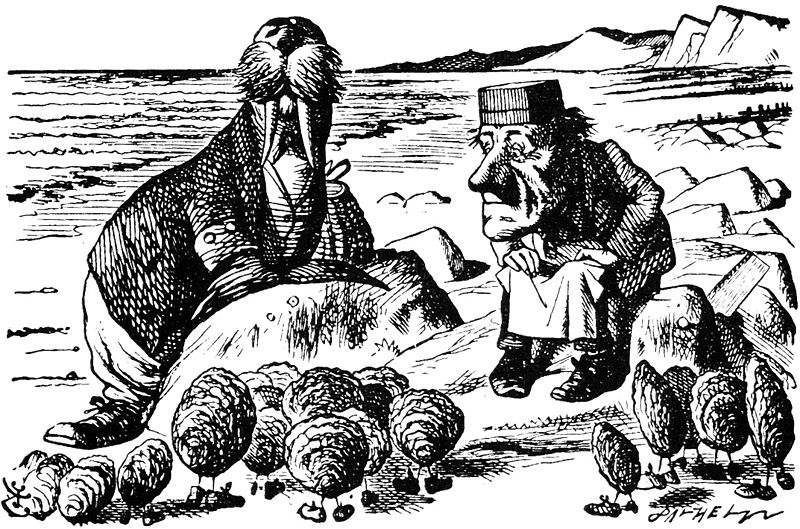
\includegraphics{photo.old/800px-Briny_Beach.jpg}
% \end{center}
% \caption[Poem]{The Walrus and the Carpenter}
% \label{fig:walrus}
% \end{figure}

\section{ภาพรวมของแอพพลิเคชัน}

% เว็บแอพพลิเคชันจะเป็นแบบ three-tier architecture แต่ว่าจะทำการออกแบบ และพัฒนาให้สามารถรองรับการเปลี่ยนแปลงเป็น 
% microservice ได้ โดย Front-end และ Back-end ส่วนมากจะพัฒนาด้วย Next.js และ tRPC เพื่อความสะดวกสบายในการเรียกใช้งาน API
% และใช้ typescript ให้มีประสิทธิภาพ แต่ Back-end ในส่วนของระบบจับคู่นั้นจะพัฒนาด้วย Go เพราะสามารถเขียน concurrency ได้ง่ายแต่ยังคงไว้ซึ่งประสิทธิภาพ
% ส่วนสุดท้ายคือฐานข้อมูลจะใช้ postgresql ในการจัดเก็บและติดต่อกับ Back-end ทั้ง Next.js และ Go

เว็บแอพพลิเคชันจะเป็นแบบ three-tier architecture แต่จะทำการออกแบบและพัฒนาให้สามารถรองรับการเปลี่ยนแปลงเป็น microservice ได้โดย 
frontend และ backend จะพัฒนาด้วย Next.js ,TypeScript และ tRPC ซึ่งมีส่วนช่วยให้การพัฒนามีความถูกต้องจากตัวแปรของทั้ง backend และ 
frontend เพราะอัลกอริทึมมีอินพุตที่ต้องการเป็นจำนวนมาก และมีหลายส่วนย่อยเมื่อมีการเรียกใช้งานข้ามไปมา ถ้าไม่มีการจำกัดประเภทตัวแปรที่ต้องส่งจะทำให้เกิดข้อผิดพลาดเป็นจำนวนมาก
ส่วนสุดท้ายคือฐานข้อมูลจะใช้ PostgreSQL ในการจัดเก็บและติดต่อกับ backend

% เว็บแอพพลิเคชันใช้ three-tier architecture~\cite{ttarch} ในการออกแบบระบบ โดย front-end ใช้ Next.js\cite{nextjs} 
% ที่เป็น React~\cite{react} framework ส่วน back-end ใช้ Gin Gonic~\cite{gingonic} ซึ่งเป็น Go~\cite{golang} framework ติดต่อกับ Front-end 
% ด้วย GraphQL~\cite{graphql} API และฐานข้อมูลใช้ MySQL~\cite{mysql} เป็น relational database management system (RDBMS)

\begin{figure}[ht]
  \begin{center}
    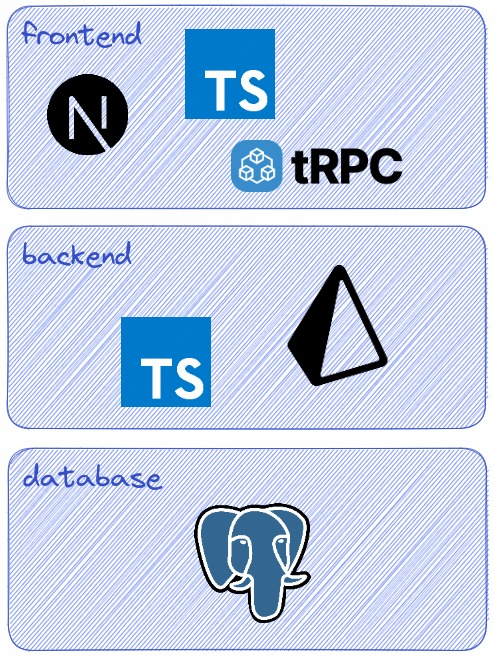
\includegraphics[width=2.5in]{photo/diagram/app-arch.jpeg}
  \end{center}
  \caption{three-tier architecture}
  \label{fig:three-tier}
\end{figure}

\section{ขั้นตอนการจับคู่}
% ในส่วนของกระบวนการจับคู่นั้น จะแบ่งออกเป็น 3 ขั้นตอนนั่นคือ การระบุความต้องการของผู้ร่วมอาศัย การให้นิยามความคล้ายคลึงกันของรายการความต้องการ
% และการจับคู่ผู้ร่วมอาศัยตามความต้องการ
การจับคู่หารูมเมทที่คู่ควรนั้น โครงการนี้ได้แบ่งขั้นตอนไว้ ด้วยกันทั้งสิ้น 3 ส่วนด้วยกัน นั่นคือ
\begin{enumerate}
  \item preference declaration: การระบุ preference ของรูมเมทหรือห้องที่ต้องการ และ profile ของเจ้าของ preference นั้น 
  \item finetuning: การหาขอบเขตลักษณะของรูมเมทที่พอรับได้ และน้ำหนักความสนใจของแต่ละคุณลักษณะของรูมเมท
  \item matching: การจับคู่จะพิจารณาจากข้อมูลที่ได้ในขั้นตอนที่ $1$ และ $2$
\end{enumerate}

\begin{figure}[ht]
  \begin{center}
    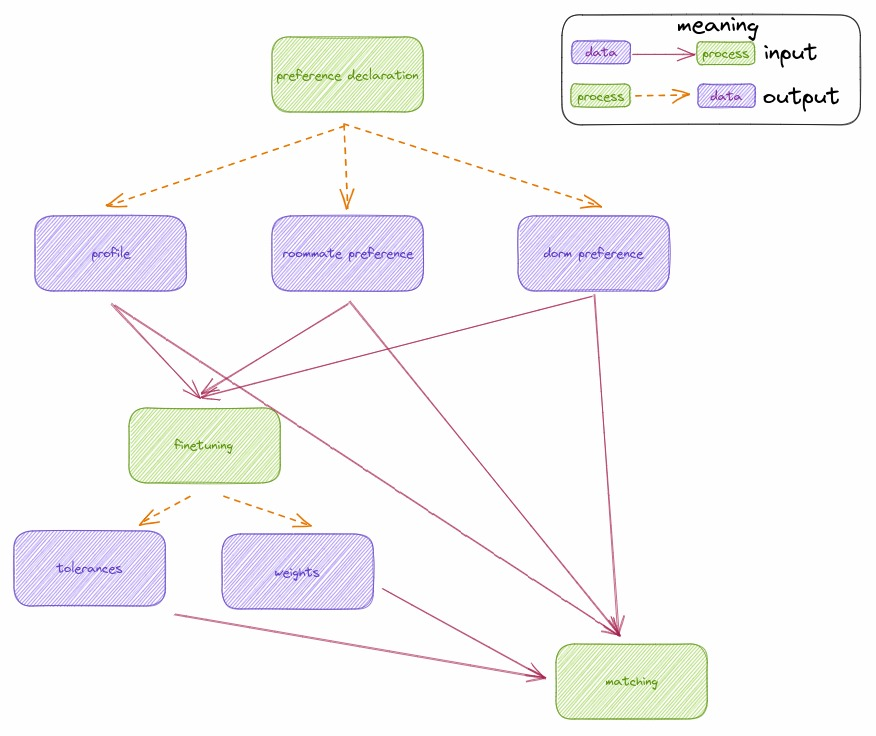
\includegraphics[width=\linewidth]{photo/diagram/matching-flow.jpeg}
  \end{center}
  \caption{ภาพรวมของอัลกอริทึม}
  \label{fig:match-overall}
\end{figure}

\subsection{ระบุรายการความต้องการ}
ในขั้นแรกของอัลกอริทึมจะทำการรวบรวมข้อมูลต่างๆ ของผู้ใช้ได้แก่ 
คุณลักษณะของผู้ใช้ คุณลักษณะของผู้ร่วมอาศัยที่ต้องการ ห้องพักที่ต้องการ หอพักที่ต้องการ เรียกว่า $\mathit{profile}$, $\mathit{matePref}$, $\mathit{roomPref}$,
และ $\mathit{dormPref}$ ตามลำดับ

\subsection{คำนวณขอบเขตลักษณะของรูมเมทที่พอรับได้}
หลังจากที่ได้ preference ต่างๆ ครบถ้วนแล้ว จะทำการค้นหาขอบเขตลักษณะของรูมเมท (tolerances) ที่เจ้าของระบุมา
เนื่องจากอัลกอริทึมนี้ตั้งสมมุติฐานไว้ว่าผู้ใช้นั้นไม่ได้รู้ถึงความต้องการที่แน่ชัดของตนเอง เช่น 
นาย ก บอกว่าอยากได้รูมเมทที่มีการรักษาความสะอาดระดับ 4 ซึ่งจริงๆแล้ว อาจจะยอมรับระดับ 5 ได้ หรืออาจจะไม่ยอมรับรูมเมทที่รักษาความสะอาดมากกว่าตัวเองเช่นระดับ 1
โดยวิธีการให้ผู้ใช้เลือกโปรไฟล์ที่มีการปรับค่าคุณลักษณะแล้วให้เจ้าของ preference เลือกว่าโปรไฟล์ไหนที่ต้องการบ้างด้วยเช่นเจ้าของ preference ระบุว่าต้องการ $messiness$ เท่ากับ 5
อัลกอริทึมจะสร้างโปรไฟล์ที่ $messiness$ มีค่า 7 มาให้เลือกซึ่งถ้าโปรไฟล์ไม่ถูกเลือกจะสร้างโปรไฟล์ที่ $messiness$ มีค่าเท่ากับ 6 มาให้ ถ้าโปรไฟล์นั้นถูกเลือกก็จะได้ว่ามีค่า $tolerant_{max}$ เท่ากับ 6
ซึ่งจริงๆ แล้วก็คือการปรับโดยใช้ binary search ดังรูปตัวอย่างที่ \ref{fig:tolerance-binary}
\begin{figure}[ht]
  \begin{center}
    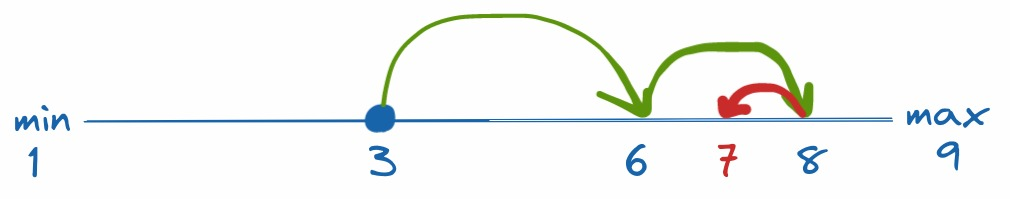
\includegraphics[width=\linewidth]{photo/diagram/binary_tolerance.jpeg}
  \end{center}
  \caption{ตัวอย่างการหา $\mathit{tolerance_\mathit{max}}$}
  \label{fig:tolerance-binary}
\end{figure}

\subsection{คำนวณน้ำหนักความสนใจของแต่ละคุณลักษณะของรูมเมท}
เพราะผู้ใช้แต่ละคนนั้นมีความสนใจที่แตกต่างกัน บางคนอาจจะสนใจระดับเสียงที่ใช้ในห้องพักมากที่สุด บางคนอาจจะสนใจระดับความสะอาดของรูมเมทมากที่สุด 
จึงต้องทำการค้นหาค่าน้ำหนักที่จะระบุความสำคัญของแต่ละคุณลักษณะของ preference ที่ผู้ใช้ระบุ ว่าผู้ใช้แต่ละคนมีความสนใจคุณลักษณะไหนอย่างไรบ้าง  
ซึ่งอัลกอริทึมการจับคู่จะนำข้อมูลน้ำหนัก (weights) เหล่านี้ไปใช้ประกอบการจับคู่รูมเมทในขั้นถัดไป โดยวิธีการหาค่าน้ำหนักมีดังนี้
\subsubsection{สร้างโปรไฟล์ให้เจ้าของ preference}
เริ่มต้นด้วยการสร้างโปรไฟล์รูมเมทจำลองขึ้นมา 2 โปรไฟล์ที่มีการปรับแต่งลักษณะที่ต่างกัน แล้วให้เจ้าของ preference เลือก 
โดยการสร้างโปรไฟล์สมมุติของรูมเมท จะทำการสุ่มเลือกคู่ของลักษณะที่ต้องการเปรียบเทียบ $(\mathit{attr}_1, \mathit{attr}_2)$ หลังจากนั้นจะใช้ข้อมูล 
$\mathit{matePref}$ และ tolerances ของเจ้าของในการสร้างโปรไฟล์สมมุติตามคุณสมบัติที่ทำการสุ่มมาได้ เช่น สุ่มได้เป็น $(\mathit{messiness}, \mathit{loudness})$ 
ผู้ใช้ที่มี $\mathit{matePref}$ ระบุว่าต้องการรูมเมทที่มีระดับการรักษาความสะอาดที่ระดับ 3 และมี tolerances ของการรักษาความสะอาด ($\mathit{messiness}$) อยู่ที่มากสุดระดับ 2 
น้อยสุดระดับ 5 ในการสร้างจะสุ่มค่าจากช่วง 2--5 แล้วนำค่าที่สุ่มได้ไปแทนในค่าการรักษาความสะอาดในโปรไฟล์สมมุติ และเช่นเดียวกันกับการใช้เสียง ($\mathit{loudness}$)
ซึ่งจากขั้นตอนดังกล่าวจะเห็นได้ว่าโปรไฟล์ที่สร้างมานั้นผู้ใช้จะต้องเลือกแน่นอนเพราะเป็นโปรไฟล์ที่อยู่ในช่วงค่าที่รับได้อย่างแน่นอน หาก ณ เวลานั้นเจ้าของ preference 
ยังคงไม่มีการเปลี่ยนแปลงคุณลักษณะรูมเมทที่ต้องการ

\subsubsection{เลือกโปรไฟล์}
หลังจากสร้างโปรไฟล์เสร็จสิ้นจะให้เจ้าของ preference นั้นเลือกโปรไฟล์ที่ต้องการอยากได้มากกว่า ซึ่งนั่นหมายความว่าอีกโปรไฟล์นั้นมีน้ำหนักของคุณลักษณะที่เปลี่ยนสูงกว่าโปรไฟล์ที่เลือก
ตัวอย่างดังรูปที่ \ref{fig:weight-adjust} เจ้าของ preference ในรูปทำการเลือกโปรไฟล์ที่มีการเพิ่มค่า $\mathit{loudness}$ ไป 3 ระดับ และโปรไฟล์ที่ไม่ถูกเลือกมีการเพิ่ม $\mathit{messiness}$ ไป 2 ระดับ
ซึ่งจะหมายความว่าการที่ $\mathit{messiness}$ เพิ่มไป 2 นั้นทำให้เจ้าของไม่พึงพอใจมากกว่าการที่ $\mathit{loudness}$ เพิ่มไป 3 กล่าวคือ $\mathit{messiness}$ นั้นมี weight ที่มากกว่า $\mathit{loudness}$
ดังนั้นอัลกอริทึมจะต้องทำการปรับ weight ของ $\mathit{loudness}$ ลง

\begin{figure}[p]
  \begin{center}
    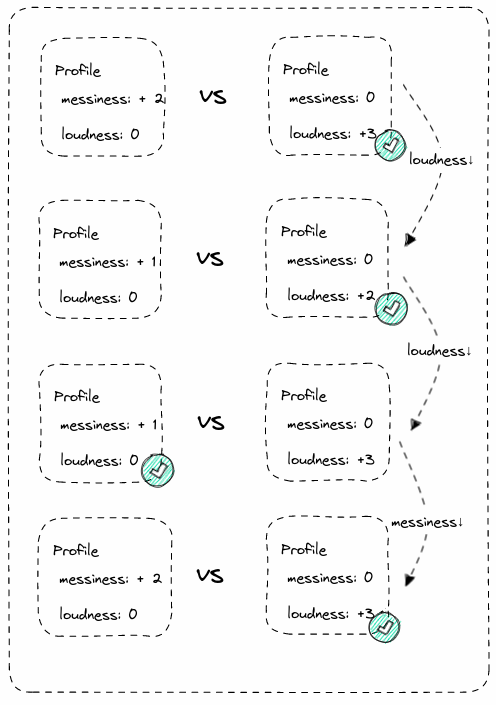
\includegraphics[width=\linewidth]{photo/diagram/weight_adjustment.png}
  \end{center}
  \caption{การปรับเปลี่ยนค่าน้ำหนักจากการเลือกโปรไฟล์}
  \label{fig:weight-adjust}
\end{figure}

\subsubsection{วิธีการคำนวณ penalty}
หลังจากทราบ weight ที่ต้องการปรับลดแล้ว การจะทราบได้ว่า weight จะต้องลดไปเท่าใดนั้นต้องมีค่าที่ใช้เปรียบเทียบ ซึ่งในที่นี้จะใช้ penalty
ซึ่งเป็นค่าที่ใช้บ่งบอกว่า โปรไฟล์รูมเมทคนดังกล่าวนั้นมีความเหมาะสมกับ preference ที่พิจารณามากน้อยเพียงใด
โดยค่า penalty มีอยู่ทั้งสิ้น 2 แบบ ได้แก่
\begin{enumerate}
  \item $\mathit{penalty}_\mathit{attr}$ คือค่าความแตกต่างของ attribute หนึ่งๆ เช่น $\mathit{messiness}$ และ $\mathit{loudness}$ ระหว่างโปรไฟล์กับ preference ซึ่งจะนำไปใช้ในการปรับค่า $\mathit{weight}_\mathit{attr}$
  \item $\mathit{penalty}_\mathit{all}$ คือผลรวมของ $\mathit{penalty}_\mathit{attr}$ จากทุกๆ atrributes ซึ่งจะนำไปใช้คิดหาความเหมาะสมของทั้งโปรไฟล์ในการจับคู่
\end{enumerate}

ในการคำนวณค่า $\mathit{penalty}_\mathit{attr}$ นั้นจำเป็นต้องใช้ข้อมูล 2 ส่วน คือค่า $\mathit{weight}_\mathit{attr}$ และ $\Delta \mathit{attr}$ โดยที่
\begin{enumerate}
  \item $\mathit{weight}_\mathit{attr}$ คือ weight ของ attribute ที่สนใจ $\mathit{attr}$
  \item $\Delta \mathit{attr} = |\mathit{attr}_\mathit{profile} -\mathit{attr}_\mathit{roomPref}|$ (ผลต่างระหว่างค่าคุณลักษณะของโปรไฟล์รูมเมทกับค่าคุณลักษณะของรูมเมทที่เราสนใจ)
\end{enumerate}
ซึ่งการจะปรับ $\mathit{weight}_\mathit{attr}$ นั้นต้องอ้างอิงจากข้อจำกัดที่ว่า หากปรับค่า weight ใหม่แล้ว ค่า penalty ของ profile ที่ถูกเลือก (เรียกว่า
$\mathit{penalty'}_\mathit{attr\_picked}$) จะต้องน้อยกว่าค่า penalty ที่คำนวณจาก ของ profile ที่ไม่ได้ถูกเลือก (เรียกว่า
$\mathit{penalty'}_\mathit{attr\_unpicked}$) ซึ่งก็คืออสมการ
\begin{equation}
  \mathit{penalty'}_\mathit{attr\_picked} < \mathit{penalty'}_\mathit{attr\_unpicked}
\end{equation}
%
โดยการที่เรากำลังจะปรับลดค่า $\mathit{weight'}_\mathit{attr\_picked}$ นั้นทำให้ทราบว่าค่า penalty ใหม่ของทั้งโปรไฟล์ที่ไม่ถูกเลือก
(เรียกว่า $\mathit{penalty'_\mathit{all\_unpicked}}$) นั้นมีค่าน้อยกว่า ค่า penalty เก่าของทั้งโปรไฟล์ที่ไม่ถูกเลือก(เรียกว่า $\mathit{penalty_\mathit{all\_unpicked}}$) ดังอสมการ
\begin{equation}
  \mathit{penalty'_\mathit{all\_picked}} < \mathit{penalty_\mathit{all\_unpicked}}
\end{equation}
%
เมื่อขยายพจน์ออกมาจะได้ดังอสมการ
\begin{equation}
  \sum_{\mathit{attr\_picked} = 1}^{n} \mathit{penalty_\mathit{attr\_picked}} 
  < \sum_{\mathit{attr\_unpicked} = 1}^{n} \mathit{penalty_\mathit{attr\_unpicked}}
\end{equation}
โดยที่
\begin{align}
  \sum_{\mathit{attr} = 1}^{n} \mathit{penalty_\mathit{attr\_picked}} &= 
  \mathit{weight'_\mathit{attr1}} \Delta\mathit{attr1_\mathit{picked}} 
  + \mathit{weight_\mathit{attr2}} \Delta\mathit{attr2_\mathit{picked}} \\
  \sum_{\mathit{attr} = 1}^{n} \mathit{penalty_\mathit{attr\_unpicked}} &= 
  \mathit{weight'_\mathit{attr1}} \Delta\mathit{attr1_\mathit{unpicked}} 
  + \mathit{weight_\mathit{attr2}} \Delta\mathit{attr2_\mathit{unpicked}}
\end{align}
%
จัดรูปใหม่จะได้ว่า
\begin{equation}
  \mathit{weight'_\mathit{attr1}} 
  (\Delta\mathit{attr1_\mathit{picked}} - \Delta\mathit{attr1_\mathit{unpicked}})
  < \mathit{weight_\mathit{attr2}} 
  (\Delta\mathit{attr2_\mathit{unpicked}} - \Delta\mathit{attr2_\mathit{picked}})
\end{equation}
%
ทำให้ทราบว่าท้ายที่สุดแล้วค่า $\mathit{weight'_\mathit{attr1}}$ หรือก็คือ $\mathit{weight'_\mathit{attr\_picked}}$ 
มีค่าดังอสมการ
\begin{equation}
  \mathit{weight'_\mathit{attr1}} 
  < \mathit{weight_\mathit{attr2}} 
  \frac{|\Delta\mathit{attr2_\mathit{unpicked}} - \Delta\mathit{attr2_\mathit{picked}}|}{|\Delta\mathit{attr1_\mathit{picked}} - \Delta\mathit{attr1_\mathit{unpicked}}|}
\end{equation}
แต่จากการที่อัลกอริทึมทำการสร้างโปรไฟล์ที่ปรับแต่งแค่ 1 ลักษณะจาก preference ต่อ 1 โปรไฟล์ดังตัวอย่างในรูปที่ \ref{fig:weight-adjust} หมายความว่าค่า
$\Delta\mathit{attr2_\mathit{picked}}$ และ $\Delta\mathit{attr1_\mathit{unpicked}}$ มีค่าเป็น 0 ดังอสมการ
\begin{equation}
  \mathit{weight'_\mathit{attr1}} 
  < \mathit{weight_\mathit{attr2}} 
  \frac{\Delta\mathit{attr2_\mathit{unpicked}}}{\Delta\mathit{attr1_\mathit{picked}}}
\end{equation}
ซึ่งก็คืออสมการ
\begin{equation}
  \mathit{weight'_\mathit{attr\_picked}} 
  < \mathit{weight_\mathit{attr\_unpicked}} 
  \frac{\Delta\mathit{attr_\mathit{unpicked}}}{\Delta\mathit{attr_\mathit{picked}}}
\end{equation}
หรือ
\begin{equation}
  \mathit{weight'_\mathit{attr\_picked}} 
  < \frac{penalty_\mathit{attr\_unpicked}}
  {\Delta\mathit{attr_\mathit{picked}}}
  \label{equa:weight-max}
\end{equation}
โดยที่
\begin{equation}
  \mathit{penalty_\mathit{attr\_unpicked}} = \mathit{weight_\mathit{attr\_unpicked}} \Delta\mathit{attr_\mathit{unpicked}}
\end{equation}
จากอสมการ \ref{equa:weight-max} ทำให้ทราบค่าขอบบนของ $\mathit{weight'_\mathit{attr\_picked}}$ 
(เรียกว่า $\mathit{weight'}_\mathit{max}$) ดังนั้นเพื่อความง่ายจึงใช้ขอบล่างของ $\mathit{weight'_\mathit{attr\_picked}}$ 
(เรียกว่า $\mathit{weight'}_\mathit{min}$) ดังสมการ
\begin{equation}
  \mathit{weight'}_\mathit{min} = \frac{\mathit{penalty}_\mathit{attr\_unpicked}}{\Delta \mathit{attr}_\mathit{picked} + 1}
\end{equation}
%
ดังนั้นจากข้อมูลข้างต้นเราจะสามารถคำนวณช่วงของค่า $\mathit{weight'}_\mathit{attr\_picked}$ ที่เป็นไปได้ ดังอสมการ
\begin{equation}
  \mathit{weight'}_\mathit{min}
  < \mathit{weight'}_\mathit{attr\_picked} 
  < \mathit{weight'}_\mathit{max} 
\end{equation}
โดยที่
\begin{align}
  \mathit{weight'}_\mathit{min} &= \frac{\mathit{penalty}_\mathit{attr\_unpicked}}{\Delta \mathit{attr}_\mathit{picked} + 1} \\
  \mathit{weight'}_\mathit{max} &= \frac{\mathit{penalty}_\mathit{attr\_unpicked}}{\Delta \mathit{attr}_\mathit{picked}}
\end{align}
หลังจากทราบข้อจำกัดข้างต้นแล้ว เราจะกำหนด $\mathit{weight'}_\mathit{attr\_picked}$ เป็นค่ากึ่งกลางระหว่าง $\mathit{weight'}_\mathit{min}$ 
และ $\mathit{weight'}_\mathit{max}$

\subsubsection{การนอมัลไลเซชัน weights} 
เนื่องจากค่า weights นั้นเป็นเหมือนกับ vector การแทนค่า $\mathit{weight'}_\mathit{attr\_picked}$ สับเปลี่ยนกันไปตามแต่ละคุณลักษณะซ้ำๆ 
จะทำให้ vector ของ weigths นั้นไม่ใช่ vector 1 หน่วย ส่งผลใหเ้ความหมายของ weight แต่ละค่านั้นไม่สมจริง จึงต้องทำการนอมัลไลเซชัน
เพื่อให้ weights คำนวณได้ง่าย ซึ่งจะใช้ L2 นอมัลไลเซชันในการคำนวณ ดังสมการ
\begin{align}
  \mathit{weights} &= [\mathit{weight}_\mathit{messiness}, \mathit{weight}_\mathit{loudness}, \mathit{weight}_\mathit{do\_not\_disturb}] \\
  \mathit{magnitude} &= \sqrt{\mathit{weight}_\mathit{messiness}^2 + \mathit{weight}_\mathit{loudness}^2 + \mathit{weight}_\mathit{do\_not\_disturb}^2} \\
  \mathit{weights}_\mathit{norm} &= \mathit{weights} / \mathit{magnitude}
\end{align}

\begin{figure}[h]
  \begin{center}
    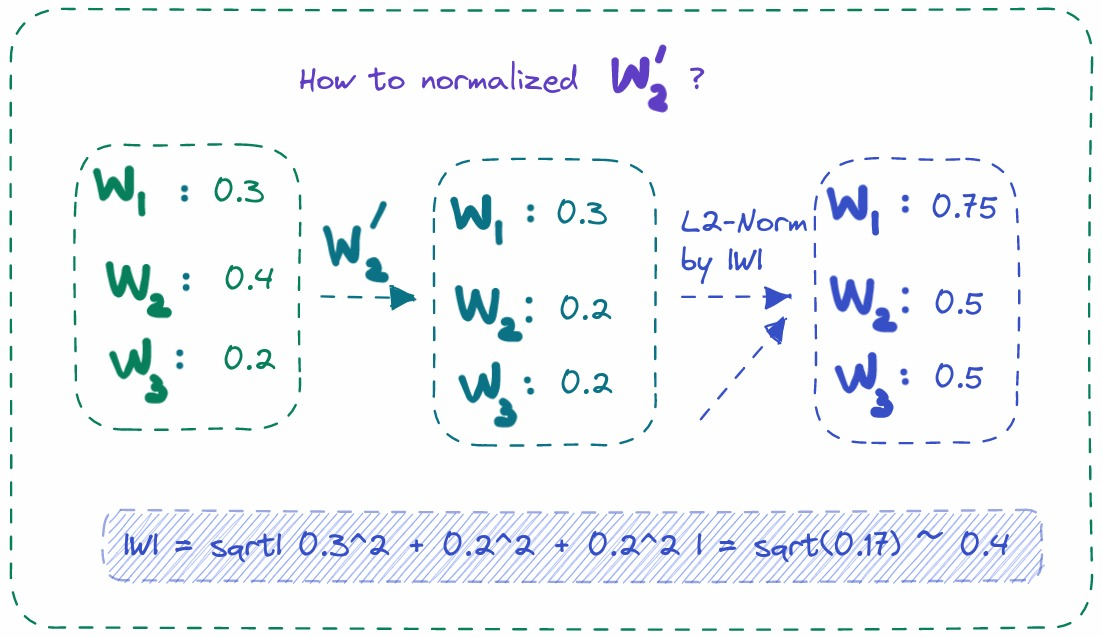
\includegraphics[width=\linewidth]{photo/diagram/weight_norm.jpeg}
  \end{center}
  \caption{ตัวอย่างการนอมัลไลเซชัน}
  \label{fig:weight-norm}
\end{figure}

หลังจากได้ $\mathit{weights}_\mathit{norm}$ เสร็จแล้วจะสามารถทำการปรับน้ำหนักซ้ำๆ ได้จนกว่าเจ้าของโปรไฟล์จะพอใจ
\begin{figure}[h]
  \begin{center}
    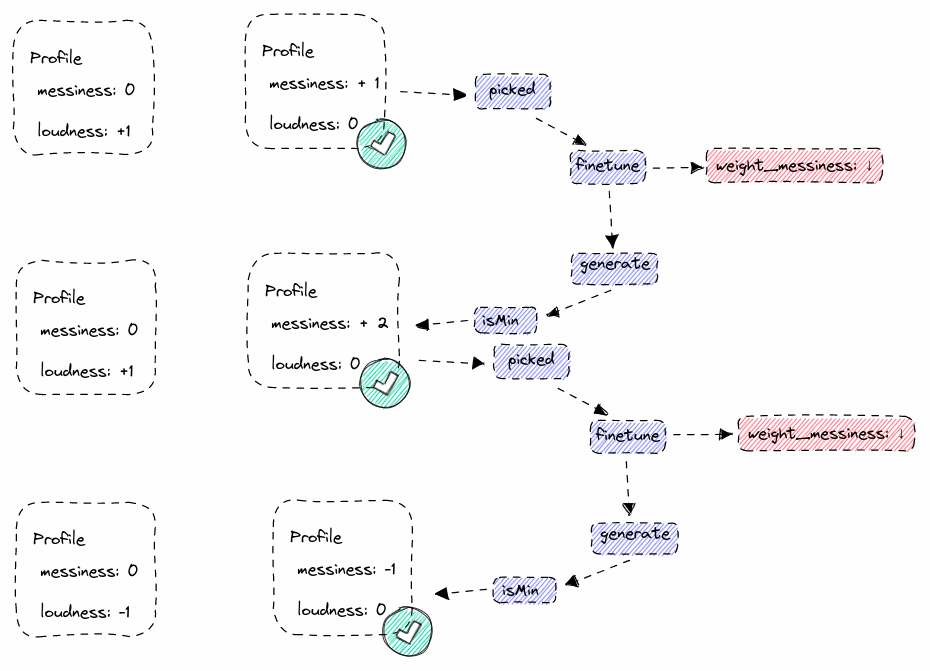
\includegraphics[width=\linewidth]{photo/diagram/finetune_flow.png}
  \end{center}
  \caption{ตัวอย่างการปรับค่า weights}
  \label{fig:finetune-flow}
\end{figure}

\subsection{วิธีตัดสินในการจับคู่ตามความต้องการ}
ระบบจะทำการคำนวณค่าบทลงโทษ(penalty) ตามคุณลักษณะที่ไม่ตรงตามความต้องการ ทำให้ผู้ใช้ที่มีคุณลักษณะไม่ตรงตามความต้องการมีค่า penalty ต่อกันสูง
โดยค่าคุณลักษณะที่จะใช้พิจารณานั้นปัจจุบันมีอยู่ทั้งสิ้น 2 แบบคือ
\begin{enumerate}
  \item แบบค่าสูงสุด คือหากคุณลักษณะมีค่าไม่เกินค่าสูงสุดค่าจะไม่มี penalty ไม่อย่างนั้นค่า penalty จะสูงขึ้นตามส่วนต่างที่เกินมาจากค่าสูงสุด
  \item แบบช่วง คือหากคุณลักษณะมีช่วงที่ซ้อนทับกับช่วงที่ต้องการพอดีจะไม่มี penalty ไม่อย่างนั้นจำนวนที่ไม่ซ้อนทับกันจะยิ่งเพิ่มค่า penalty
\end{enumerate}

\subsection{เลือกหอให้ผู้ใช้ตามความต้องการ}
ลำดับต่อไปจะเป็นการเลือกหอพักให้กับผู้ใช้ตามความต้องการ เนื่องจากหอพักนักศึกษาของมหาวิทยาลัยเชียงใหม่นั้นมีค่าใช้จ่ายที่ไม่เท่ากัน
และนักศึกษาแต่ละคนมีกำลังในการจ่ายค่าหอพักที่ไม่เท่ากัน จึงจำเป็นที่จะต้องเลือกก่อนการเลือกผู้ร่วมอาศัย 

\subsection{ตัวเลือกต่างๆ ในขั้นตอนเลือกห้องพัก และผู้ร่วมอาศัย}
เนื่องจากในส่วนก่อนหน้าที่ระบุไว้ว่าปัญหาการจับคู่นี้เป็น NP-complete จึงจำเป็นที่จะต้องหาทางเลือกอื่นในการพัฒนา 
ซึ่งสามารถแบ่งออกได้เป็น 3 แบบ ได้แก่
\begin{enumerate}
  \item เลือกผู้พักอาศัยก่อนเลือกห้องพัก
        วิธินี้จะเลือกและจัดกลุ่มของผู้พักอาศัยตามจำนวนผู้พักอาศัยใน 1 ห้องของหอพัก โดยวิธีการเลือกนั้นจะเลือกจากผู้ใช้ที่มีค่า penalty ต่อกันน้อยที่สุด
        แล้วจากนั้นแต่ละกลุ่มจะทำการเลือกห้องพักโดย penalty คิดจากผลรวมของ penalty ที่ได้จาก $\mathit{roomPref}$ ของสมาชิกในกลุ่ม
        ซึ่งวิธินี้จะทำให้นักศึกษาได้เพื่อนร่วมห้องที่ต้องการ แต่อาจจะทำให้นักศึกษาบางคนในกลุ่มไม่ได้ห้องพักตามที่ต้องการ
  \item เลือกกลุ่มของห้องพักก่อนเลือกผู้พักอาศัย
        วิธีนี้จะเลือกและจัดกลุ่มของนักศึกษาเข้าไปในกลุ่มของห้องพักก่อน โดยในแต่ละกลุ่มของห้องจะเป็นห้องที่มีลักษณะเหมือนๆกัน
        หลังจากนั้นจะทำการจับกลุ่มของนักศึกษาให้เข้ากับแต่ละห้องในกลุ่ม ซึ่งวิธีนี้จะทำให้นักศึกษาได้ห้องที่ใกล้เคียงความต้องการมากที่สุด 
        แต่จะทำให้ห้องบางห้องมีนักศึกษาที่ไม่เหมาะสมที่จะจับคู่กันเกิดขึ้น
  \item พิจารณาเลือกทั้งห้องพักและผู้พักอาศัยพร้อมๆ กัน
        วิธีนี้จะทำการคิด penalty ของทั้ง $\mathit{roomPref}$ และ $\mathit{matePref}$ พร้อมๆ กันโดยเอาค่า $\mathit{roomPref} + \mathit{matePref}$ เป็น penalty
        แต่ผู้พัฒนายังไม่สามารถหาวิธีที่จะทำการเลือกลำดับนักศึกษาที่แน่นอน ในการจับคู่ผู้ร่วมอาศัยและห้องพักพร้อมๆ กัน
\end{enumerate}

โดยวิธีพิจารณาเลือกทั้งห้องพักและผู้พักอาศัยพร้อมๆ กันนั้นยังไม่สามารถหาวิธีการที่สามารถพิสูจน์ว่าสามารถทำได้
จึงเลือกใช้วิธีเลือกผู้พักอาศัยก่อนเลือกห้องพัก เนื่องจากโครงงานนี้ต้องการให้ความสำคัญกับการเลือกรูมเมท ซึ่งวิธีการที่เลือกมาจะทำให้ผู้ใช้ได้พักอาศัยกับรูมเมทที่เหมาะสมได้ดีที่สุด
% \subsection{ตัวอย่างการทำงาน}
% \begin{enumerate}
%   \item นำลำดับคุณลักษณะที่ผู้ใช้ $u$ จัดอันดับไปแปลงเป็นตัวเลขเพื่อใช้เป็นตัวคูณในขั้นตอนต่อๆไป โดยเรียกตัวคูณนั้นว่า $\mathit{mult}$
%   \item เก็บรายการคุณลักษณะที่ผู้ใช้พิจารณาเพื่อนร่วมห้องจากการจัดลำดับในขั้นตอนก่อนหน้าแล้วเรียกว่า $\mathit{attr}$
%   \item ปรับปรุง $\mathit{mult}$ เพิ่มเติมในขั้นตอนการปรับจูน หากคุณลักษณะใดที่ผู้ใช้ให้ความสนใจบ่อยๆ จะถูกเพิ่มค่าให้มากขึ้น และคุณลักษณะใดที่ผู้ใช้ไม่ให้ความสนใจก็จะถูกลดค่าให้น้อยลง 
%         เช่น หากมีโปรไฟล์ที่มีคุณลักษณะดังนี้
%         \begin{enumerate}
%           \item เวลานอนช่วง 4 ทุ่ม -- 5 ทุ่ม และ เป็นคนช่างพูด  
%           \item เวลานอนช่วง 4 ทุ่ม -- 5 ทุ่ม และ เป็นคนพูดน้อย  
%         \end{enumerate} 
%         แล้วผู้ใช้เลือกทั้งสองโปรไฟล์นั้น ดังนั้นระบบจะทำการปรับเพิ่มค่าในตัวคูณของคุณลักษณะเวลานอนใน $\mathit{mult}$
%   \item นำ $\mathit{mult}$ ไปคูณกับค่าของคุณลักษณะของผู้ใช้ $v$ คนอื่นๆที่ไม่ใช่ $u$ แล้วบวกผลคูณทั้งหมดเข้าด้วยกัน เรียกว่า $\mathit{RoommatePref}$
%   \item ทำแบบข้อก่อนหน้ากับคุณลักษณะของห้องพักที่ต้องการ และ คุณลักษณะตามโปรไฟล์ของผู้ใช้ $u$ เรียกว่า $\mathit{RoomPref}$ และ $\mathit{PersonalPref}$ ตามลำดับ
%   \item สร้างคู่อันดับ $(\mathit{RoomPref}, \mathit{RoommatePref})$ จากค่าของผู้ใช้ เรียกว่า $(x,y)$ 
%   \item สร้างคู่อันดับ $(\mathit{RoomPref}, \mathit{PersonalPref})$ ของผู้ใช้คนอื่น เรียกว่า $(x',y')$
%   \item หาคู่อันดับ $(x',y')$ ที่มีระยะทางแบบยูคลิด~\cite{euclid-dist} จาก $(x,y)$
%   \[\sqrt{(x-x')^2 + (y-y')^2}\] มีค่าน้อยที่สุด 
%   แล้วให้ $(x',y')$ ของผู้ใช้คนนั้นคู่เป็นเพื่อนร่วมห้อง
% \end{enumerate}

\MEreply{เป็นช่วง8.1 ของ NSC อาจจะทำรูป flow คร่าวๆ}
\section{User story}
ต่อไปจะเป็นการอธิบายการทำงานของระบบในส่วนต่างๆ ทั้งฝั่งผู้ใช้งานทั่วไปและผู้ดูแลระบบ โดยรูปภาพตัวอย่างต่อไปนี้เป็นเพียง wireframes เท่านั้น ไม่ใช่ user interface ของระบบจริง
\subsection{นักศึกษา}
\begin{enumerate}
  \item นักศึกษาเข้าสู่หน้าต้อนรับของแอพพลิเคชัน แต่ยังไม่สามารถทำอะไรได้ ต้องทำการยืนยันตัวตนด้วยการคลิกปุ่ม login หรือ quick start ก่อน
        \begin{figure}[ht]
          \begin{center}
            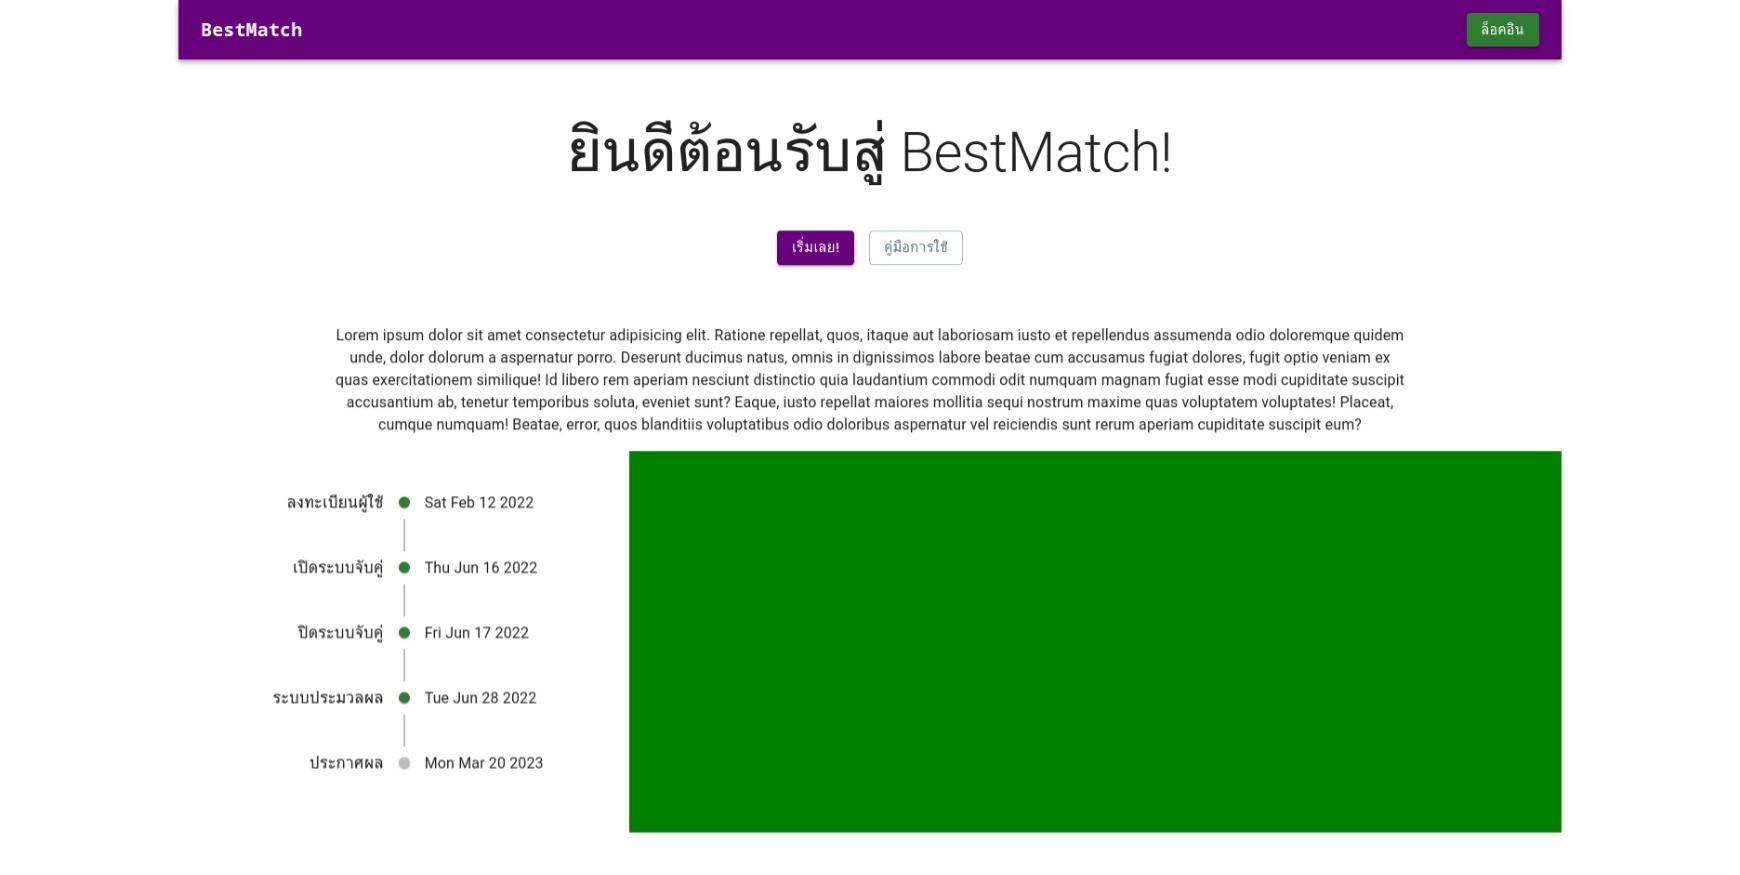
\includegraphics[width=\linewidth]{photo/web/student/home.jpeg}
          \end{center}
          \caption{หน้าต้อนรับที่ไม่ได้ยืนยันตัวตน}
          \label{fig:homepage}
        \end{figure}
        \clearpage
  \item นักศึกษายืนยันตัวตน โดยหน้าต่างล็อคอิน ซึ่งสามารถสร้างบัญชีใหม่ได้หากยังไม่มีบัญชี ดังรูปตัวอย่าง
        \begin{figure}[ht]
          \begin{center}
            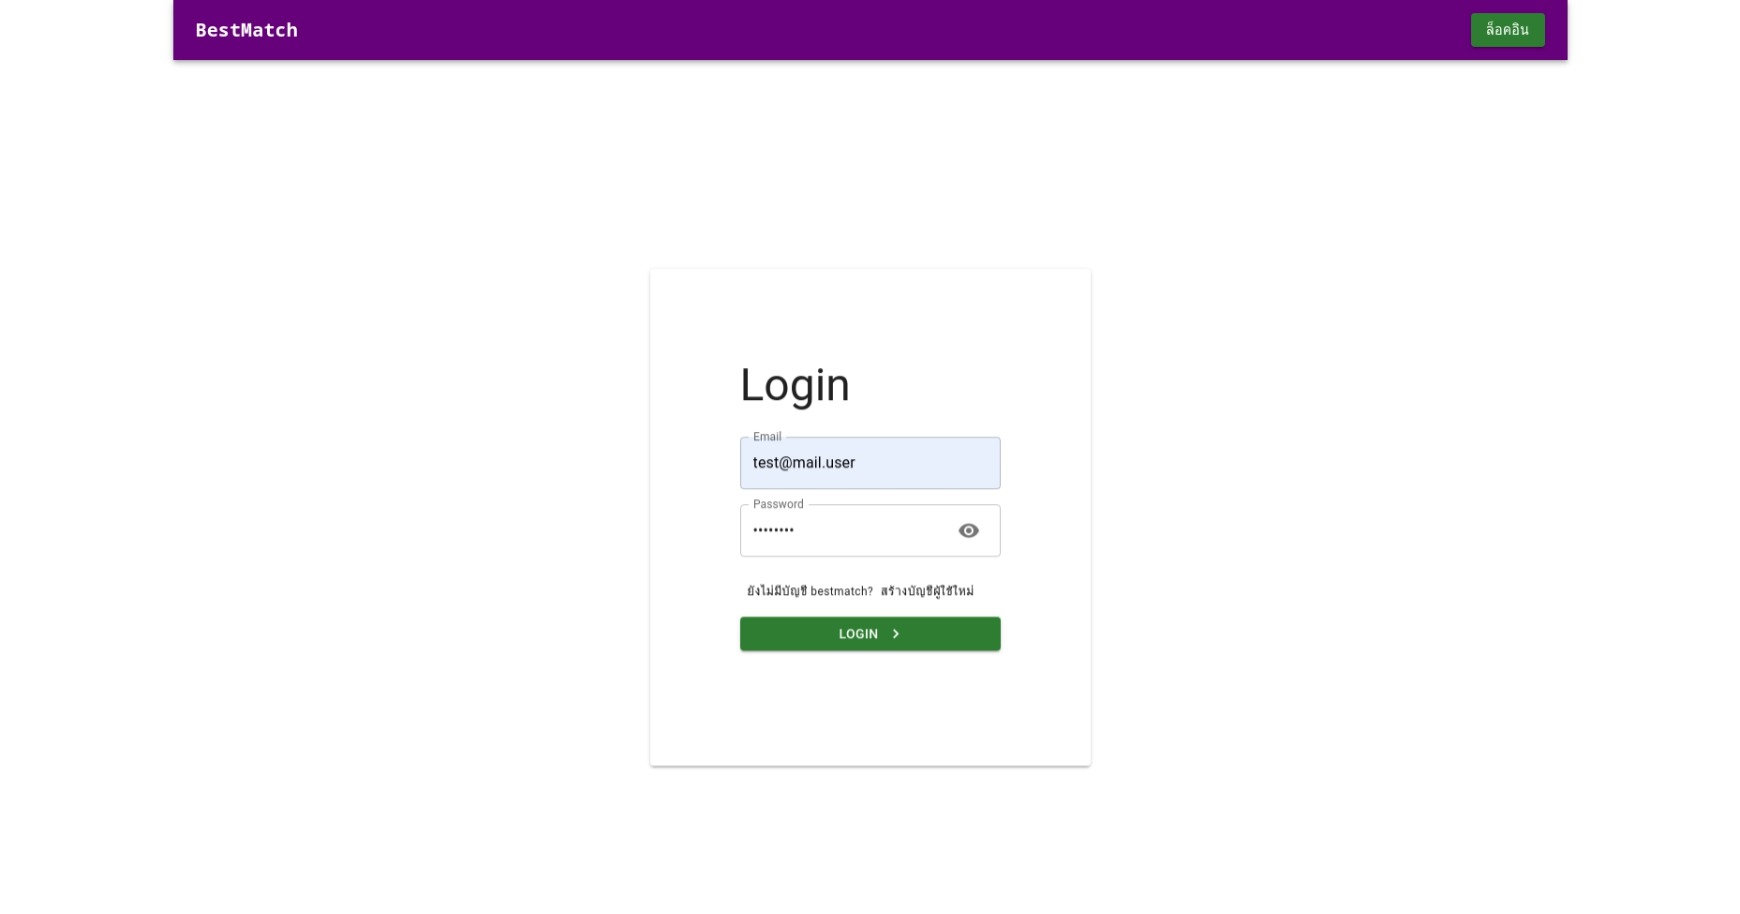
\includegraphics[width=\linewidth]{photo/web/student/login.jpeg}
          \end{center}
          \caption{หน้าต่างล็อคอิน}
          \label{fig:login}
        \end{figure}
        
        \begin{figure}[h]
          \begin{center}
            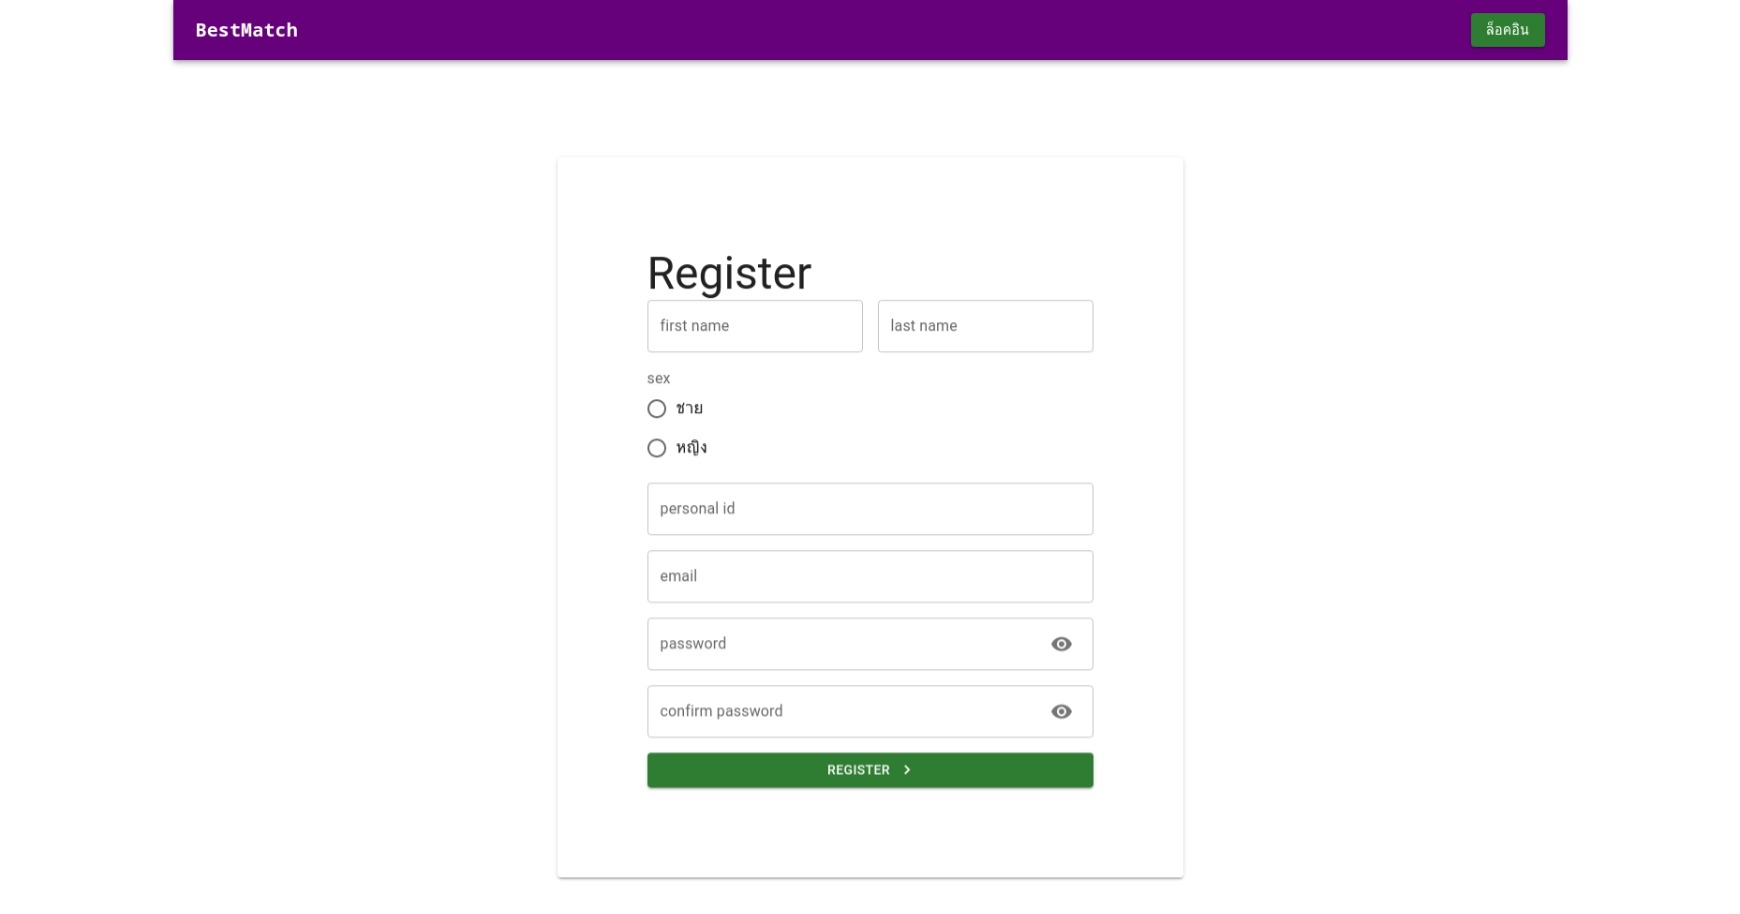
\includegraphics[width=\linewidth]{photo/web/student/register.jpeg}
          \end{center}
          \caption{หน้าต่างลงทะเบียน}
          \label{fig:register}
        \end{figure}
        
        \begin{figure}[ht]
          \begin{center}
            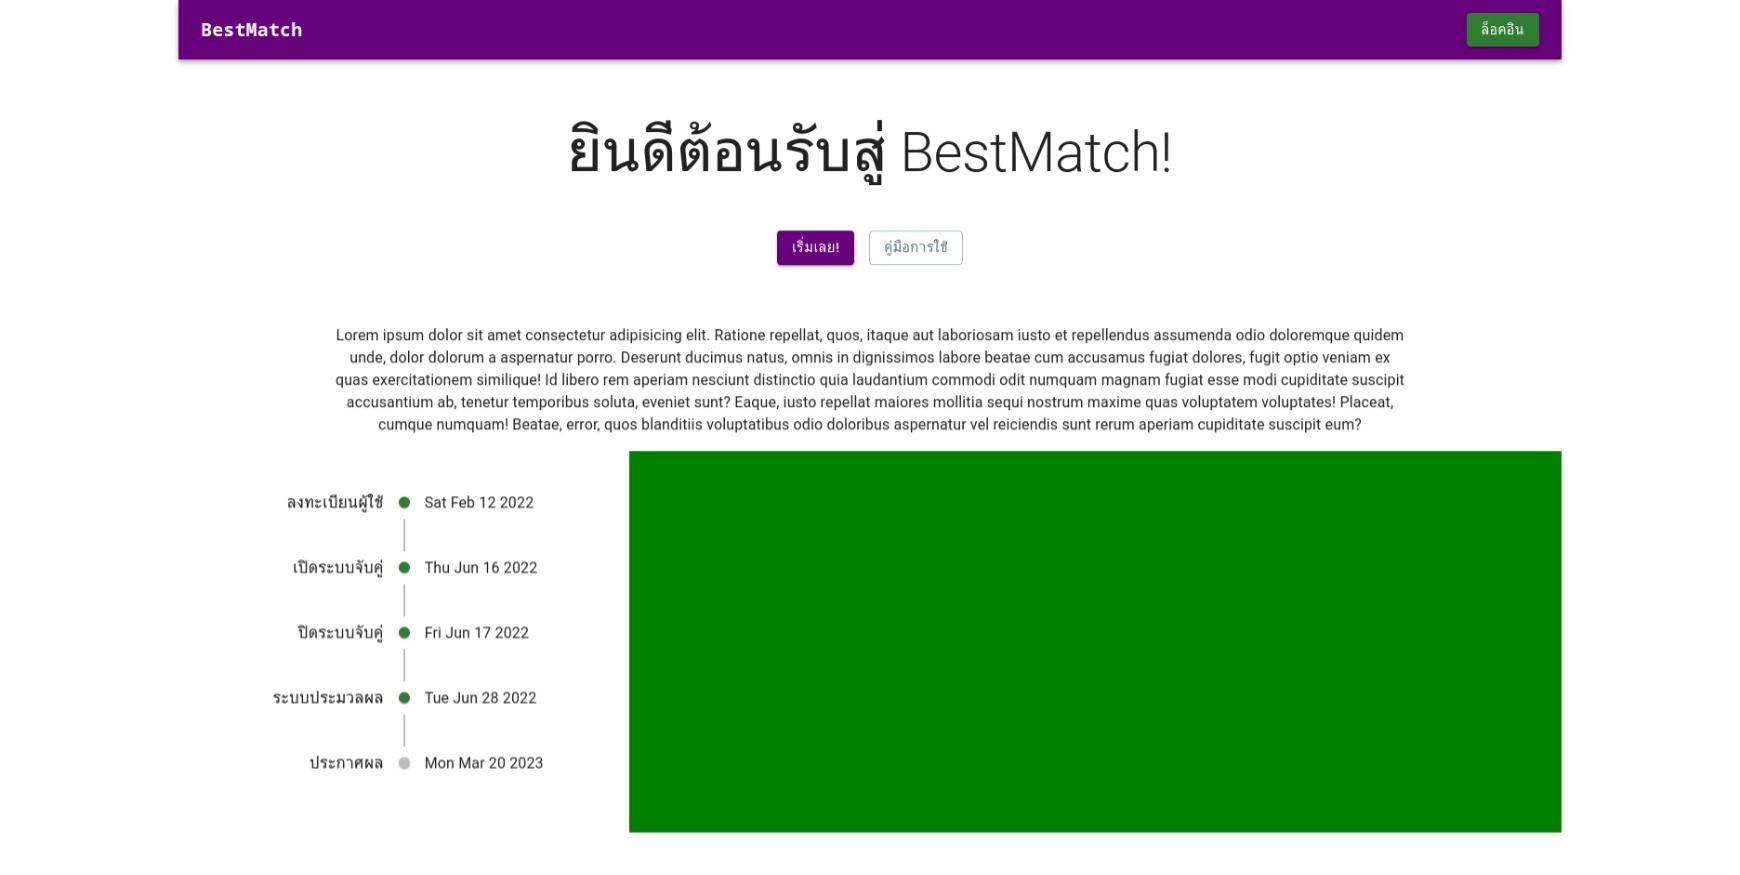
\includegraphics[width=\linewidth]{photo/web/student/home.jpeg}
          \end{center}
          \caption{หน้าต้อนรับหลังจากการยืนยันตัวตน}
          \label{fig:homepage-auth}
        \end{figure}
        \clearpage
  \item นักศึกษาเรียนรู้การทำงานด้วยหน้าต่างคู่มือการใช้งาน ซึ่งจะมีแผนผังที่สามารถมีปฏิสัมพันธ์ในการช่วยแนะนำแอพพลิเคชัน
        \begin{figure}[ht]
          \begin{center}
            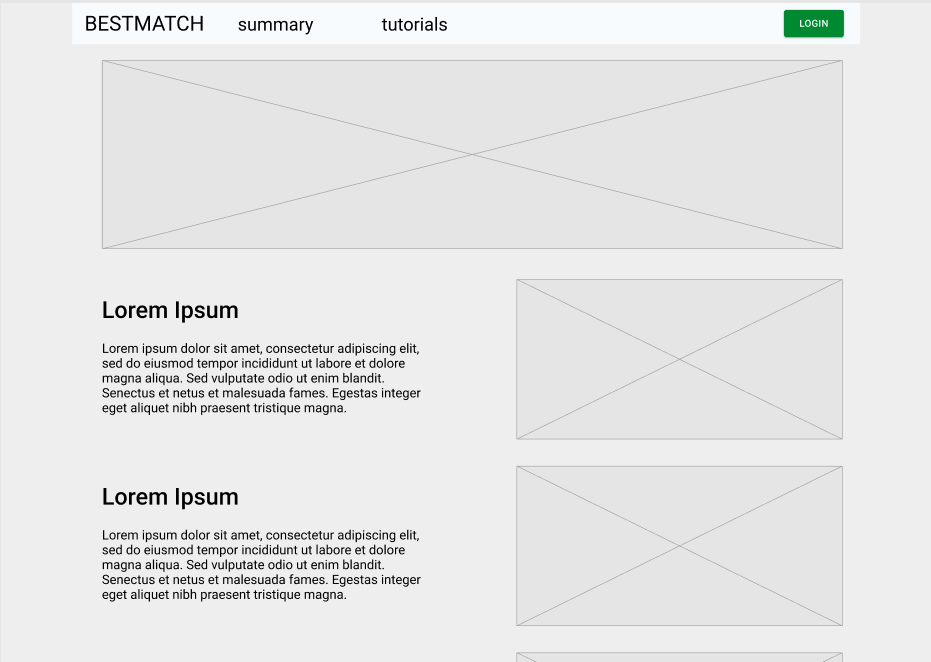
\includegraphics[width=\linewidth]{photo/student/tutorial.png}
          \end{center}
          \caption{หน้าคู่มือการใช้งาน}
          \label{fig:tutorial}
        \end{figure}
        \clearpage
  \item นักศึกษาเริ่มต้นใช้งานจะพบกับหน้าระบุคุณลักษณะของตนเอง
        \begin{figure}[ht]
          \begin{center}
            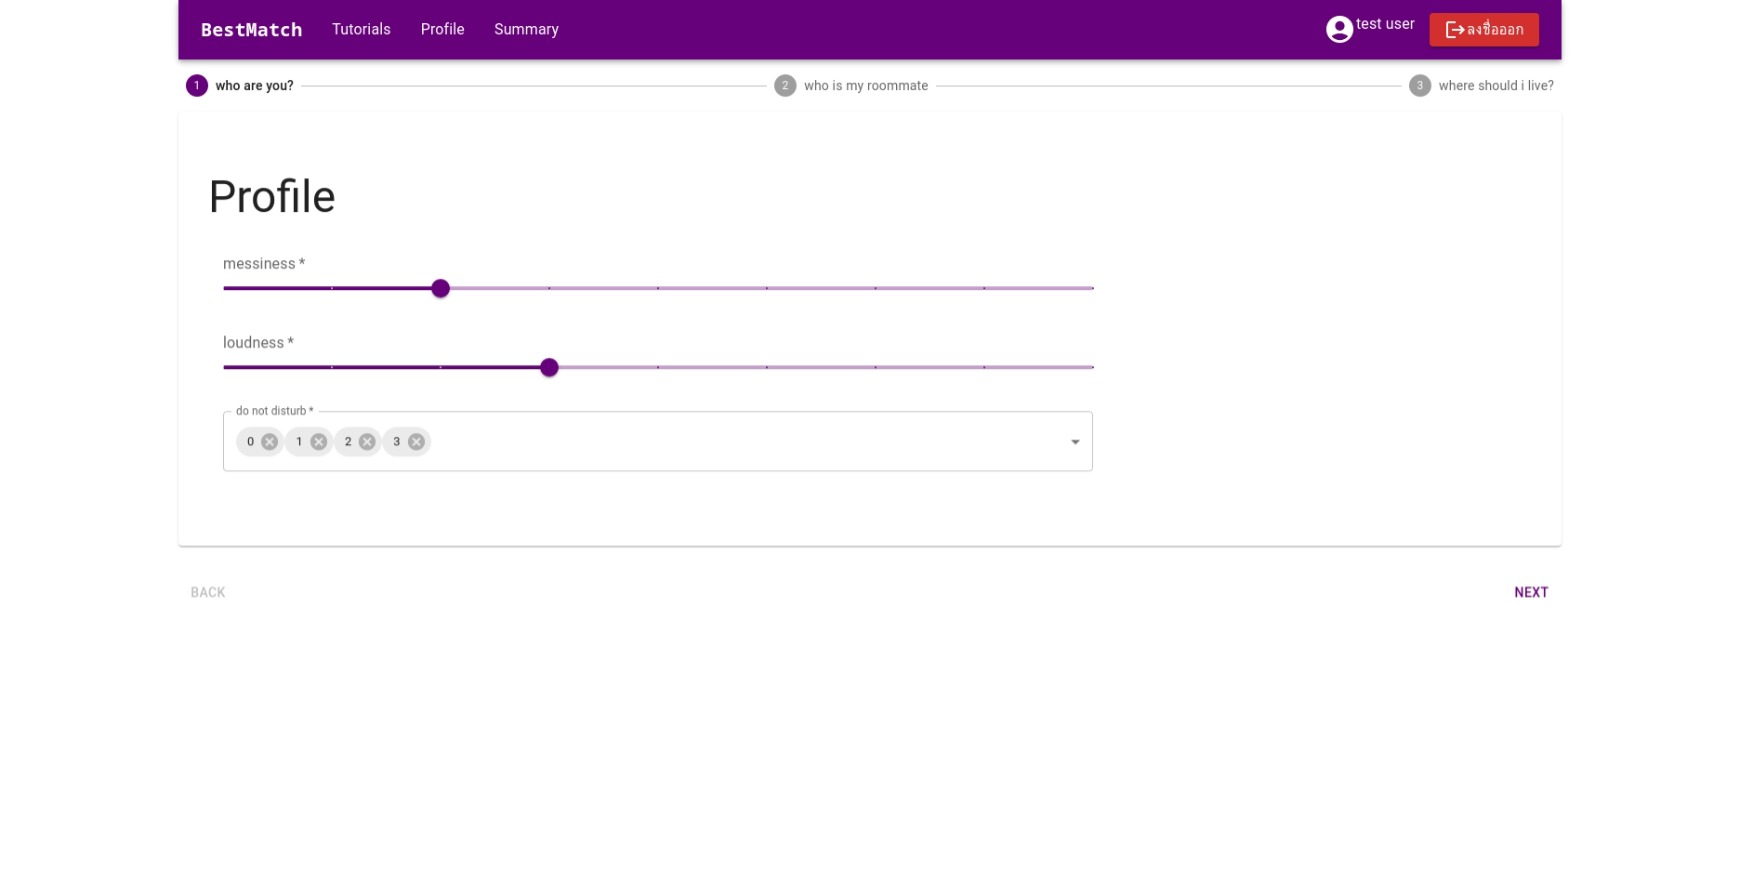
\includegraphics[width=\linewidth]{photo/web/student/profile-def.jpeg}
          \end{center}
          \caption{หน้าระบุ $\mathit{profile}$ ของนักศึกษา}
          \label{fig:user-profile}
        \end{figure}
        \clearpage
  \item นักศึกษาระบุคุณลักษณะของผู้ร่วมอาศัยที่ต้องการ
        \begin{figure}[ht]
          \begin{center}
            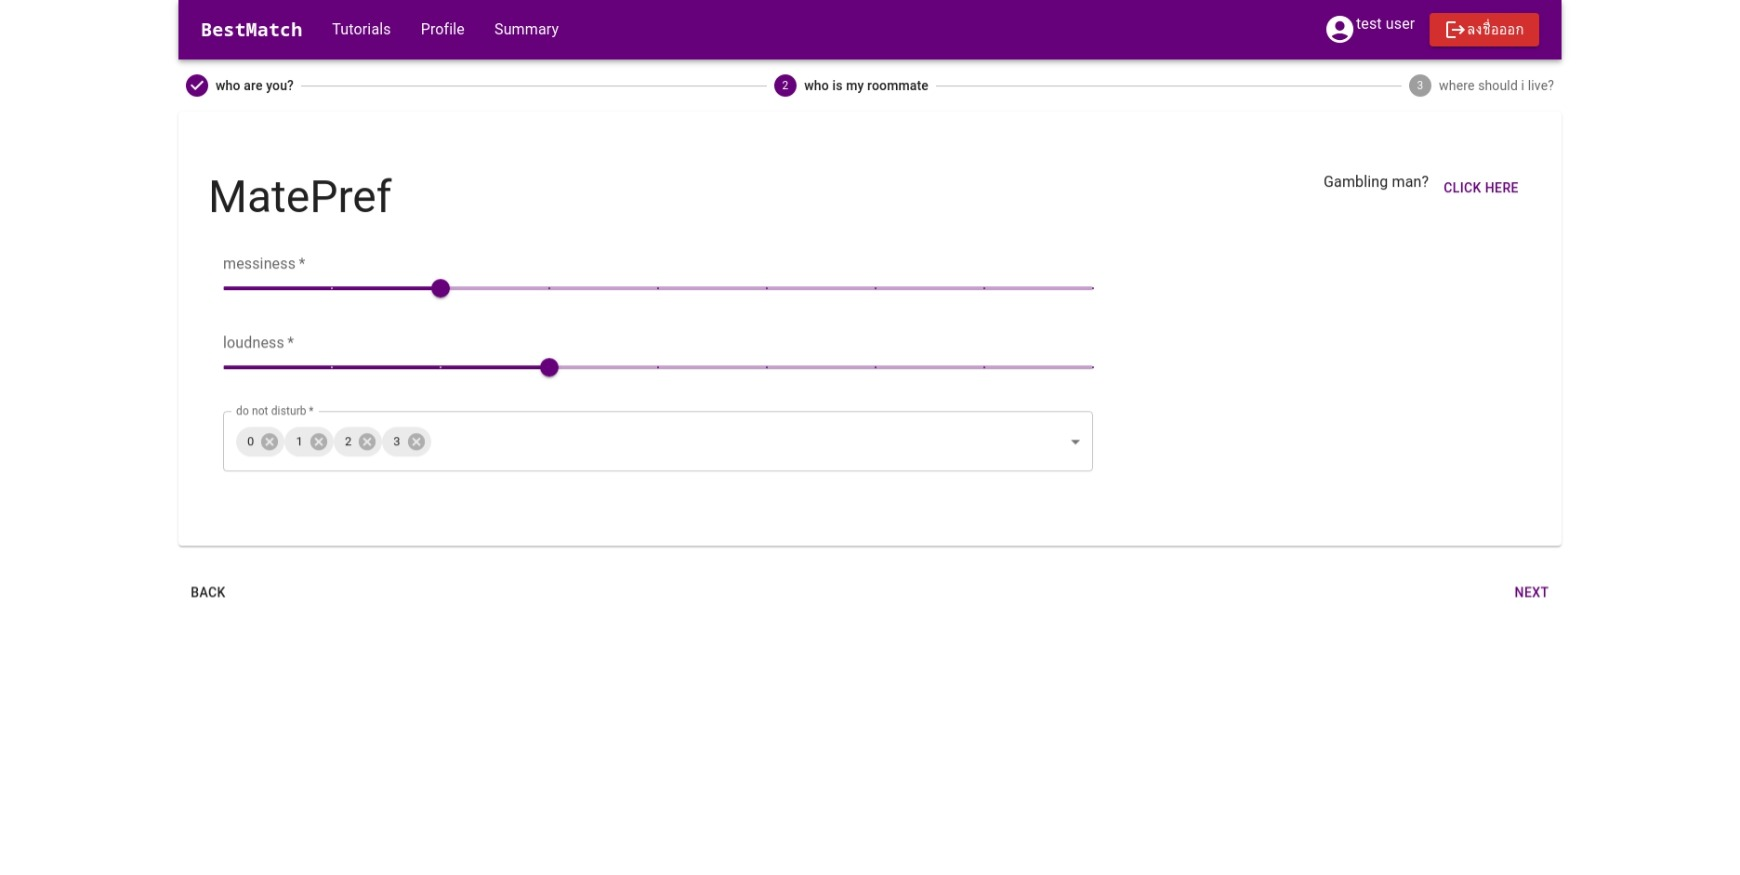
\includegraphics[width=\linewidth]{photo/web/student/mate-def.jpeg}
          \end{center}
          \caption{หน้าระบุ $\mathit{matePref}$ ของนักศึกษา}
          \label{fig:mate-pref}
        \end{figure}
        \clearpage
  \item นักศึกษาระบุห้องและหอพักที่ต้องการ
        \begin{figure}[ht]
          \begin{center}
            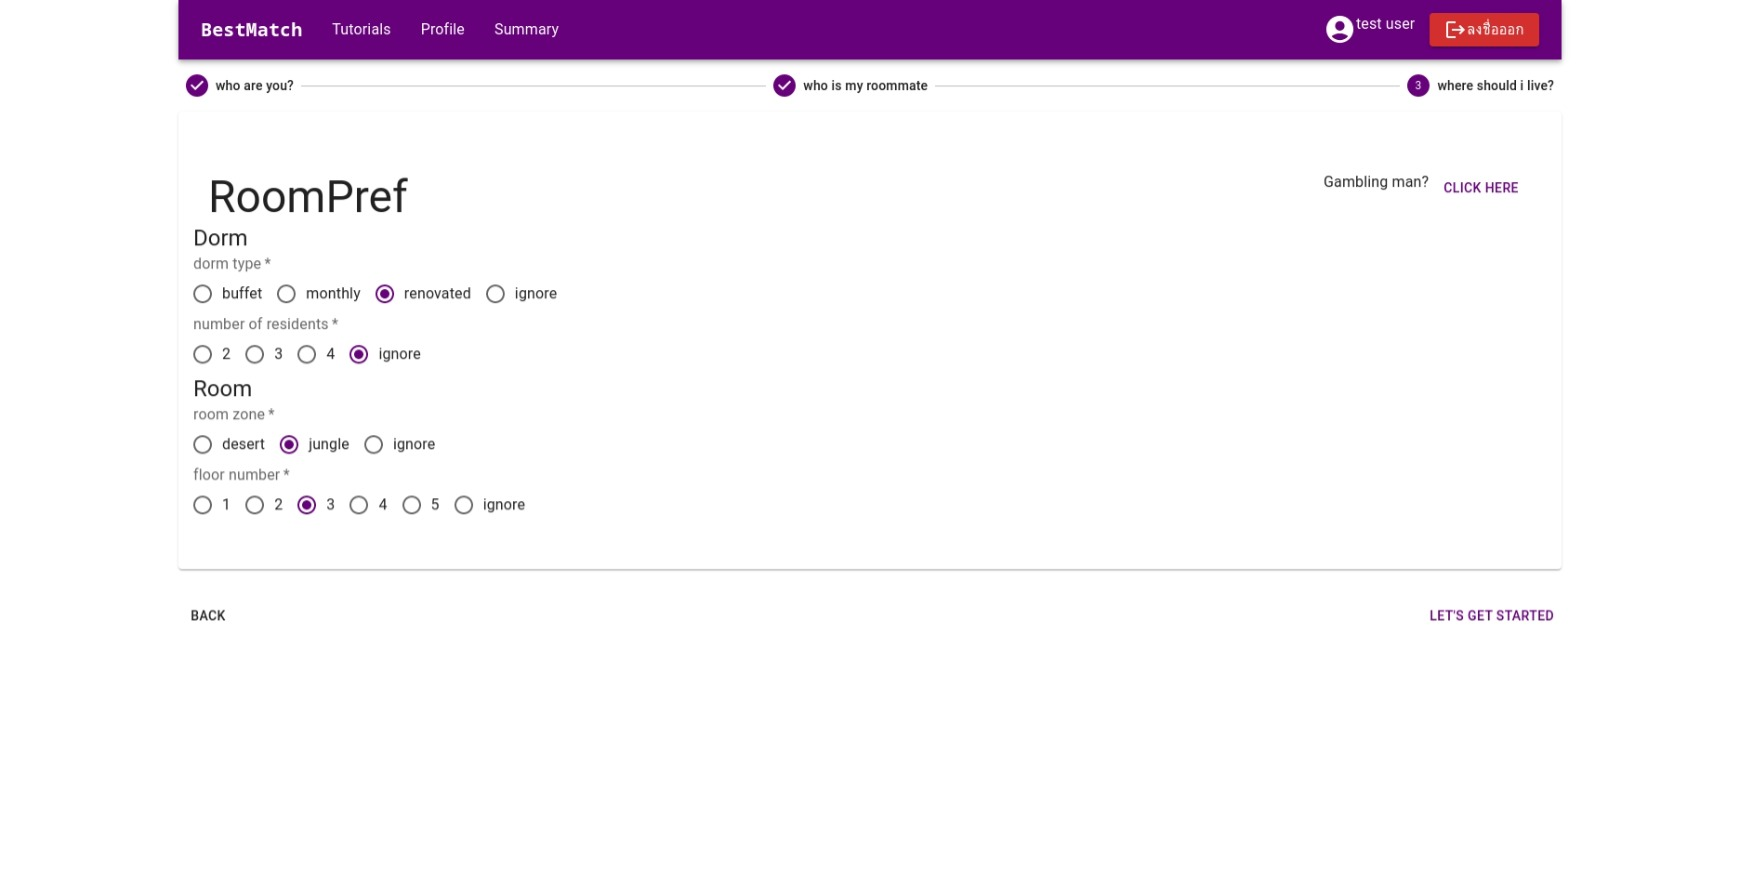
\includegraphics[width=\linewidth]{photo/web/student/dorm-def.jpeg}
          \end{center}
          \caption{หน้าระบุ $\mathit{roomPref}$ และ $\mathit{dormPref}$ ของนักศึกษา}
          \label{fig:room-pref}
        \end{figure}
        \clearpage
  \item นักศึกษาตรวจสอบคุณลักษณะของตนเอง และสามารถแก้ไขหากมีข้อผิดพลาดได้ด้วยปุ่ม edit
        \begin{figure}[ht]
          \begin{center}
            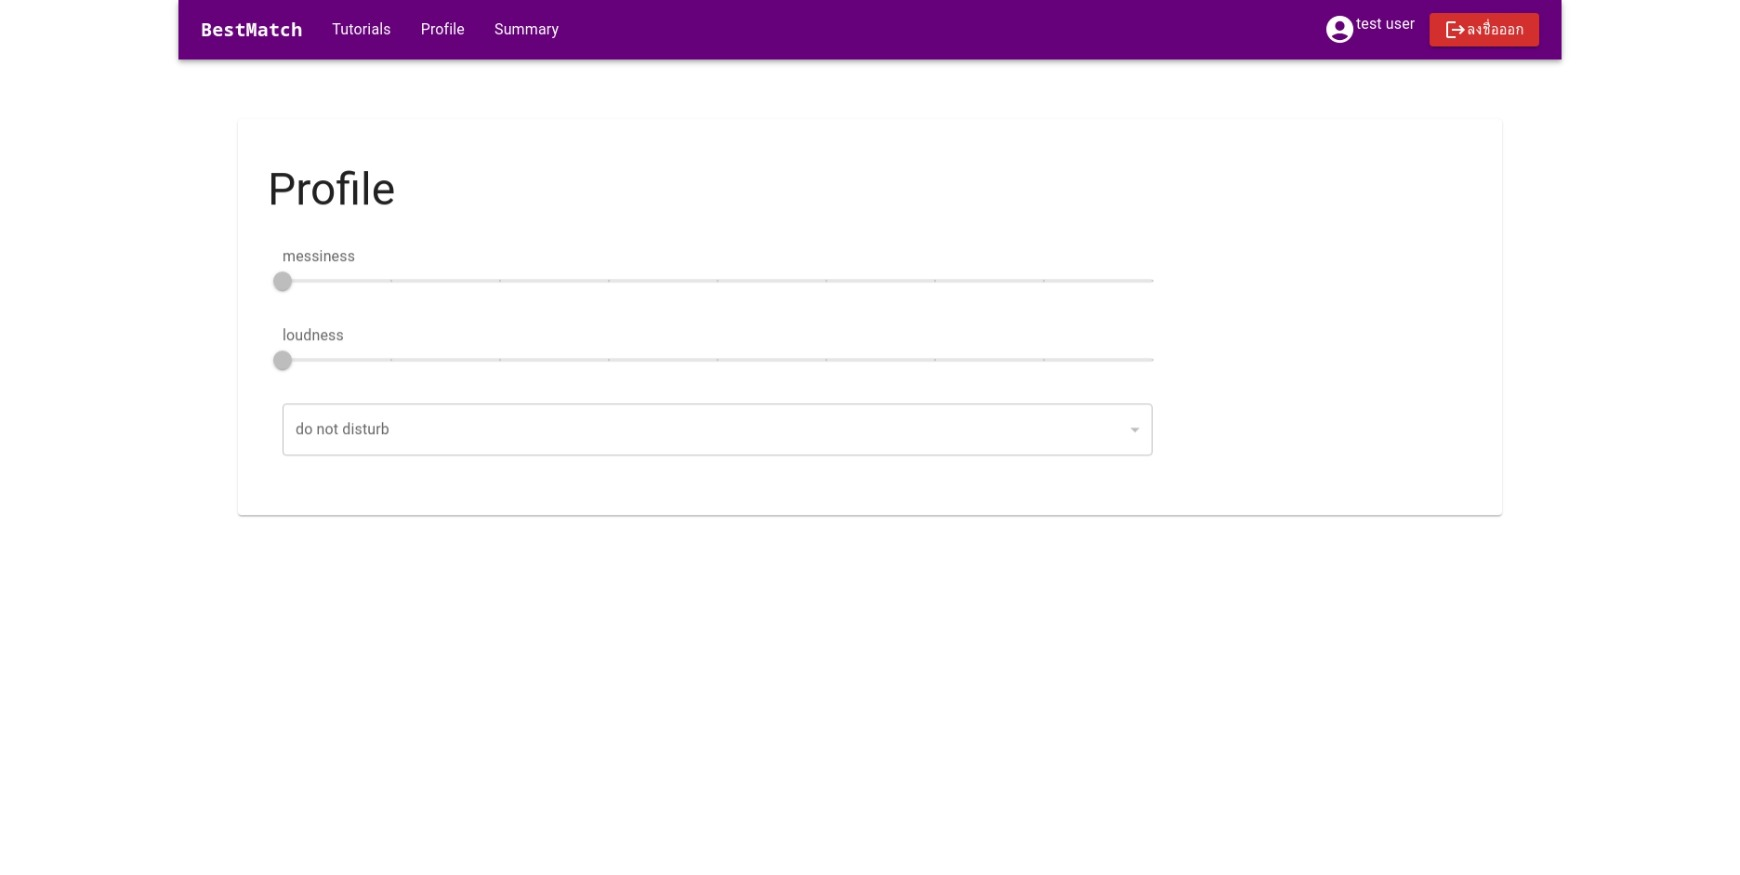
\includegraphics[width=\linewidth]{photo/web/student/profile.jpeg}
          \end{center}
          \caption{หน้าโปรไฟล์}
          \label{fig:profile}
        \end{figure}
        \clearpage
  \item นักศึกษาตรวจสอบคุณลักษณะของผู้ร่วมอาศัยที่คาดว่าจะได้รับหลังจากระบบสิ้นสุดการประมวลผล
        \begin{figure}[ht]
          \begin{center}
            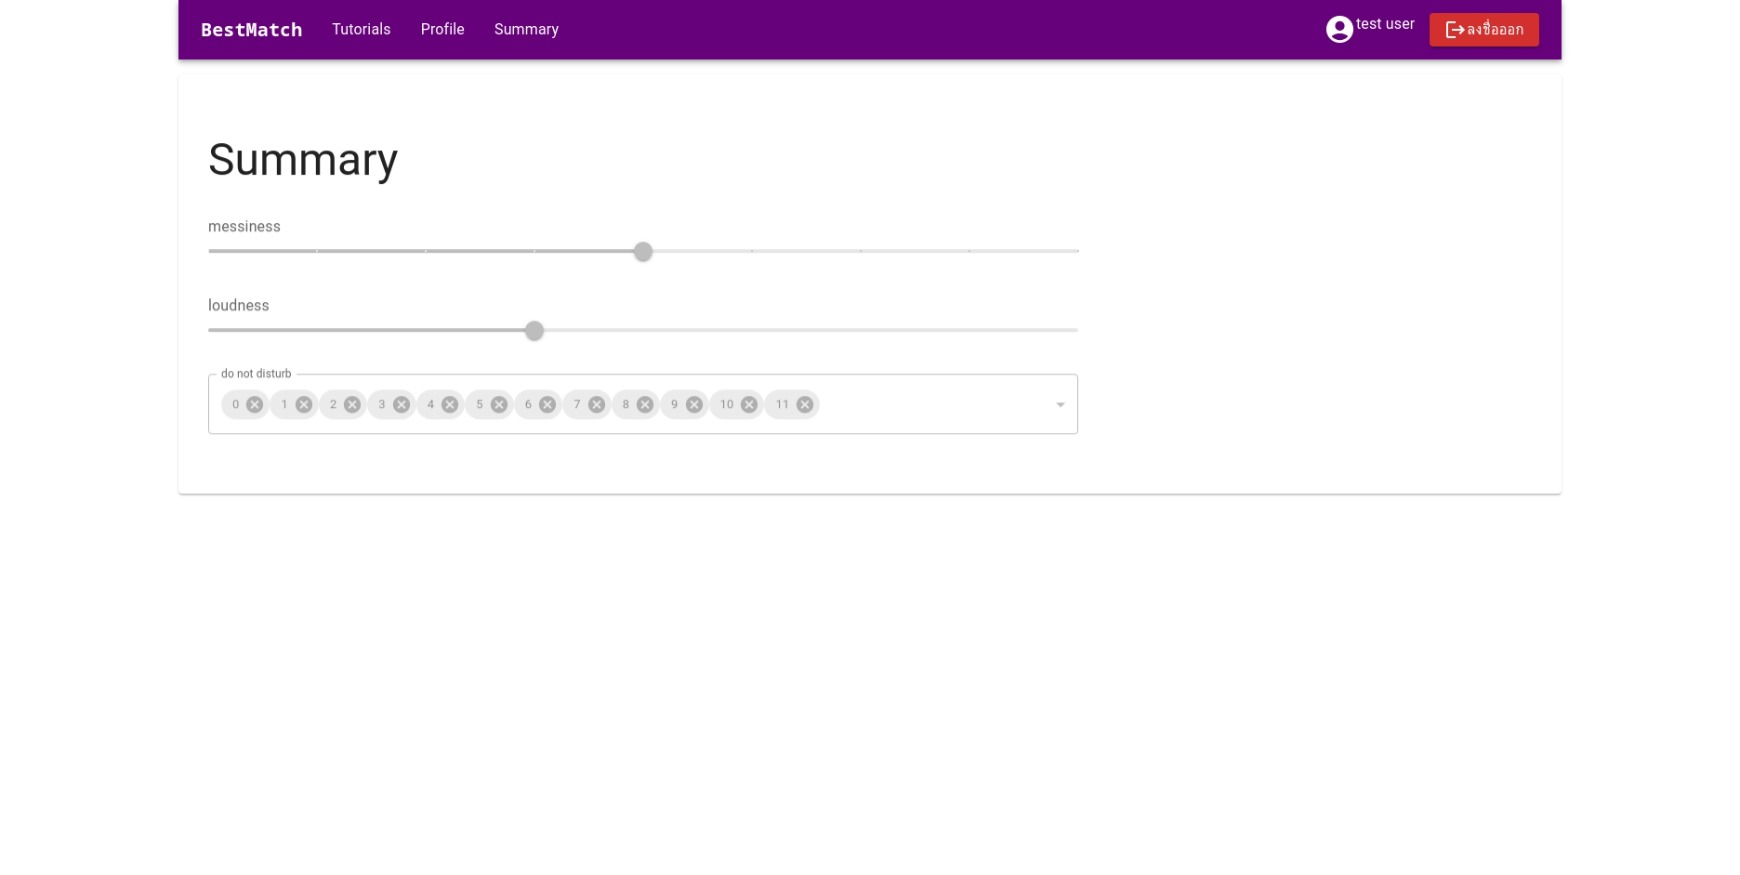
\includegraphics[width=\linewidth]{photo/web/student/summary.jpeg}
          \end{center}
          \caption{หน้าสรุปผลคุณลักษณะที่ผู้ใช้ให้ความสนใจ}
          \label{fig:summary}
        \end{figure}
        % \item ระบบยืนยันตัวตน: ให้ผูู้ใช้ลงทะเบียนสมัครสมาชิกและเข้าสู่ระบบเพื่อที่จะสามารถใช้งานระบบต่างๆของระบบได้ต่อไป
        % \item ระบบการจัดอันดับคุณลักษณะ: ให้ผู้ใช้ที่ลงชื่อเข้าใช้แล้วเลือกคุณสมบัติของห้องและเพื่อนร่วมห้องที่ต้องการ
        % \item ระบบปรับจูนคุณลักษณะ: ระบบจะทำการนำโปรไฟล์ของบุคคลอื่นๆ มาแสดงให้ผู้ใช้เลือกว่า หากเป็นบุคคลที่มี
        %       คุณลักษณะตามโปรไฟล์ ผู้ใช้จะเลือกบุคคลดังกล่าวเป็นเพื่อนร่วมห้องหรือไม่ เพื่อคำนวณหาระดับความใส่ใจในคุณลักษณะต่างๆของผู้ใช้ 
        %       ตัวอย่างดังรูปที่~\ref{fig:finetune}
        % \item ระบบรายงานสรุปผล: แสดงความคืบหน้าว่า ณ ปัจจุบันผู้ใช้มีโอกาสจะได้จับคู่กับเพื่อนร่วมห้องที่มีคุณลักษณะอย่างไร
        %       และจะได้ห้องแบบใด 
        % \item ระบบคู่มือการใช้งาน: แสดงคู่มือการใช้งานของระบบสำหรับผู้ใช้ทั่วไป ไม่รวมผู้ใช้ที่เป็นผู้ดูแลระบบ
        % \item ระบบโปรไฟล์ผู้ใช้: ให้ผู้ใช้เข้าไปปรับแต่งคุณลักษณะของตนเองเพื่อนำไปใช้ในการจับคู่กับผู้อื่น
\end{enumerate}

% \subsection{ผู้ดูแล}
% ส่วนของผู้ดูแลนั้นยังไม่มีการออกแบบ แต่เบื้องต้นคาดว่าจะเป็นแบบ dashboard 1 หน้าดังรูป\ME{...}{ใส่รูปตัวอย่าง dashboard} ที่สามารถบริหารจัดการสิ่งต่างๆ ต่อไปนี้
% \begin{enumerate}
%   \item ผู้ดูแลเพิ่มลด และแก้ไขข้อมูลของหอพัก เพื่อนำข้อมูลไปใช้ในการระบุห้องที่เปิดให้จองในระบบ
%   \item ผู้ดูแลระบุรายการห้องพักที่ไม่เปิดให้จอง โดยใช้รูปแบบ และประเภทไฟล์ที่ระบบกำหนดเบื้องต้นคาดว่าให้ผู้ดูแลระบุเป็นรายการในการจัดการห้อง
%   \item ผู้ดูแลตั้งค่าวันที่เปิด--ปิดระบบ โดยผู้ดูแลสามารถตั้งค่าได้ด้วยหน้าต่างใช้งาน หรืออาจใช้ไฟล์ที่ระบุห้องพักระบุวันเปิด--ปิดเช่นกัน
        % \item ระบบจัดการเวลาเปิด--ปิดวันลงทะเบียน: ให้ผู้ดูแลระบบสามารถตั้งค่าเวลาเปิด--ปิด
        % วันลงทะเบียนของผู้ใช้ทั่วไป
        % \item ระบบจัดการฐานข้อมูลและการตั้งค่าหอพักที่ใช้ในการลงทะเบียน: ให้ผู้ดูแลหอพักสามารถเลือกจัดการห้องและหอที่จะเปิดให้ลงทะเบียนในระบบได้
        % โดยการกดปุ่มเพิ่มเพื่อเพิ่มหอพัก กดปุ่มแก้ไขเพื่อแก้ไขจำนวนและเลขห้องที่เปิดให้ลงทะเบียนในระบบของหอนั้นๆ และกดปุ่มลบเพื่อลบหอนั้นๆออกจากระบบลงทะเบียน
        % \item ระบบศูนย์รวมไฟล์แม่แบบของระบบลงทะเบียน: ให้ผู้ดูแลระบบสามารถเข้ามาดาวน์โหลดไฟล์แม่แบบที่ต้องใช้ในการจัดการระบบฐานข้อมูล\CIreply{mention template}
        % ยกตัวอย่างเช่น ไฟล์แม่แบบการตั้งค่าห้องพักที่จะเปิดให้ลงทะเบียน ภายในไฟล์จะมีฟอร์มที่มีหัวข้อที่ต้องกรอกจัดเตรียมไว้ให้แล้ว ซึ่งไฟล์ทั้งหมดจะเป็นไฟล์สกุล .csv
        % \begin{figure}[h]
        % \begin{center}
        % 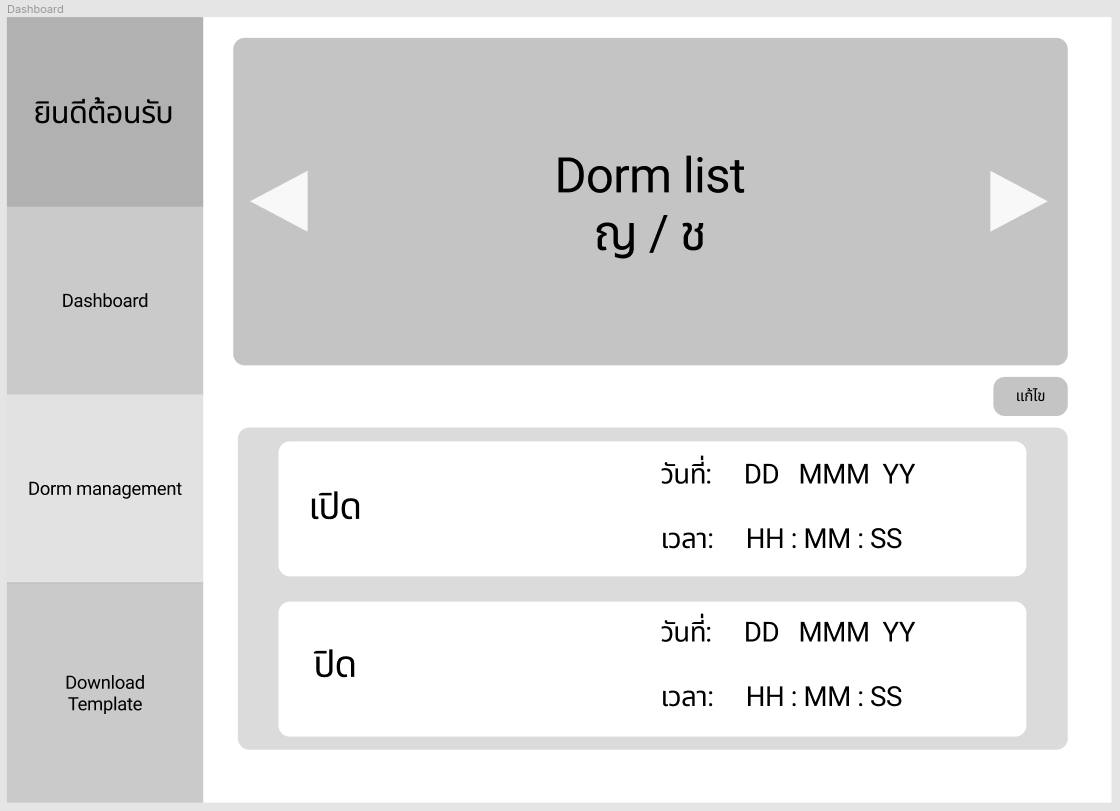
\includegraphics[width=\linewidth]{photo.old/adminDashboard.png}
        % \end{center}
        % \caption{หน้า homepage ของผู้ดูแลระบบ}
        % \label{fig:dashboard}
        % \end{figure}
        % \begin{figure}[h]
        % \begin{center}
        % 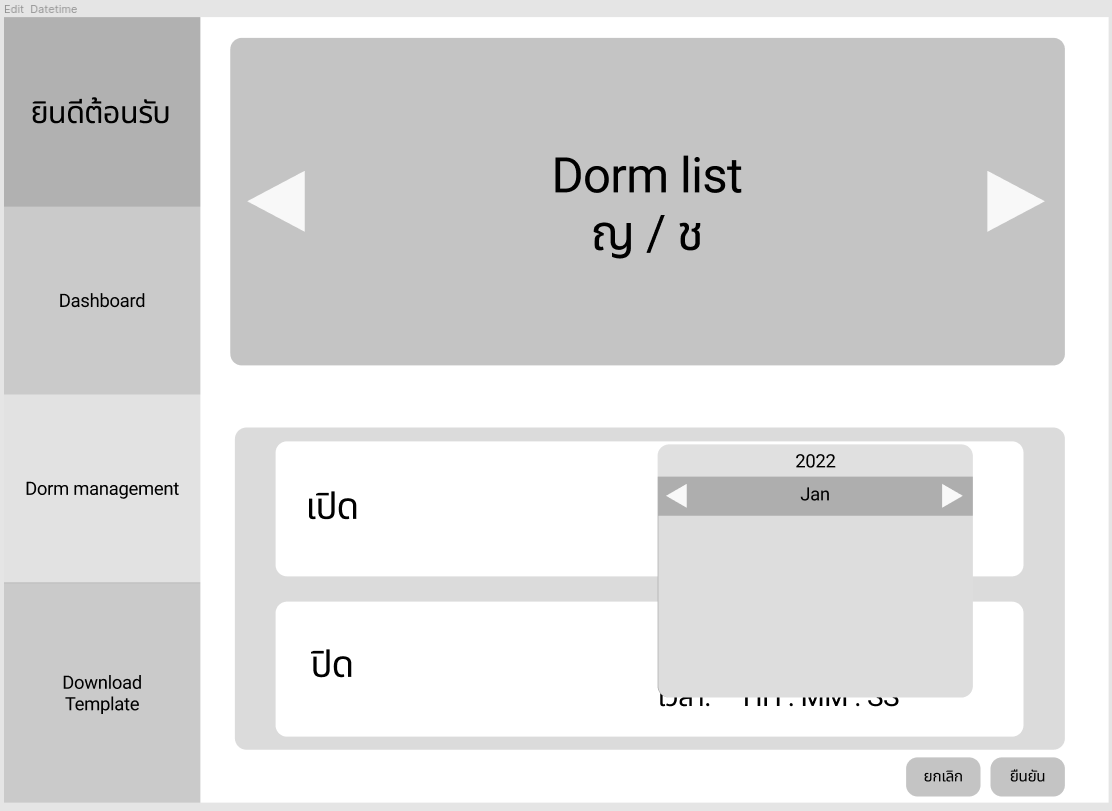
\includegraphics[width=\linewidth]{photo.old/datepicker.png}
        % \end{center}
        % \caption{ตัวอย่างการเปลี่ยนวันที่เปิด--ปิดระบบ}
        % \label{fig:datepicker}
        % \end{figure}
        % \begin{figure}[h]
        % \begin{center}
        % 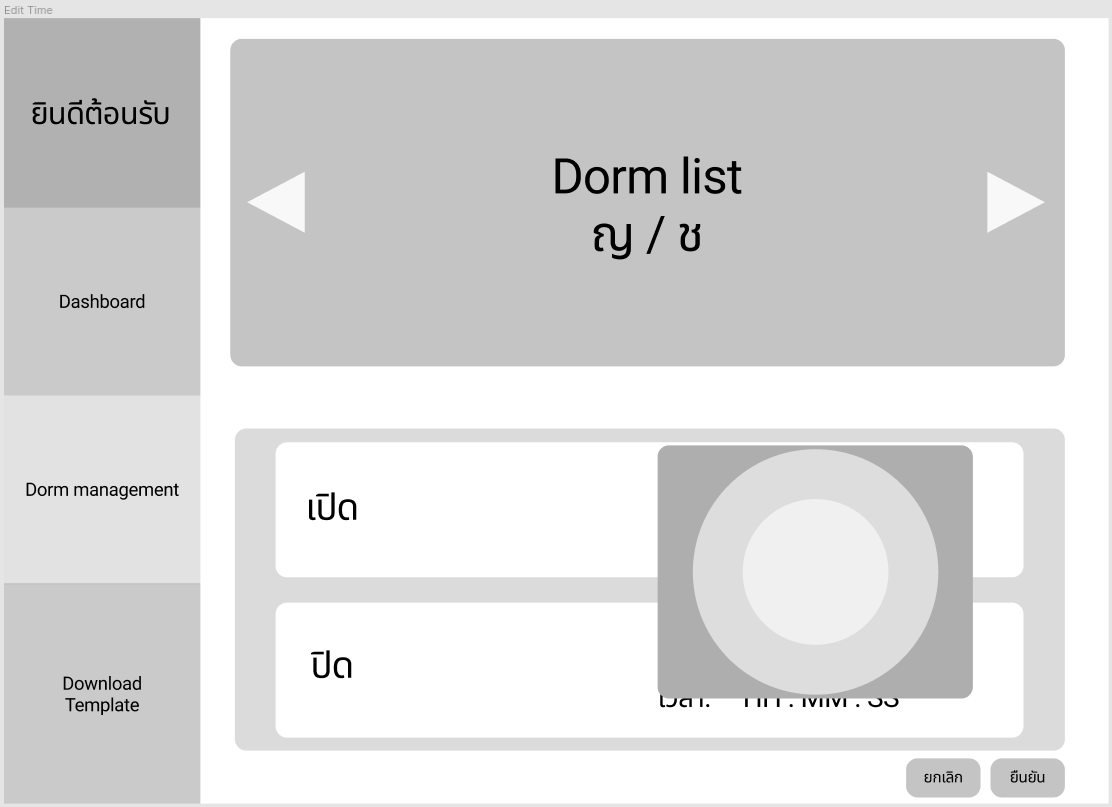
\includegraphics[width=\linewidth]{photo.old/timepicker.png}
        % \end{center}
        % \caption{ตัวอย่างการเปลี่ยนเวลาที่เปิด--ปิดระบบ}
        % \label{fig:timepicker}
        % \end{figure}
        % \begin{figure}[h]
        % \begin{center}
        % 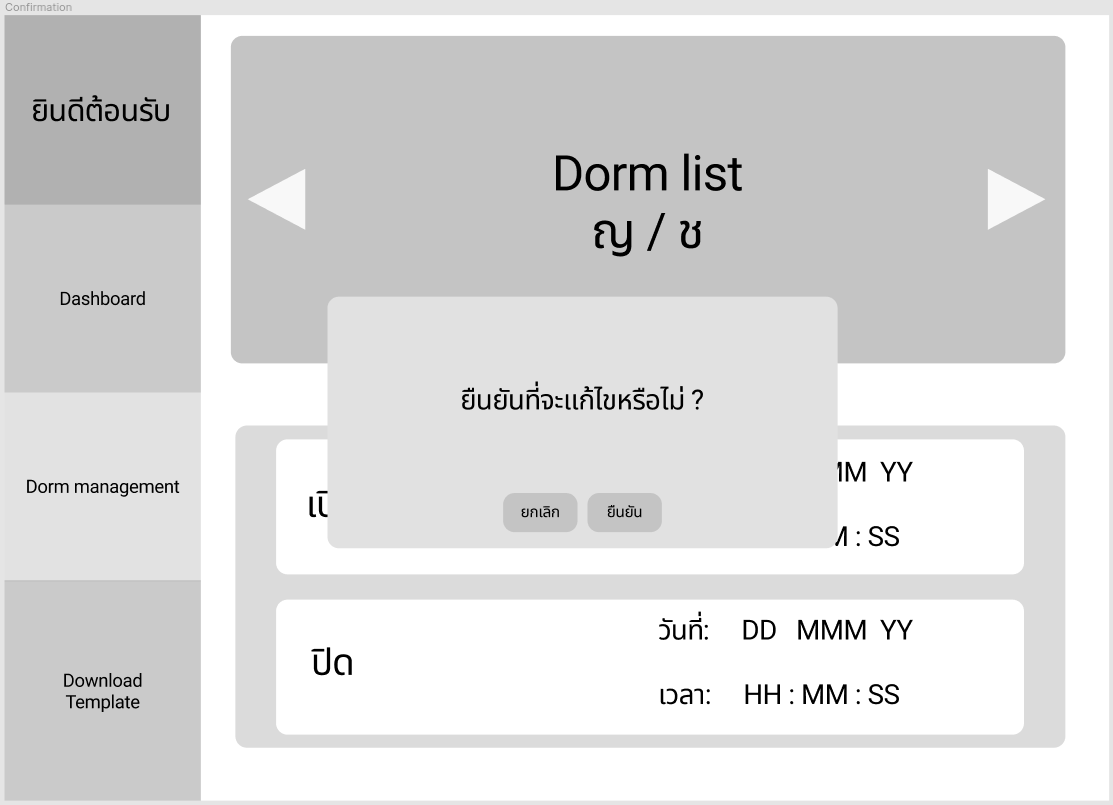
\includegraphics[width=\linewidth]{photo.old/confirmation.png}
        % \end{center}
        % \caption{ตัวอย่างแจ้งเตือนเพื่อยืนยันการตั้งค่า}
        % \label{fig:confirm-date-time}
        % \end{figure}
        
        % \clearpage
        % \begin{figure}[h]
        % \begin{center}
        % 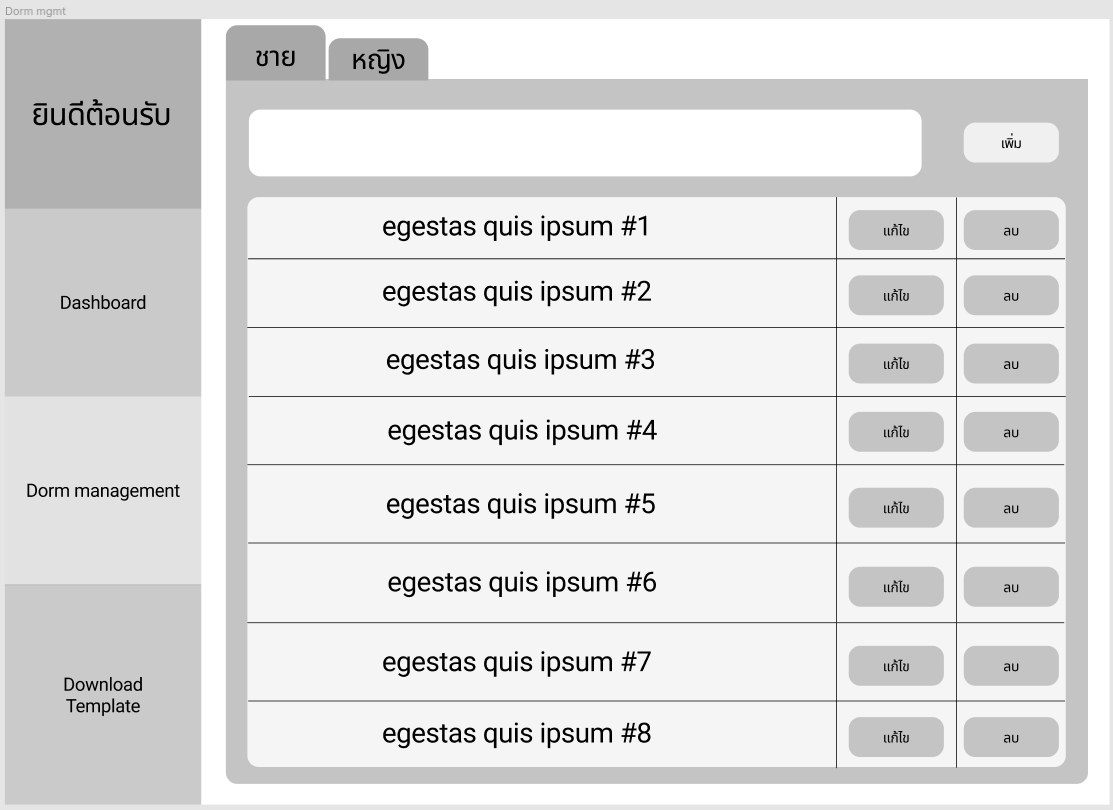
\includegraphics[width=\linewidth]{photo.old/dormmgmt.png}
        % \end{center}
        % \caption{หน้าการจัดการหอพักของระบบจอง}
        % \label{fig:mgmt}
        % \end{figure}
        % \begin{figure}[h]
        % \begin{center}
        % 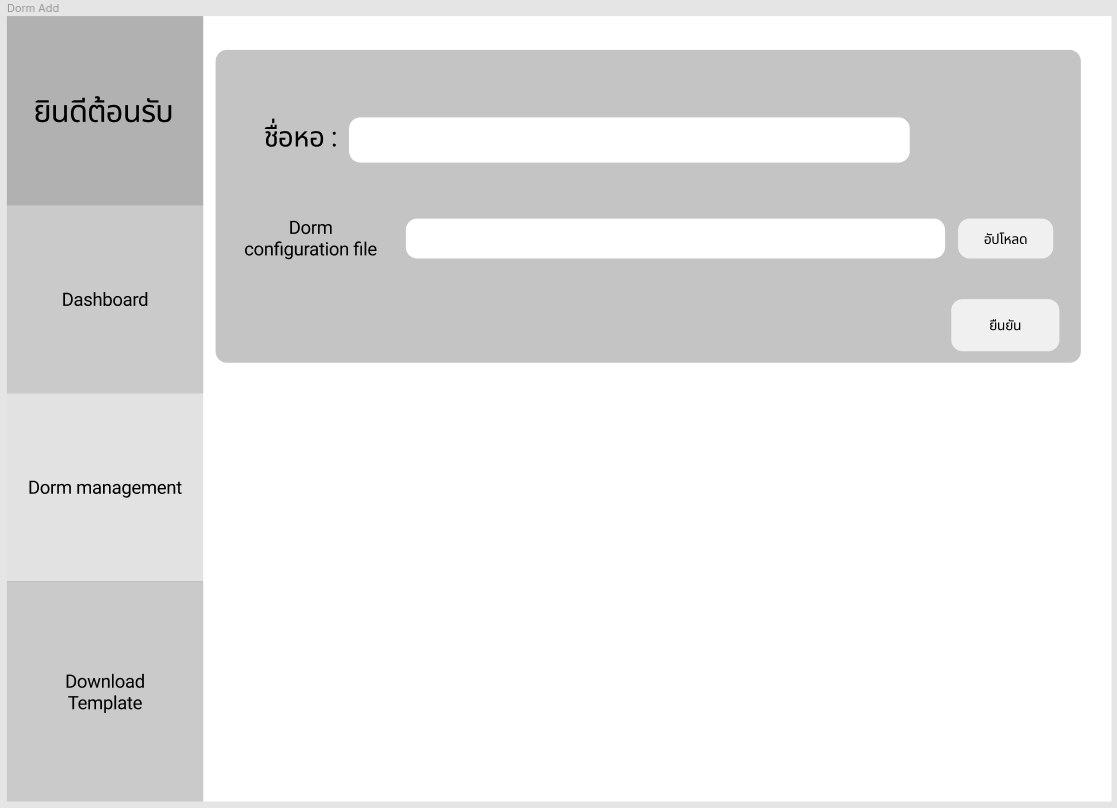
\includegraphics[width=\linewidth]{photo.old/dormadd.png}
        % \end{center}
        % \caption{หน้าการเพิ่มหอพักในระบบลงทะเบียน}
        % \label{fig:add-dorm}
        % \end{figure}
        % \begin{figure}[h]
        %   \begin{center}
        %   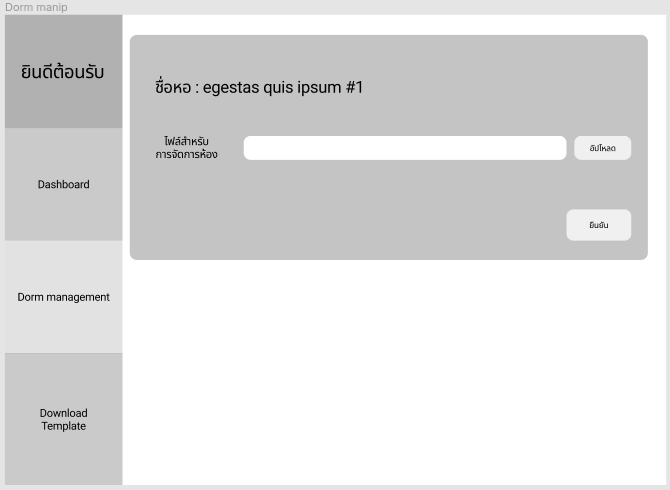
\includegraphics[width=\linewidth]{photo.old/roommgmt.png}
        %   \end{center}
        %   \caption{หน้าการจัดการเพิ่มลดห้องที่เปิดในระบบลงทะเบียน}
        %   \label{fig:room-mgmt}
        %   \end{figure}
        
        % \clearpage
        % \CIreply{ดาวน์โหลดไฟล์พวกนี้ไปเพื่ออะไร?}
        % \begin{figure}[h]
        % \begin{center}
        % 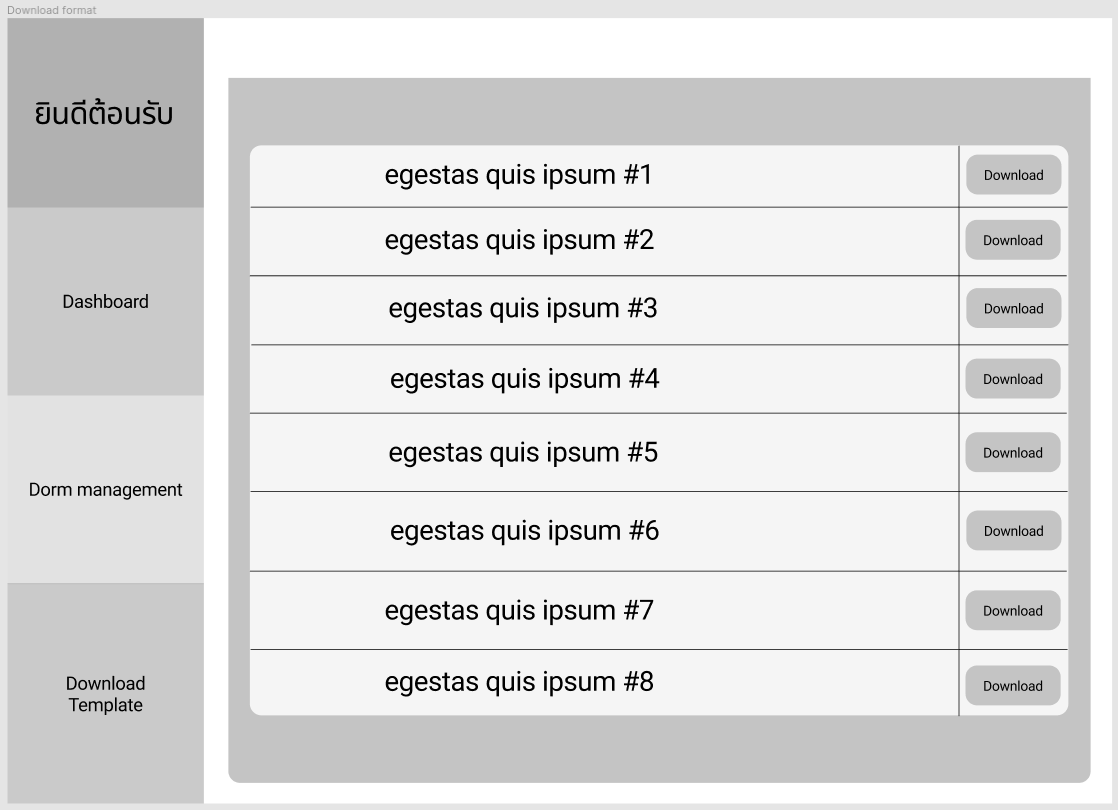
\includegraphics[width=\linewidth]{photo.old/format.png}
        % \end{center}
        % \caption{หน้าดาวน์โหลดไฟล์}
        % \label{fig:format-db}
        % \end{figure}
% \end{enumerate}

\chapter{\ifproject%
\ifenglish Experimentation and Results\else การทดลองและผลลัพธ์\fi
\else%
\ifenglish System Evaluation\else การประเมินระบบ\fi
\fi}

ในบทนี้จะทดสอบเกี่ยวกับการทำงานในฟังก์ชันหลักๆ

\section{วิธีการตรวจสอบความถูกต้องของระบบ}
\subsection{End-user}
\begin{enumerate}
    \item ระบบยืนยันตัวตน: ทดสอบว่าผู้ใช้สามารถลงทะเบียน ยืนยันตัวตน และสามารถปิดกั้นการเข้าถึงส่วนของระบบที่ต้องผ่านการลงทะเบียนก่อนได้ถูกต้อง
    \item ระบบการจัดอันดับคุณลักษณะ: คุณลักษณะที่ถูกจัดอันดับถูกแปรเปลี่ยนเป็นตัวเลขที่นำไปใช้ในอัลกอริทึมมีการแปลงที่ถูกต้อง
    \item ระบบปรับจูนคุณลักษณะ: มีการปรับปรุงตัวเลขที่\CI{สะท้อนถึง}{จะวัดอย่างไร}คุณลักษณะที่ผู้ใช้ให้ความสมใจในโปรไฟล์ที่เลือกมา
    \item ระบบรายงานสรุปผล: สรุปผลที่ได้จากการจัดอันดับ และการปรับจูนได้ถูกต้องตามความเป็นจริง
    \item ระบบคู่มือการใช้งาน: แสดงผลคู่มือการใช้งานที่มีลำดับขั้นตอนถูกต้องครบถ้วนสมบูรณ์
    \item ระบบโปรไฟล์ผู้ใช้: มีการจัดเก็บถูกต้อง ตรงกับที่ผู้ใช้งานกรอกเข้าสู่ระบบ
\end{enumerate}

\subsection{Administrator}
\begin{enumerate}
    \item ระบบจัดการเวลาเปิด--ปิดวันลงทะเบียน: ระบบเปิด--ปิดวันลงทะเบียนได้ถูกต้องตามที่ตั้งค่าไว้
    \item ระบบจัดการฐานข้อมูลและการตั้งค่าหอพักที่ใช้ในการลงทะเบียน: การตั้งค่าของหอและห้องพักที่เปิดให้ลงทะเบียนมีความถูกต้องตรงกับไฟล์ตั้งค่า
    \item ระบบจัดการไฟล์ที่ใช้ในการจัดการระบบลงทะเบียน: เมื่อผู้ใช้ดาวน์โหลดไฟล์จะได้รับไฟล์ที่ต้องการได้ถูกต้อง
\end{enumerate}

% \section{ประสิทธิภาพของอัลกอริทึม}
\CIreply{load test?}

\ifproject
\chapter{\ifenglish Conclusions and Discussions\else บทสรุปและข้อเสนอแนะ\fi}

\section{\ifenglish Conclusions\else สรุปผล\fi}

นศ. ควรสรุปถึงข้อจำกัดของระบบในด้านต่างๆ ที่ระบบมีในเนื้อหาส่วนนี้ด้วย

\section{\ifenglish Challenges\else ปัญหาที่พบและแนวทางการแก้ไข\fi}

ในการทำโครงงานนี้ พบว่าเกิดปัญหาหลักๆ ดังนี้
\begin{enumerate}
  \item การจับคู่นั้นจริงๆ แล้วมีอัลกอริทึมที่ต้องคิด และพัฒนาทั้งหมด 3 ส่วน ซึ่งต้องใช้ข้อมูลจำนวนมากประกอบการพัฒนา
        ซึ่งทำให้ภาระงานเพิ่มขึ้นมากจากที่คาดการณ์เอาไว้ทำให้ไม่เหลือเวลาในการพัฒนาฟีเจอร์ส่วนอื่นๆ เช่น หน้าโปรไฟล์ หรือหน้าคู่มือการใช้งานที่ออกแบบไว้เป็นคู่มือที่ผู้ใช้จะสามารถปฏิสัมพันธ์ด้วยได้
  \item tRPC เป็นไลบรารีที่ค่อนข้างใหม่ ซึ่งทำให้การทดสอบและ การแก้ปัญหาดำเนินไปด้วยความยากลำบาก
\end{enumerate}


\section{\ifenglish%
Suggestions and further improvements
\else%
ข้อเสนอแนะและแนวทางการพัฒนาต่อ
\fi
}
% \begin{enumerate}
%   \item การจัดการ
% \end{enumerate}
เนื่องจากโครงการนี้ประกอบด้วยหลายฟีเจอร์ที่ใหญ่ ซึ่งจะทำให้มีงานย่อยๆที่ต้องทำในแต่ละขั้นตอนเยอะจนอาจจะติดตามความคืบหน้าได้ลำบาก
จึงอยากแนะนำให้ลองใช้ซอฟต์แวร์จัดการโปรเจคเช่น Jira, Notion หรือ Trello

เนื่องจากเครื่องมือทดสอบ API เช่น Postman นั้นยังไม่รองรับกับ tRPC จึงอยากแนะนำให้ใช้ tRPC เป็นเพียงเหมือนสะพานเชื่อมระหว่าง Front-end
และ Back-end เท่านั้น ให้พัฒนา Back-end ด้วยไลบรารีหรือเฟรมเวิร์คเช่น Express หรือ NestJS เพื่อให้ง่ายต่อการทดสอบ

ในส่วนของการจับคู่นั้น วิธีการที่ออกแบบไว้ยังเป็นการไล่จับคู่ทีละคู่ๆ ซึ่งอาจจะหาวิธีการที่จะสามารถช่วยให้สามารถลดเวลาในการประมวลผลลงได้ 
จะทำให้แอพพลิเคชันนี้เหมาะสมกับการนำไปใช้งานมากยิ่งขึ้น เช่นการแบ่งกลุ่มของผู้ใช้ในการเลือกจับกลุ่ม อาจจะเป็นอัลกอริทึมที่มีลักษณะคล้ายๆกับการหา 
K-Nearest-Neigbour

เพิ่มส่วนการทำงานของฝั่งผู้ดูแล เช่น การตั้งค่าเวลาเปิด-ปิดระบบ การจัดการห้องที่สามารถ

\fi

\bibliography{report}

\ifproject
\appendix
% \chapter{The first appendix}

% Text for the first appendix goes here.

% \section{Appendix section}

% Text for a section in the first appendix goes here.

% test ทดสอบฟอนต์ serif

% \textsf{test ทดสอบฟอนต์ sans serif}

\ifenglish\else
% TODO: Thai teletype font still doesn't work with english option
% \verb+test ทดสอบฟอนต์ teletype ภาษาไทย+

% \texttt{test ทดสอบฟอนต์ teletype ภาษาไทย}
\fi

\chapter{\ifenglish Manual\else คู่มือการใช้งานระบบ\fi}

%
เมื่อนักศึกษาเข้ามาที่เว็บแอพพลิเคชันจะพบกับหน้า Home
\begin{figure}[h]
  \begin{center}
    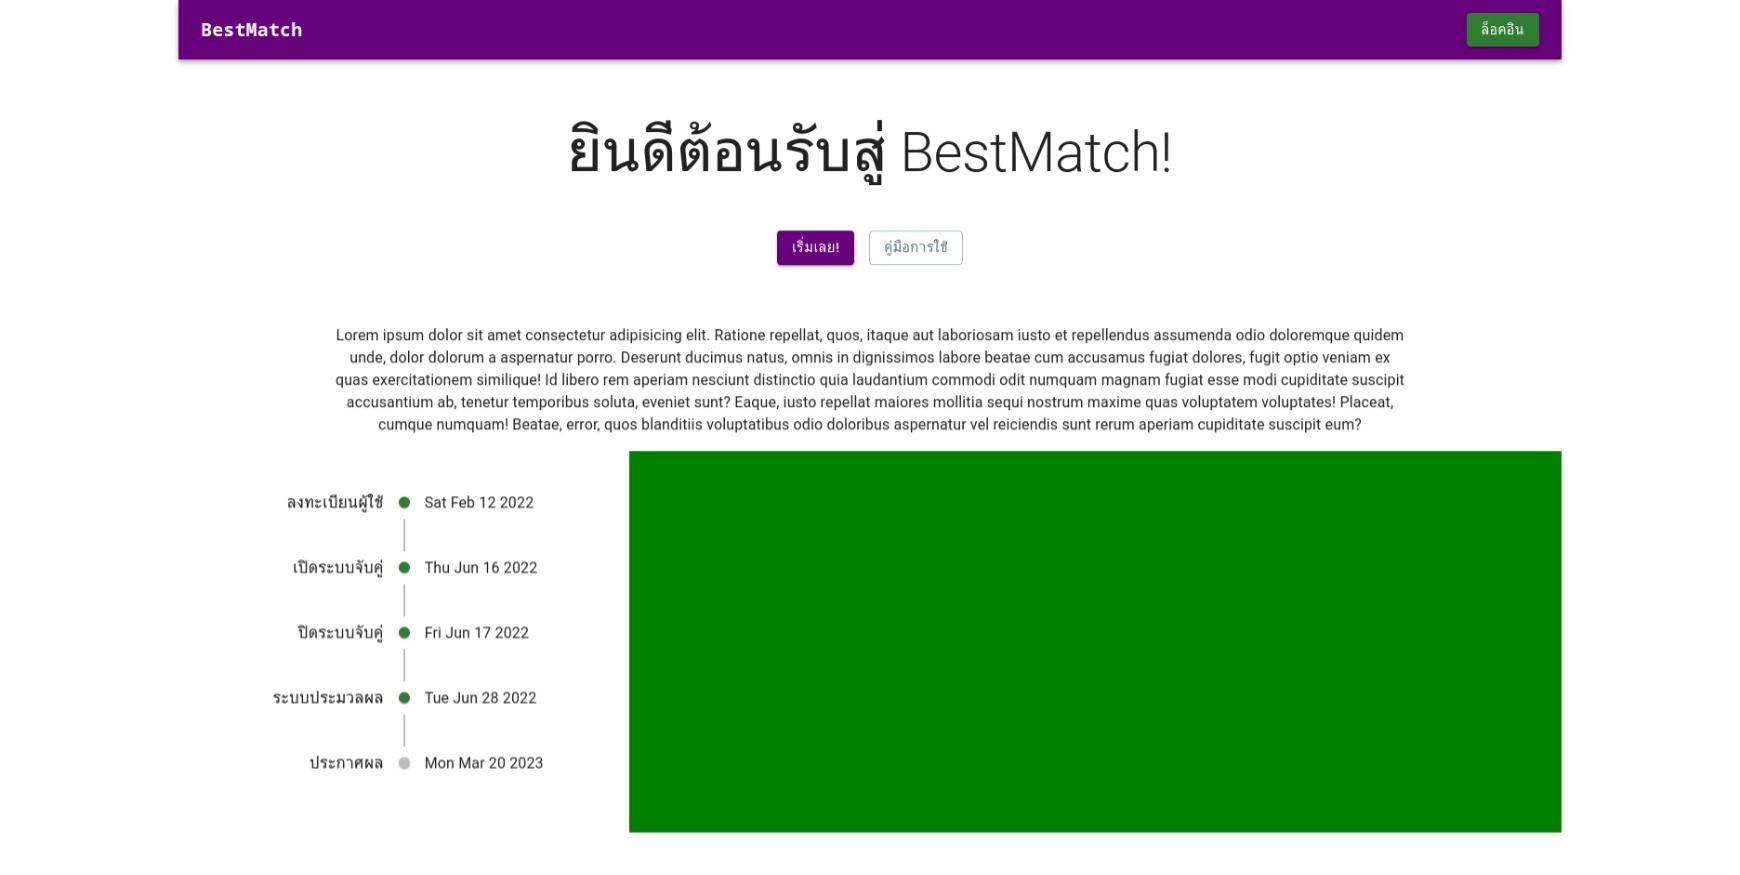
\includegraphics[width=\linewidth]{photo/web/student/home.jpeg}
  \end{center}
  \caption{หน้า Home}
\end{figure}
%
\newline
หลังจากนั้นจะกดปุ่ม "ล็อคอิน" หรือ "เริ่มเลย!" เพื่อทำการลงชื่อเข้าใช้
\begin{figure}[ht]
  \begin{center}
    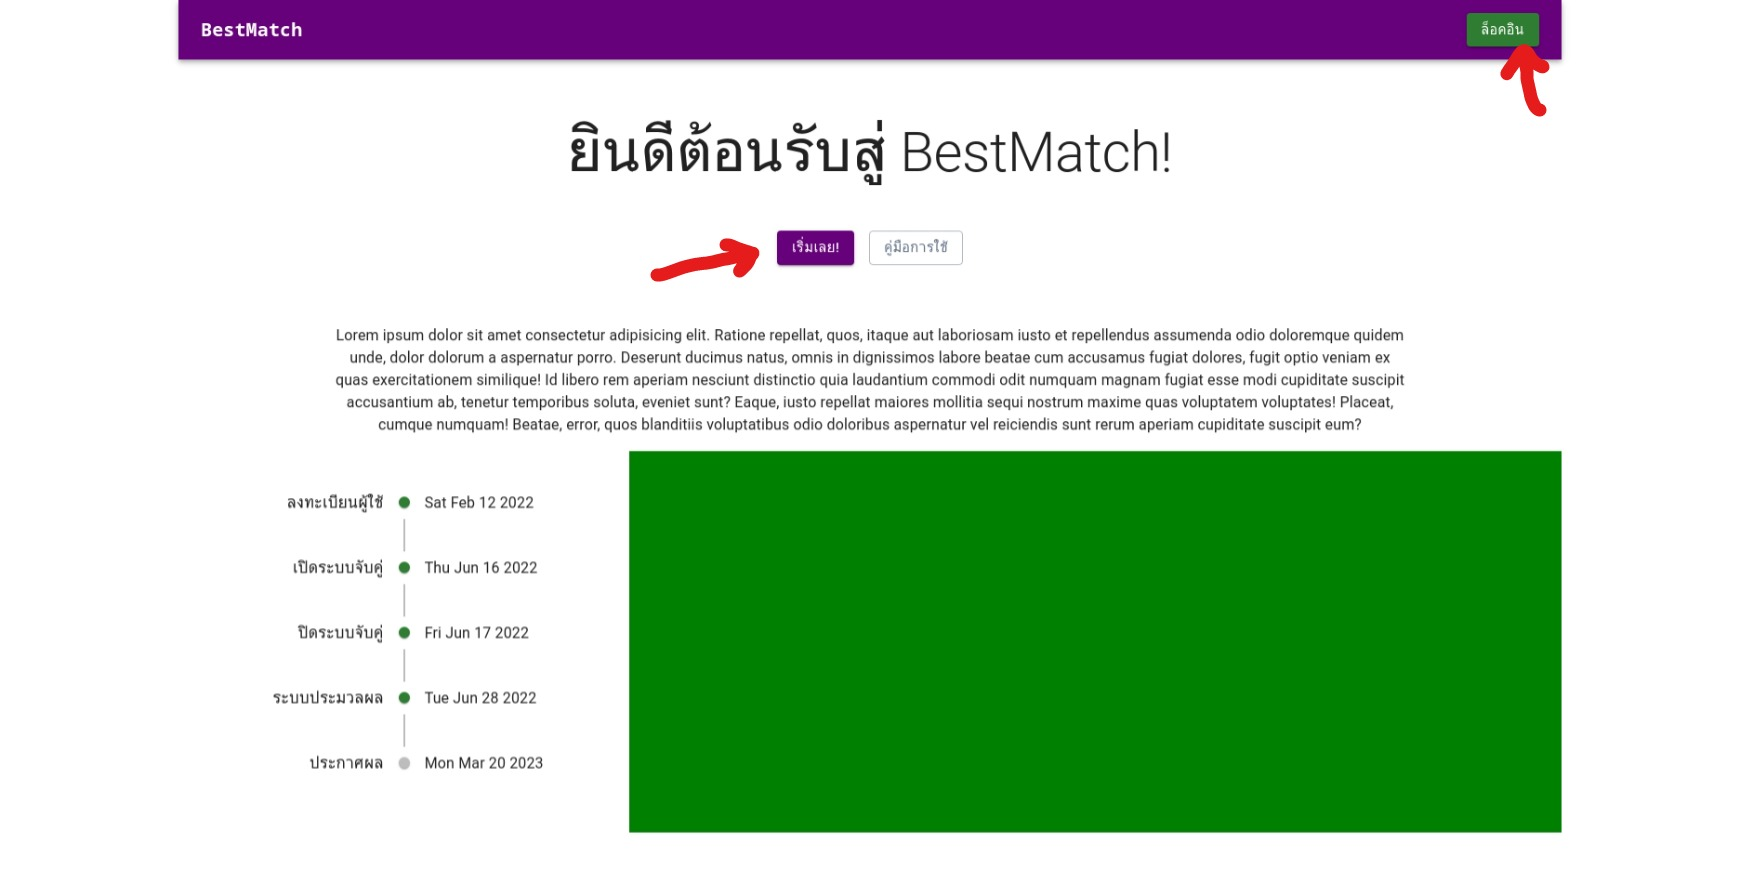
\includegraphics[width=\linewidth]{photo/web/student/login-btn.jpeg}
  \end{center}
  \caption{รูปตัวอย่างแสดงตำแหน่งปุ่ม "ล็อคอิน" และ "เริ่มเลย!"}
\end{figure}
\newpage 

หลังจากนั้นกรอกข้อมูลที่ใช้ในการยืนยันตัวตนในการเข้าใช้งาน
\begin{figure}[!ht]
  \begin{center}
    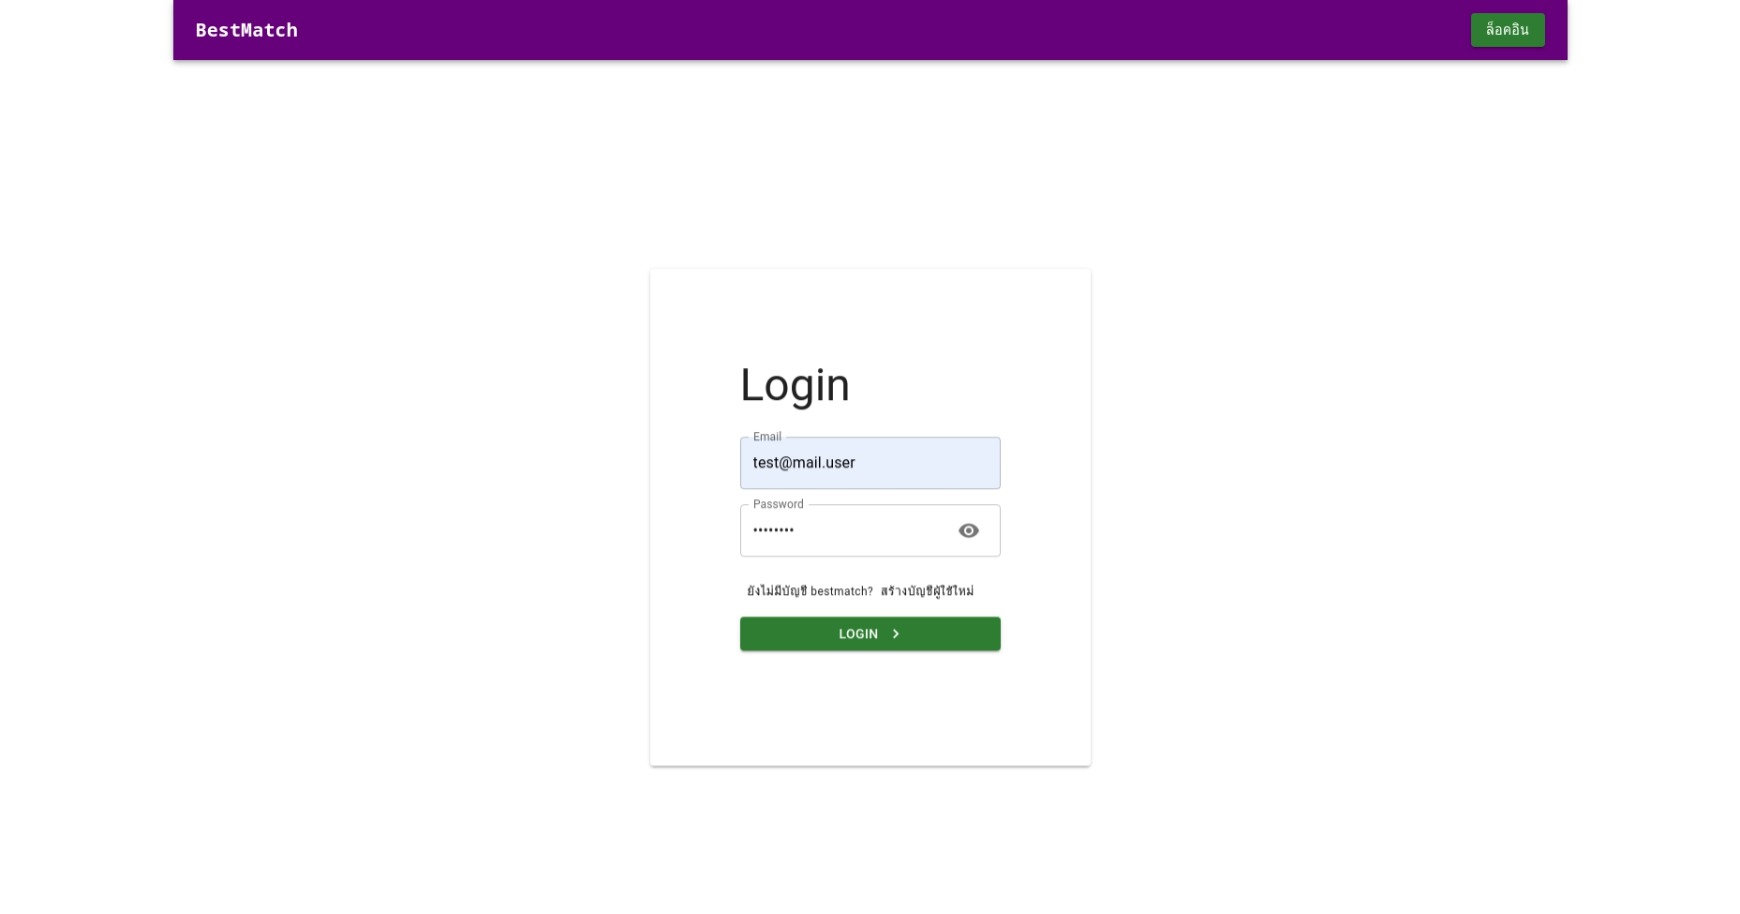
\includegraphics[width=\linewidth]{photo/web/student/login.jpeg}
  \end{center}
  \caption{หน้า Login}
\end{figure}
%
\newline
หากยังไม่มีบัญชีผู้ใช้จะต้องทำการสร้างบัญชีผู้ใช้โดยคลิกที่ "สร้างบัญชีผู้ใช้ใหม่"
\begin{figure}[!ht]
  \begin{center}
    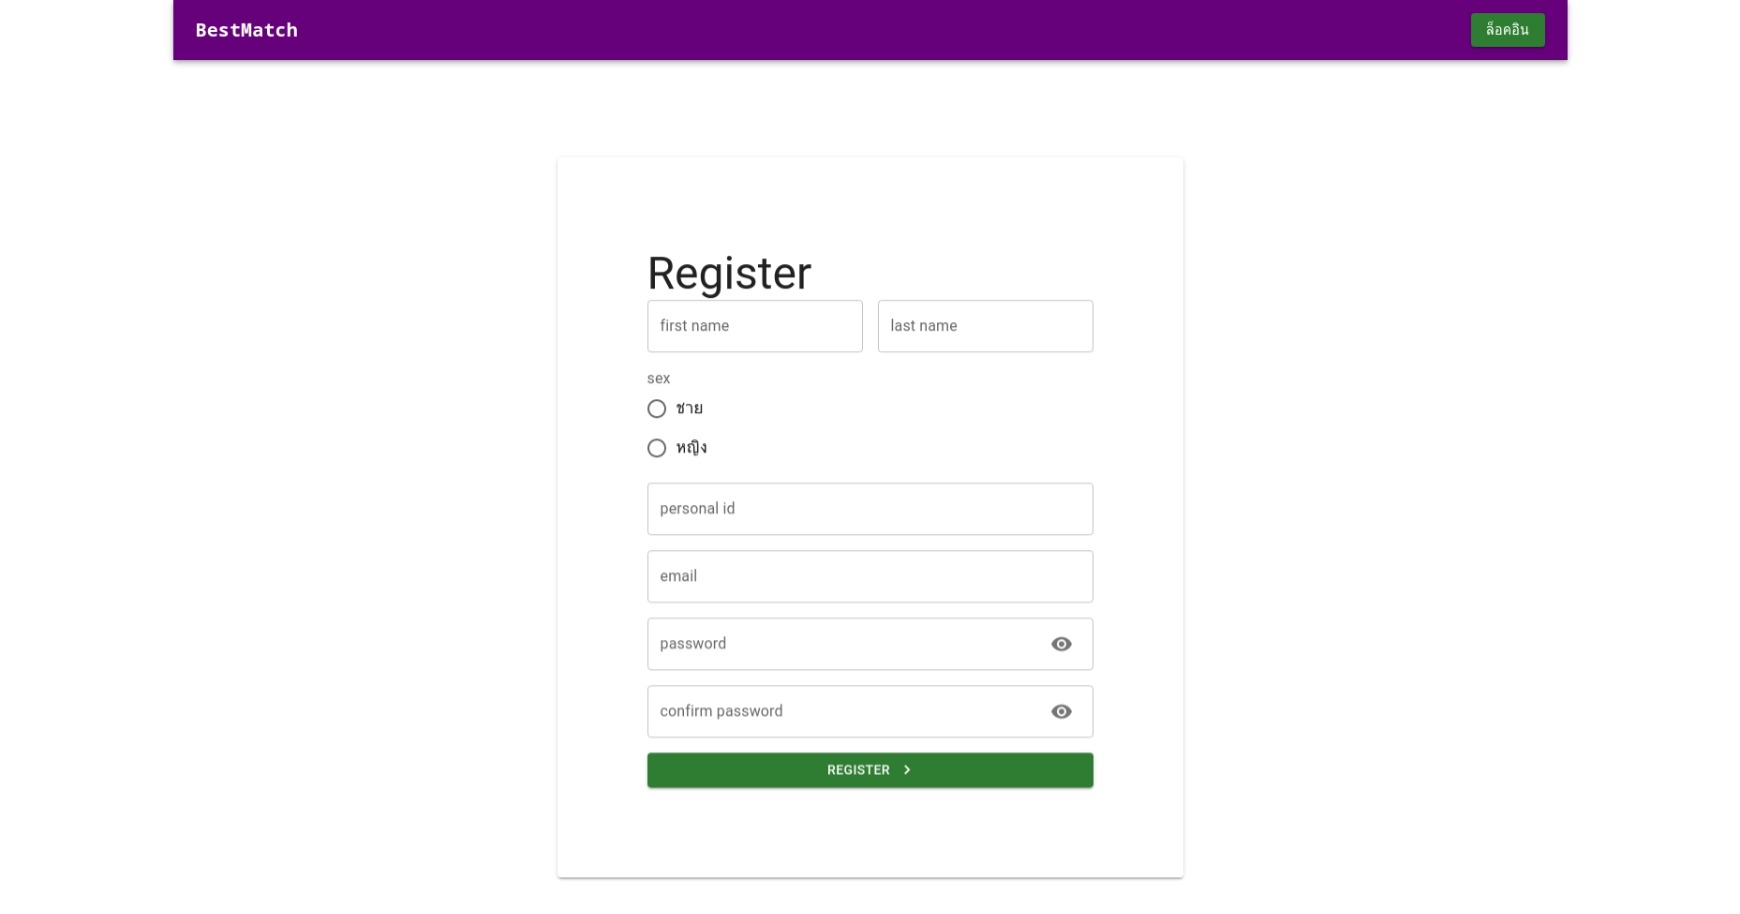
\includegraphics[width=\linewidth]{photo/web/student/register.jpeg}
  \end{center}
  \caption{หน้า Register}
\end{figure}
\newpage

เมื่อลงชื่อเข้าใช้แล้วจะกลับมาที่หน้า Home พร้อมกับอีเมล์ของผู้ใช้
\begin{figure}[!ht]
  \begin{center}
    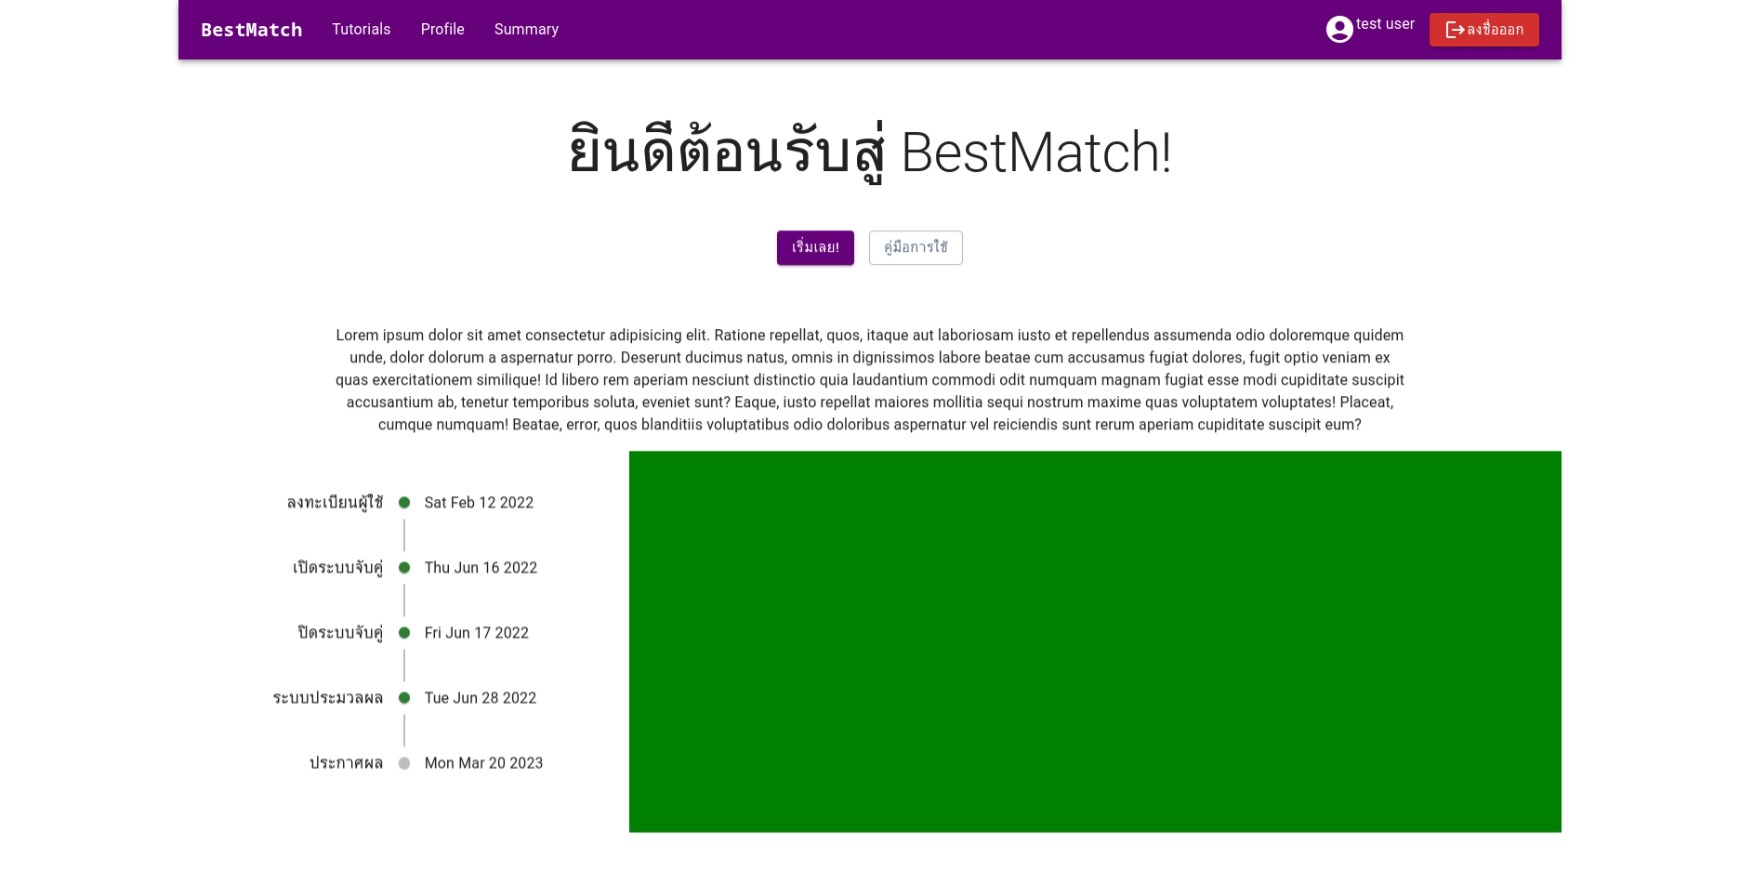
\includegraphics[width=\linewidth]{photo/web/student/home-auth.jpeg}
  \end{center}
  \caption{หน้า Home หลังยืนยันตัวตนสำเร็จ}
\end{figure}
%
\newline
เมื่อกดปุ่ม "เริ่มเลย" จะไปที่หน้าแอพพลิเคชันหลัก ซึ่งจะให้ผู้ใช้ระบุโปรไฟล์ของตนเอง
เสร็จแล้วกดปุ่ม "NEXT"
\begin{figure}[h]
  \begin{center}
    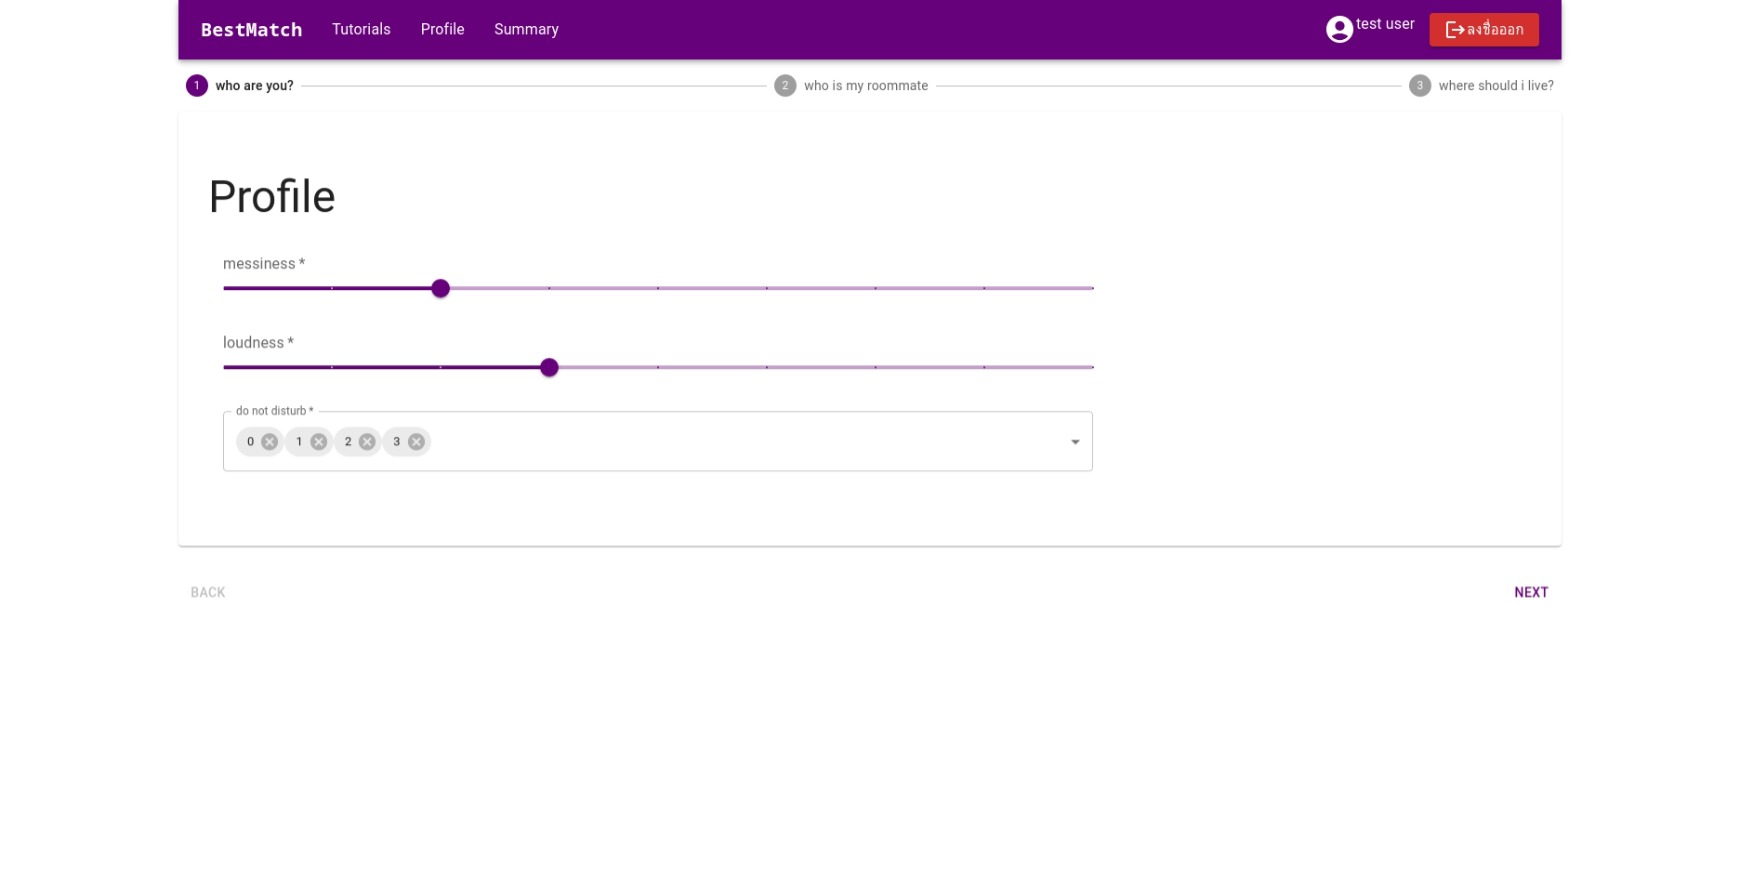
\includegraphics[width=\linewidth]{photo/web/student/profile-def.jpeg}
  \end{center}
  \caption{หน้าระบุ profile ของผู้ใช้}
\end{figure}
\newpage

หลังจากนั้นระบุ preference ของรูมเมทที่ต้องการ เมื่อเสร็จแล้วกดปุ่ม "NEXT"
\begin{figure}[h]
  \begin{center}
    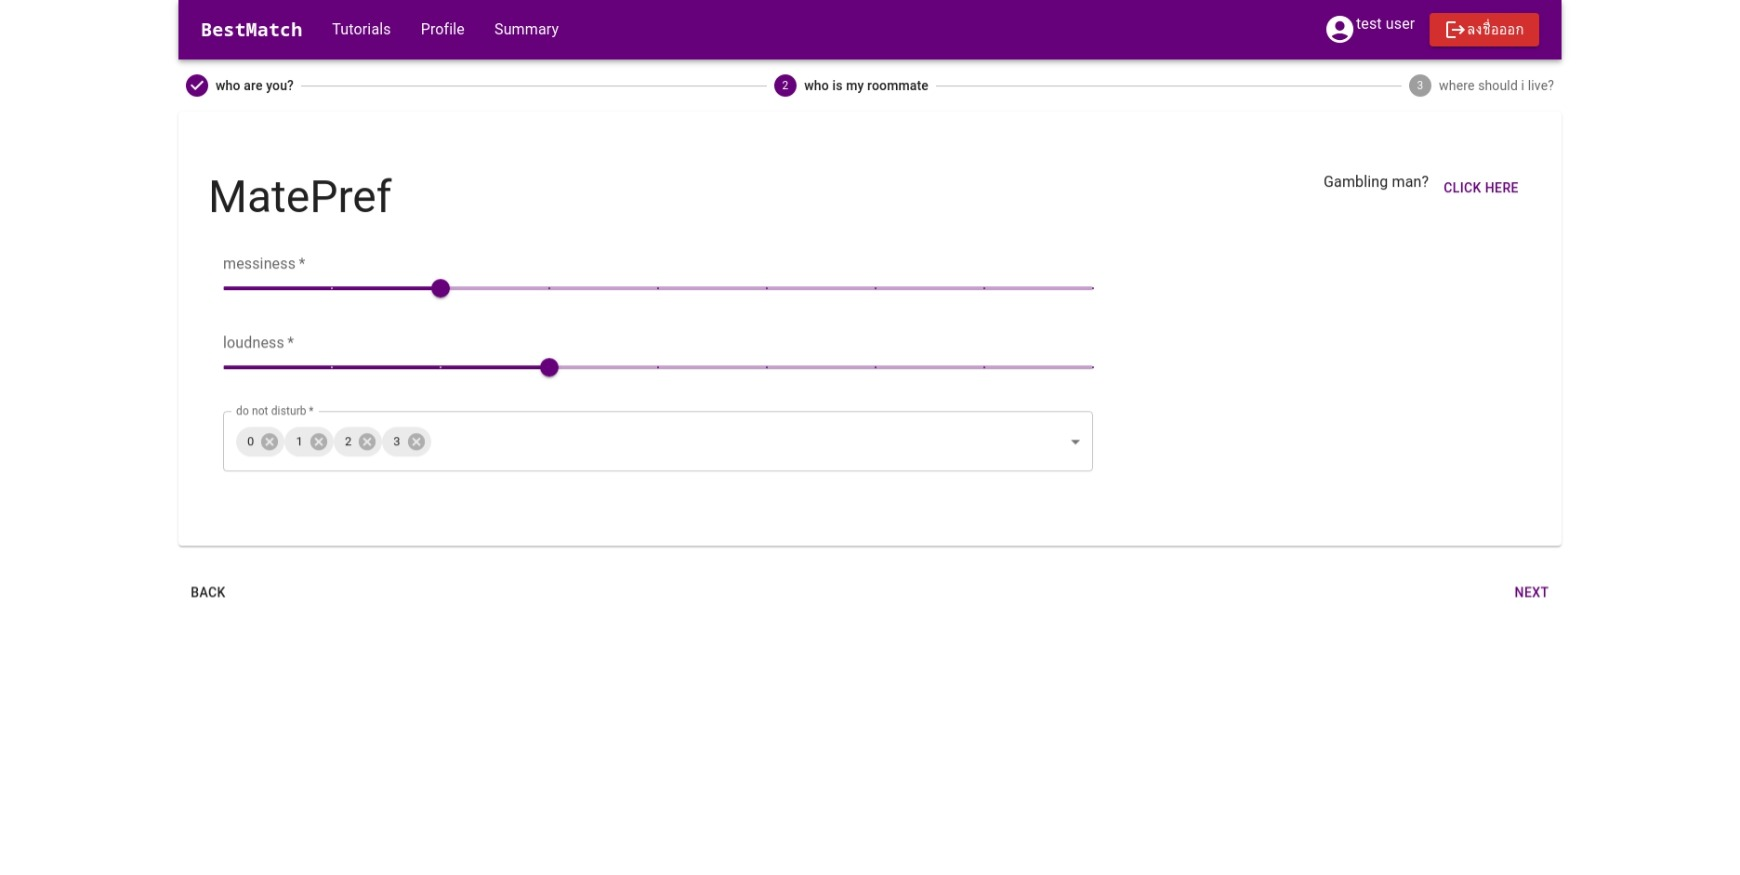
\includegraphics[width=\linewidth]{photo/web/student/mate-def.jpeg}
  \end{center}
  \caption{หน้า preference ของรูมเมท}
\end{figure}
%
\newline
โดยหากผู้ใช้ไม่อยากระบุ preference ของรูมเมทก็สามารถกด "CLICK HERE" ได้
\begin{figure}[h]
  \begin{center}
    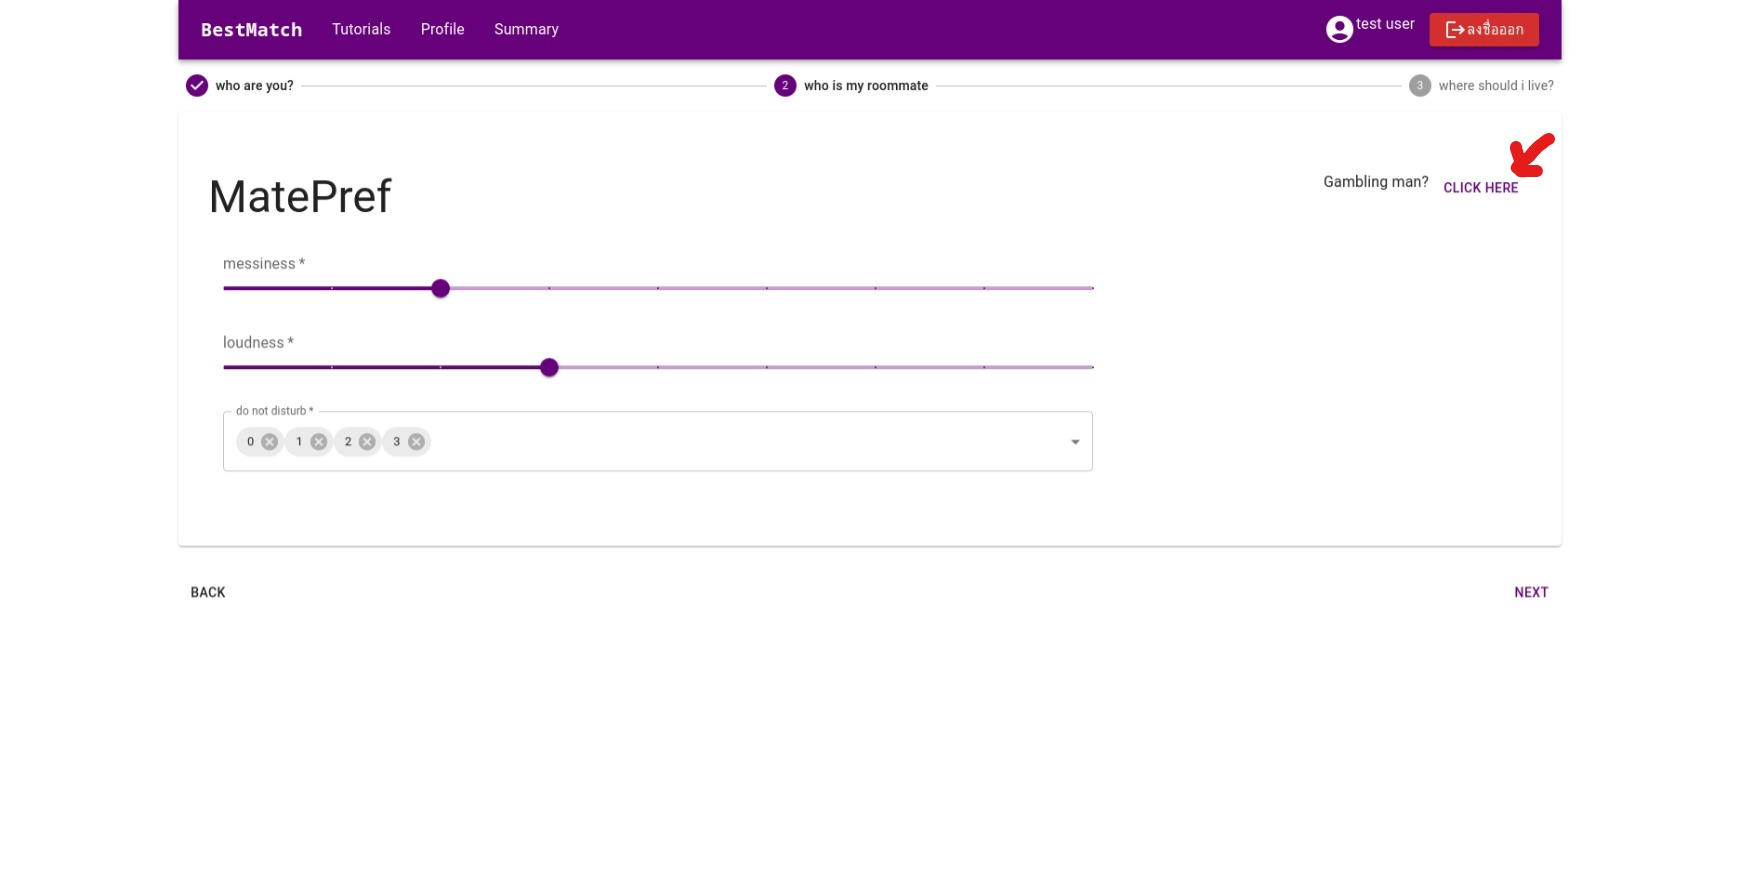
\includegraphics[width=\linewidth]{photo/web/student/mate-gambler.jpeg}
  \end{center}
  \caption{รูปตัวอย่างแสดงตำแหน่งปุ่ม "CLICK HERE" ของหน้า preference ของรูมเมท}
\end{figure}
\newpage

หลังจากนั้นระบุ preference ของห้อง และ หอพักที่ต้องการ เมื่อเสร็จแล้วกดปุ่ม "NEXT"
\begin{figure}[h]
  \begin{center}
    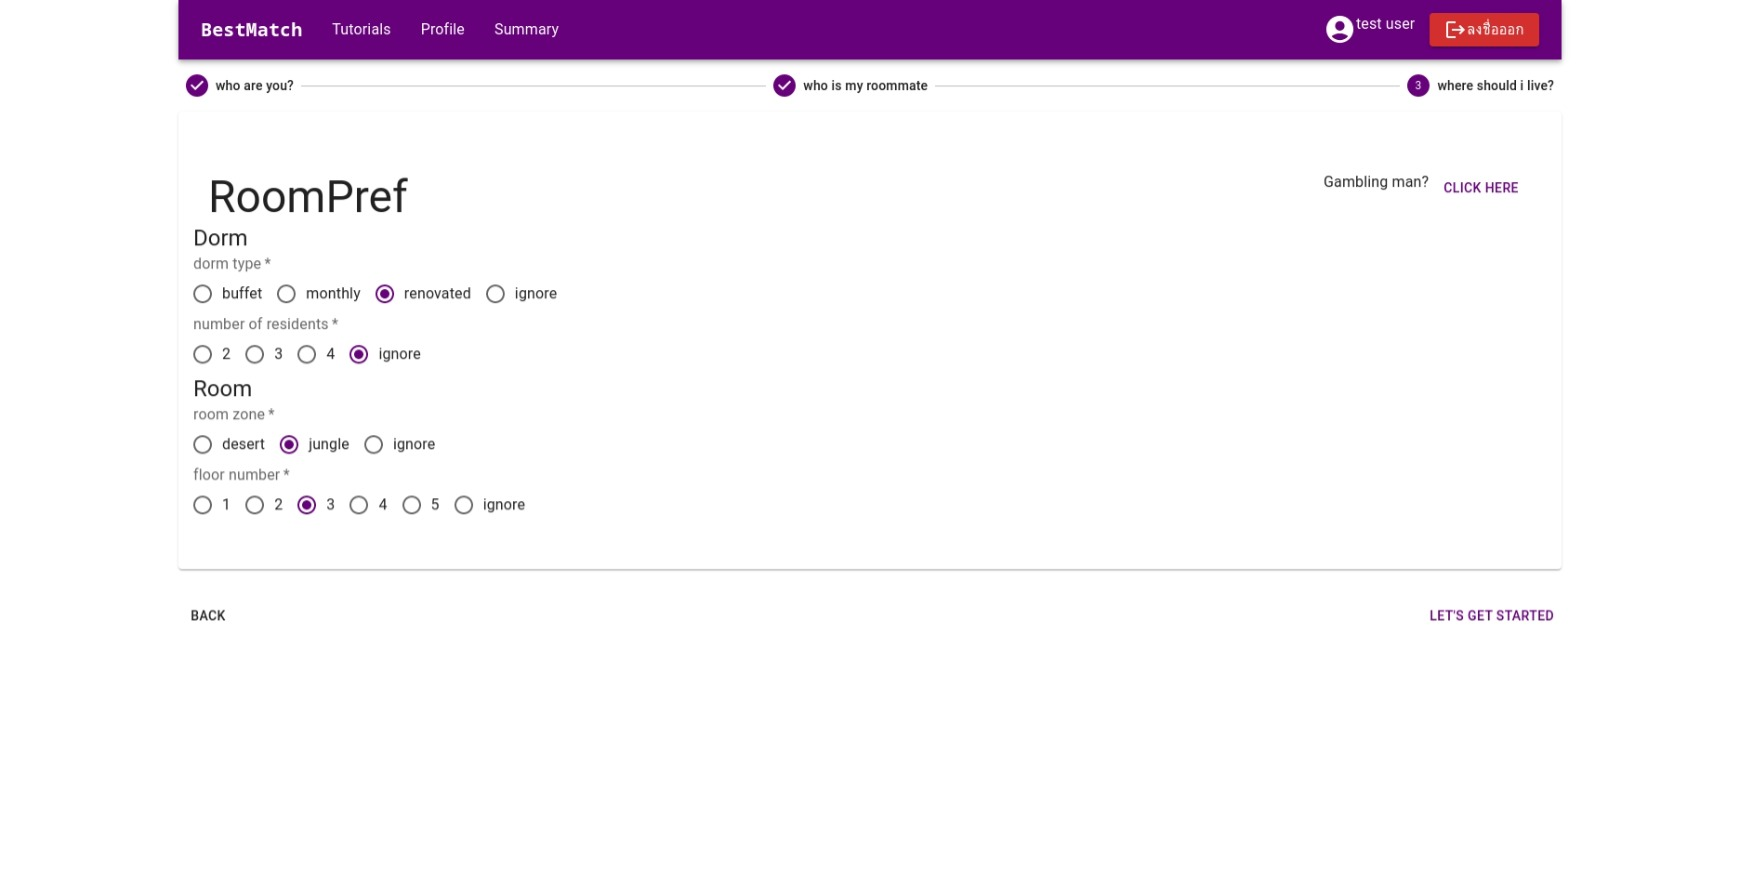
\includegraphics[width=\linewidth]{photo/web/student/dorm-def.jpeg}
  \end{center}
  \caption{หน้า preference ของหอพัก}
\end{figure}
%
\newline
โดยหากผู้ใช้ไม่อยากระบุ preference ของหอพัก และห้องพักก็สามารถกด "CLICK HERE" ได้
\begin{figure}[h]
  \begin{center}
    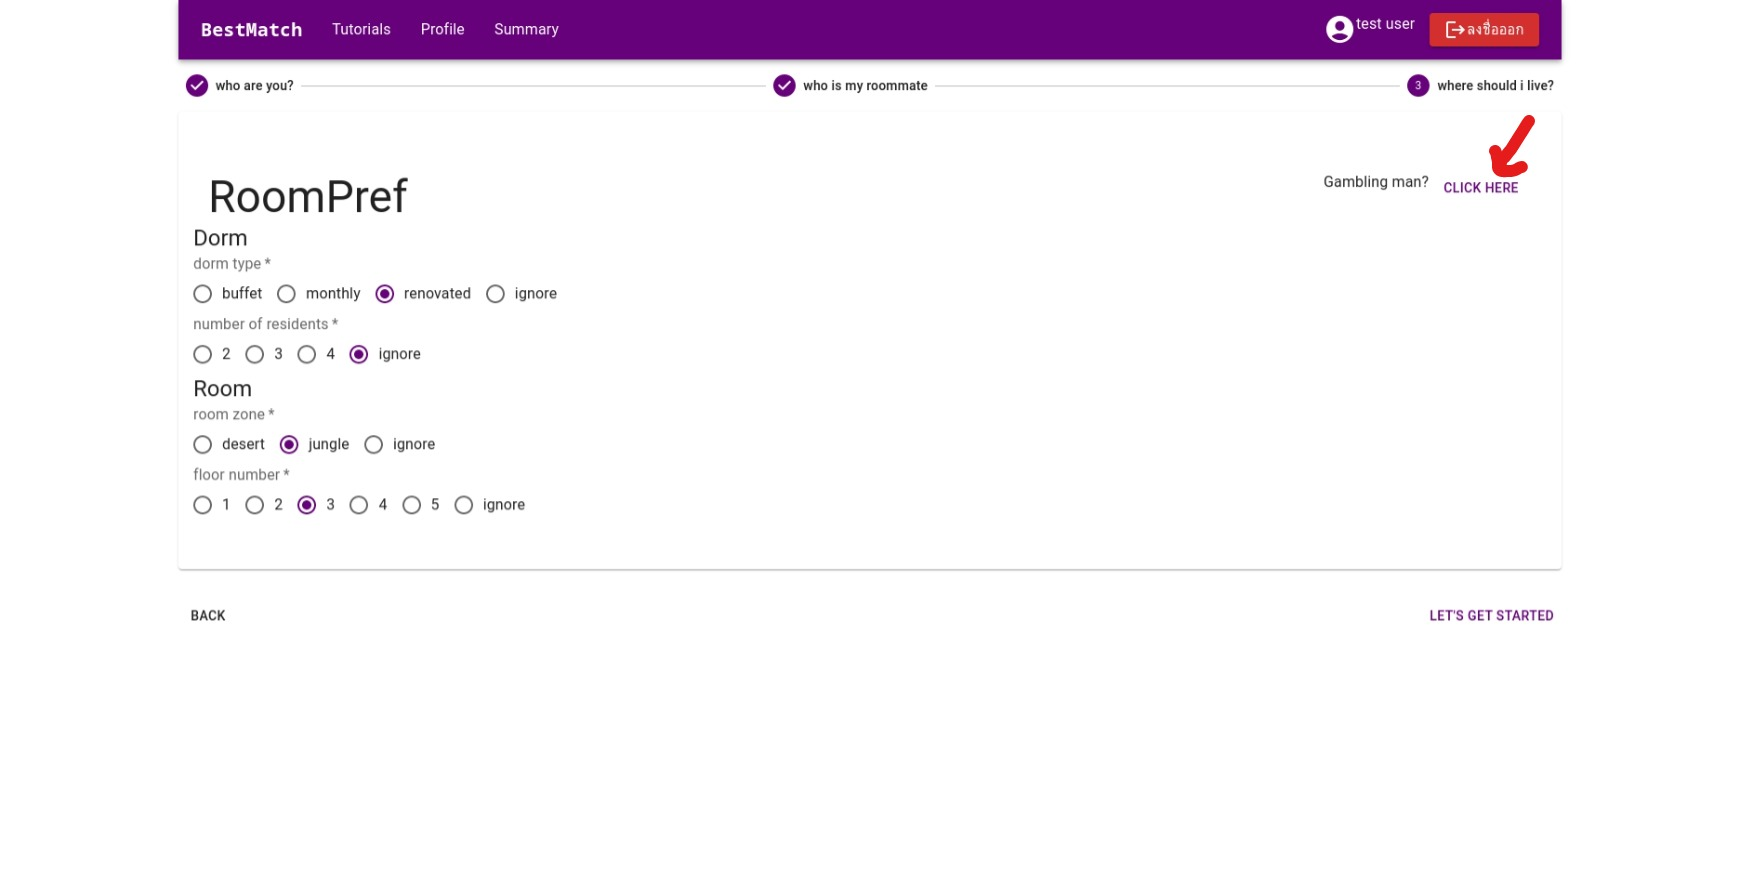
\includegraphics[width=\linewidth]{photo/web/student/dorm-gambler.jpeg}
  \end{center}
  \caption{รูปตัวอย่างแสดงตำแหน่งปุ่ม "CLICK HERE" ของหน้า preference ของหอพัก}
\end{figure}
\newpage
%
% หลังจากนั้นจะเป็นหน้าที่ให้ผู้ใช้เลือกว่าจะเอาโปรไฟล์สมมุติ โปรไฟล์ไหนสำหรับการ finetune
% \begin{figure}[h]
%   \begin{center}
%     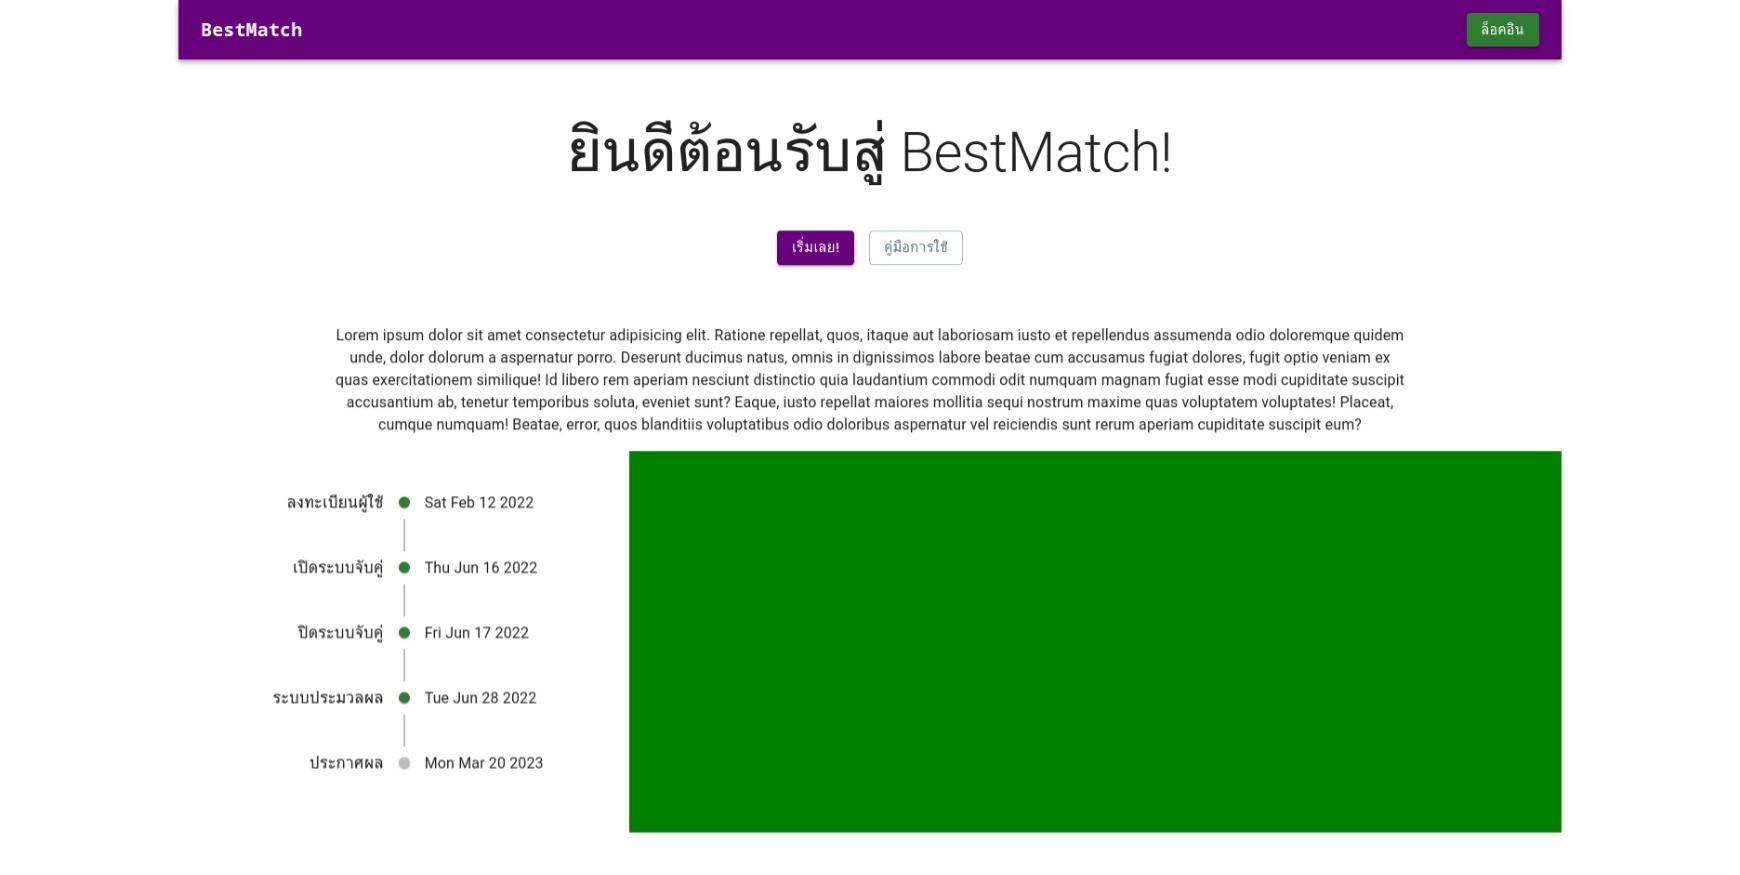
\includegraphics[width=\linewidth]{photo/web/student/home.jpeg}
%   \end{center}
%   \caption{หน้า Home}
% \end{figure} 
% %
% \newline
% หากผู้ใช้พึงพอใจกับการ finetune แล้วสามารถกลับหน้า Home ได้โดยคลิกที่ไอคอน "BESTMATCH"
% \begin{figure}[h]
%   \begin{center}
%     
\includegraphics[width=\linewidth]{photo/web/student/icon-btn.jpeg}
%   \end{center}
%   \caption{รูปตัวอย่างแสดงตำแหน่งปุ่มไอคอน "BESTMATCH"}
% \end{figure}
% \newpage
%
ซึ่งผู้ใช้สามารถตรวจสอบโปรไฟล์ของตนเองได้ที่หน้า Profile
\begin{figure}[h]
  \begin{center}
    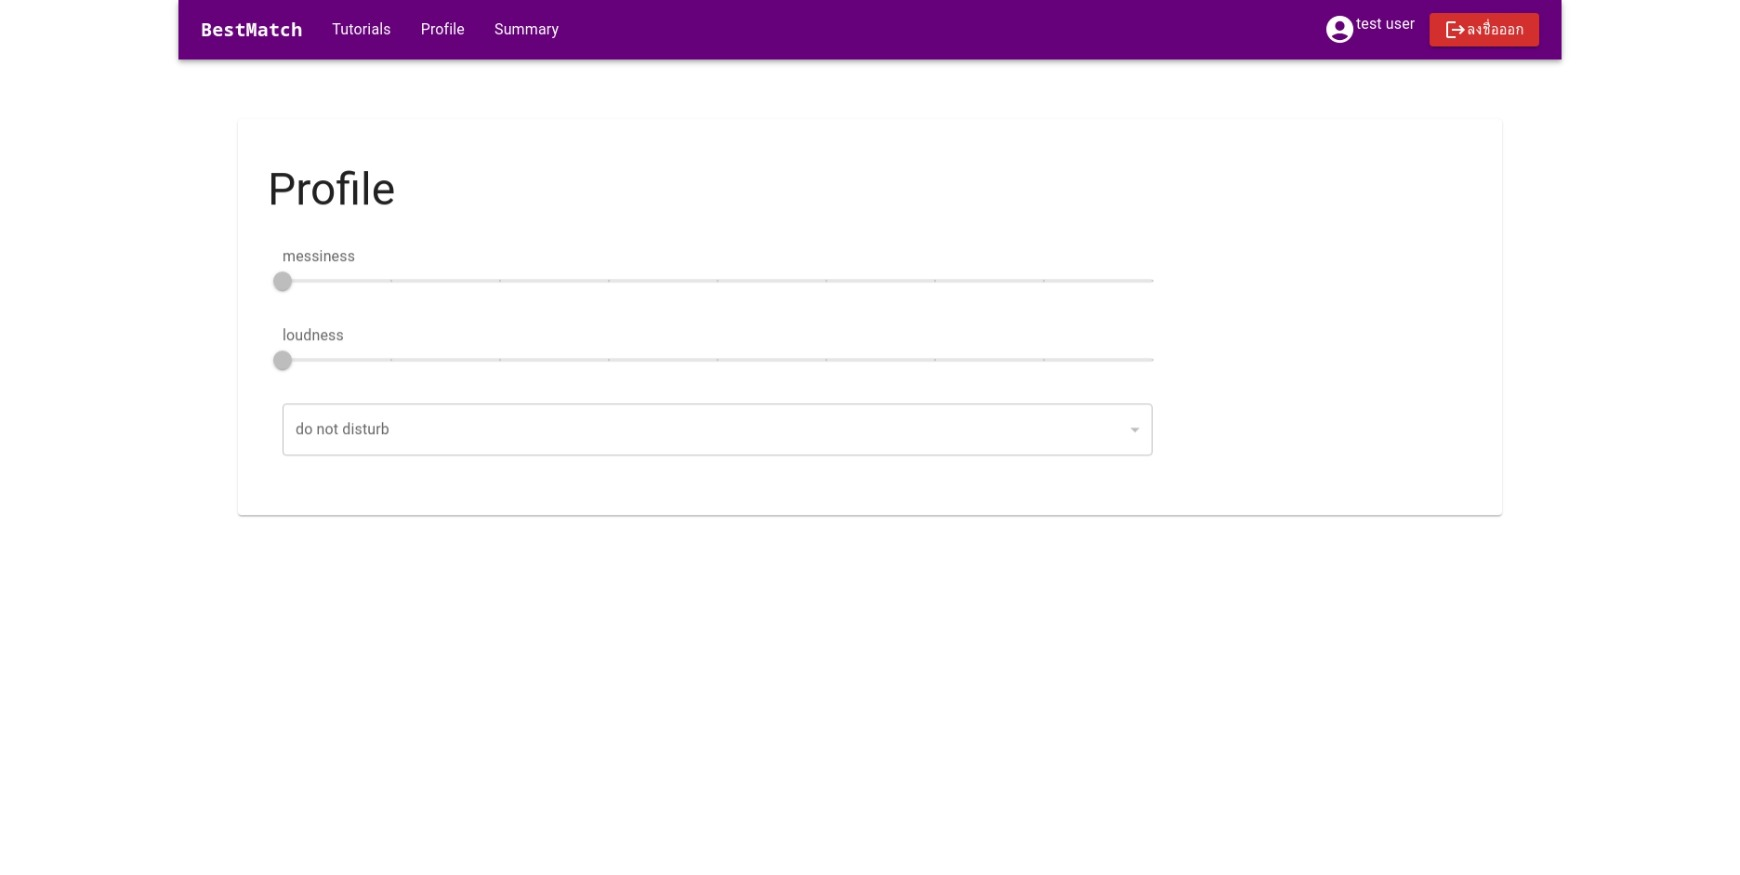
\includegraphics[width=\linewidth]{photo/web/student/profile.jpeg}
  \end{center}
  \caption{หน้า Profile}
\end{figure}
%
\newline
และสามารถตรวจสอบรูมเมทที่คาดว่าจะได้จากการจับคู่ที่หน้า Summary
\begin{figure}[h]
  \begin{center}
    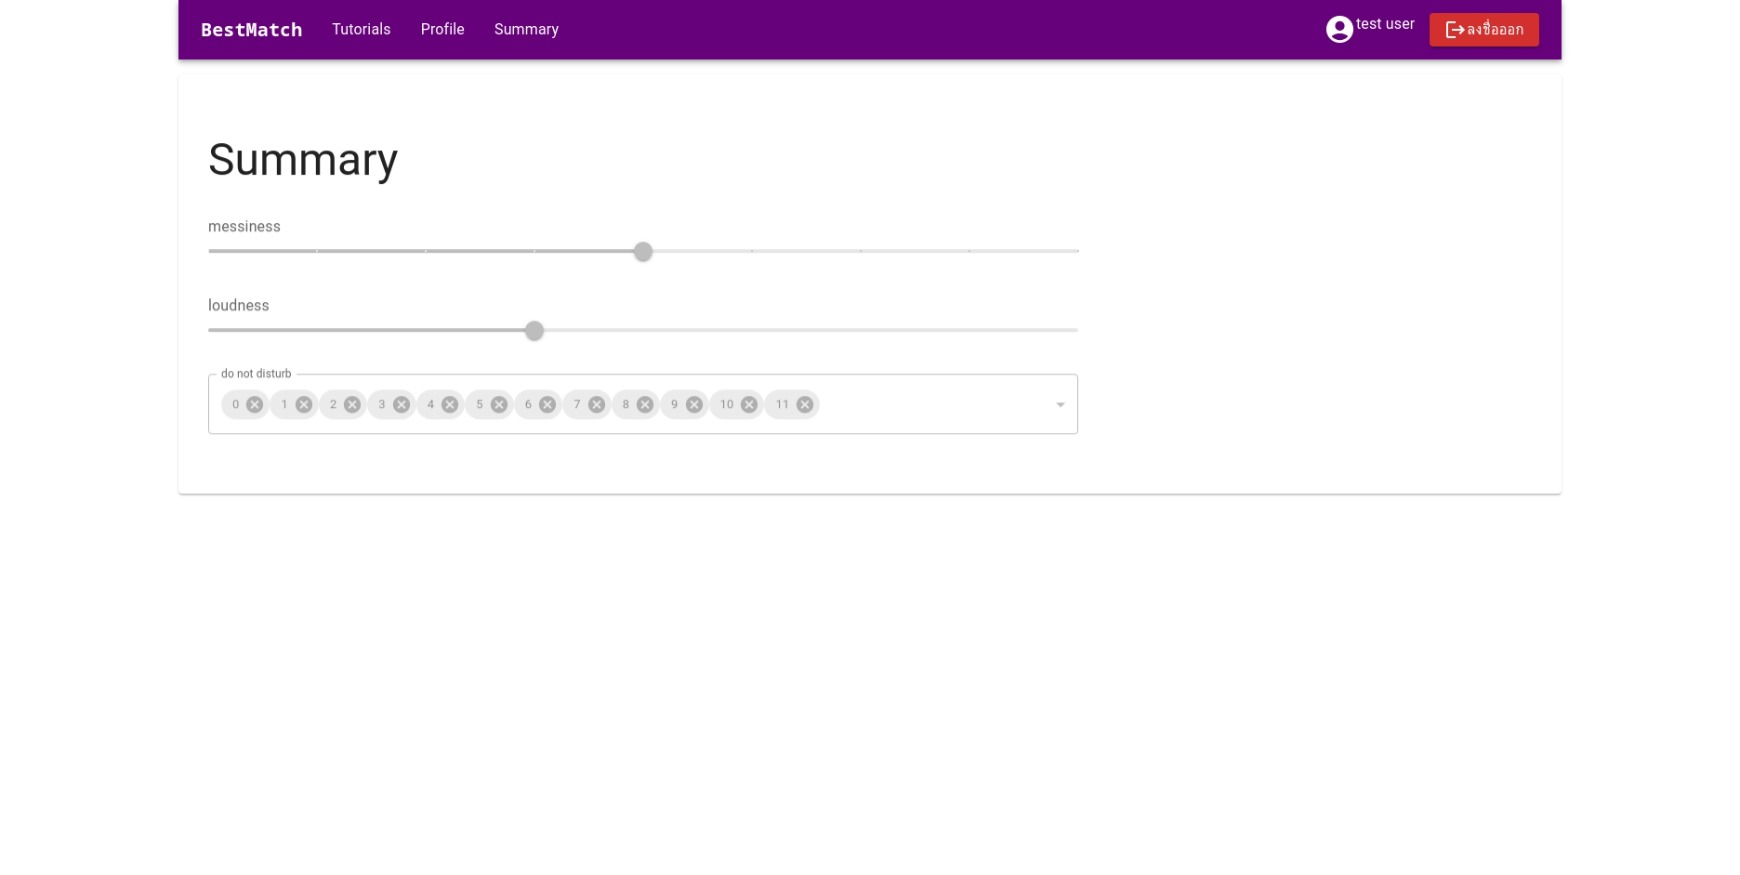
\includegraphics[width=\linewidth]{photo/web/student/summary.jpeg}
  \end{center}
  \caption{หน้า Summary}
\end{figure}

%% Display glossary (optional) -- need glossary option.
\ifglossary\glossarypage\fi

%% Display index (optional) -- need idx option.
\ifindex\indexpage\fi

\begin{biosketch}
\begin{center}
  
\includegraphics[width=1.5in]{photo.old/mugshot.jpg}
\end{center}
Your biosketch goes here. Make sure it sits inside
the \texttt{biosketch} environment.
\end{biosketch}
\fi % \ifproject
\end{document}
